\section{Abstract}\label{sec:paper1_abstract}
Prediction via deterministic continuous-time models will always be subject to model error, for ex ample due to unexplainable phenomena, uncertainties in any data driving the model, or discretisation/resolution issues. 
A standard method for uncertainty quantification in such instances is to introduce noise into the system, and use stochastic simulations to empirically obtain error distributions. 
To supplement this computationally expensive approach, we develop an explicit and computable time-evolving uncertainty distribution for stochastic differential equations with small multiplicative noise. 
For any initial condition, we rigorously establish convergence bounds for all moments of the deviation of the stochastic solution from its linearised counterpart. 
This result extends previous work, that showed the convergence of the Kullback-Leibler divergence. We provide a characterisation of the Gaussian distribution that is the solution to the linearised equation, expressed explicitly in terms of solutions to a reference deterministic model.
This characterisation provides a practical framework for quantifying uncertainty in deterministic differential equation models, with applications including oceanographic and atmospheric modelling, data assimilation and Lagrangian coherent structure extraction

\section{Introduction}\label{sec:paper1_intro}
Many phenomena across geophysical, biological and socio-economic applications can be modelled using a continuous-time dynamical system, i.e., an ordinary differential equation \cite[e.g.]{BrauerCastillo-Chavez_2012_MathematicalModelsPopulation,TelEtAl_2005_ChemicalBiologicalActivity,Wiggins_2005_DynamicalSystemsApproach}. 
Given initial values of a multi-dimensional state variable, such equations can be solved numerically to predict the state at future times.
The governing dynamics may be specified using existing phenomenological models, but in modern applications these are usually supplemented or driven by observed data.  
Standard examples include the modelling of weather using available data \cite{LawEtAl_2015_DataAssimilationMathematical,ReichCotter_2015_ProbabilisticForecastingBayesian}, and predicting concentrations of, for instance, temperature, pollutants or phytoplankton in the ocean using observed current velocity data \cite{AbascalEtAl_2009_ApplicationHFRadar,dOvidioEtAl_2010_FluidDynamicalNiches}.

All methods using this approach have uncertainties in the model specification arising from a variety of sources \cite{FangEtAl_2020_DisentanglingResolutionPrecision}: the model not capturing all phenomena because of the inevitable lack of a complete understanding of all processes involved, errors in measured data, information only available on spatio-temporal grids (resolution error), etc.  
In the absence of any other understanding of these multitudinous issues, a well-established way of tackling such uncertainties in the model is to think of these as stochastic 
\cite{BernerEtAl_2017_StochasticParameterizationNew,Oksendal_2003_StochasticDifferentialEquations}. 
Running many realisations of stochastic perturbations to the deterministic model can generate statistics to improve predictions and estimate their associated uncertainties \cite[e.g.]{BadzaEtAl_2023_HowSensitiveAre,Collins_2007_EnsemblesProbabilitiesNew}.
However, in practice a very large number of simulations is necessary to generate convergent statistics \cite{FepponLermusiaux_2018_DynamicallyOrthogonalNumerical, Leutbecher_2019_EnsembleSizeHow}.
Thus, numerically solving such stochastic systems -- potentially with data-based terms -- is often computationally expensive, and does not necessarily provide conceptual insight into how the model uncertainties affect predictions.

Clearly, possessing a broader theoretical understanding of how stochastic terms impact continuous dynamical systems would be valuable.  
Stochastic differential equations (SDEs) provide a natural framework for introducing uncertainty, as a noise process, into the continuous time evolution of a variable.
Generally, in modelling situations the dynamics are highly nonlinear and one expects the noise to be multiplicative (i.e. vary with both state and time), e.g. in atmospheric \cite{Sura_2003_StochasticAnalysisSouthern, SuraEtAl_2005_MultiplicativeNoiseNonGaussianity} and oceanic \cite{KamenkovichEtAl_2015_PropertiesOriginsAnisotropic} systems and from experimental and observational considerations.
Such SDEs are intractable to solve analytically \cite{Oksendal_2003_StochasticDifferentialEquations} and computationally expensive to simulate accurately \cite{MoraEtAl_2017_StableNumericalScheme}.
Having a data-based model---that is, possessing terms in the equations which are driven by data rather than by explicitly specified functions---renders additional problems in obtaining a theoretical understanding of the prediction error.  

A common intuitive approach to characterising the uncertainty arising from an otherwise analytically intractable nonlinear SDE is via a multivariate Gaussian approximation, which is used across a diversity of literature. 
For instance, one can formally ``linearise'' the SDE in some sense to obtain a Gaussian density, and this approach is used in filtering theory \cite{Jazwinski_2014_StochasticProcessesFiltering}.
Other approaches first assume a Gaussian distribution and obtain formal computations for its mean and covariance \cite{SarkkaSolin_2019_AppliedStochasticDifferential}.
However, both approaches lack rigorous justification and a precise understanding of \emph{how} the Gaussian distribution arises from the nonlinear SDE.
This is particularly the case when the noise is multiplicative, which is a situation that is often ignored but necessary in practice.
Sanz-Alonso and Stuart \cite{Sanz-AlonsoStuart_2017_GaussianApproximationsSmall} partially addressed these issues, by showing that the Kullback-Leibler (KL) divergence between the solutions of autonomous SDEs with additive noise and a linearised equivalent can be bounded by the scale of the noise. In this manuscript, we relax the hypotheses of \cite{Sanz-AlonsoStuart_2017_GaussianApproximationsSmall} to cater for time-dependent coefficients and for multiplicative noise. Furthermore, our result explicitly establishes the convergence rate of all moments of the deviation considered in \cite{Sanz-AlonsoStuart_2017_GaussianApproximationsSmall}, which cannot be inferred from the KL divergence alone.


% In general, however, a rigorous justification (in the sense of a limit, say) of such Gaussian approximations is lacking \cite{Sanz-AlonsoStuart_2017_GaussianApproximationsSmall} when the SDE includes \emph{both} time-dependent coefficients and multiplicative noise.
% A natural theoretical approach in the limit of small noise is to use a linearisation process for the SDE, reducing the otherwise analytically intractable SDE to a solvable linear one. 
% Within the perspective of determining an uncertainty distribution for a prediction, though, such a linearisation has not been rigorously justified \cite{Sanz-AlonsoStuart_2017_GaussianApproximationsSmall}.  
% Other approaches first assume a Gaussian distribution (again, without justification), and obtain formal computations for its mean and covariance \cite{SarkkaSolin_2019_AppliedStochasticDifferential}.
% \sab{Perhaps make a direct quotation here about the fact that this is not justified}

% We remedy these issues in this paper by developing an exact expression for a stochastic process such that solutions to the noisy SDE converge to this process in a precise fashion in the limit of small noise: notably, the expectation of the $ r $th mean of the difference between these converges at a rate of the $ r $th power of the noise parameter for any finite time for all $ r \ge 1 $ (see \Cref{thm:main}). 
In this paper, we remedy this deficiency by proving rigorously that the noise-scaled deviation between the SDE solution and a reference deterministic solution converges towards a multivariate Gaussian distribution, in the limit of small noise.
We consider a general class of SDEs with fully non-autonomous terms and multiplicative noise.
The Gaussian distribution arises as the solution to a formal linearisation of the SDE about a deterministic trajectory (in the absence of noise).
By bounding all raw moments of the difference between the SDE and the linearised solutions by the noise scale (see \Cref{thm:main}), we show that the stochastic deviation converges in distribution to a multivariate Gaussian random variable (see \Cref{thm:gauss_dist}). 
The covariance matrix characterising this Gaussian can be explicitly written in terms of the flow map of the underlying deterministic system and the (potentially spatio-temporally varying) diffusion matrix, and is available even if the deterministic model is only available via data.
The Gaussian distribution is consistent with that seen in other literature \cite{Jazwinski_2014_StochasticProcessesFiltering, Sanz-AlonsoStuart_2017_GaussianApproximationsSmall, SarkkaSolin_2019_AppliedStochasticDifferential}, while we additionally show convergence of \emph{all} the moments of the deviation distribution.
The results hold independently of the initial condition and for all finite times; the uncertainty evolution of any deterministic trajectory with time is therefore encapsulated in our results.

The quantification of prediction uncertainty that we present here was originally motivated by the ``stochastic sensitivity'' approach of Balasuriya \cite{Balasuriya_2020_StochasticSensitivityComputable}.
In the context of two-dimensional, unsteady fluid flow, stochastic sensitivity works with Eulerian velocity data as the underlying deterministic model, and seeks to quantify the uncertainty in an eventual Lagrangian trajectory location.
This methodology was developed as a tool for determining Lagrangian coherent structures (LCS) \cite{BalasuriyaEtAl_2018_GeneralizedLagrangianCoherent,HadjighasemEtAl_2017_CriticalComparisonLagrangian} in fluid flows, in that clusters of trajectories which have small uncertainty may be thought of as more ``coherent'' than others.  
In particular, \cite{Balasuriya_2020_StochasticSensitivityComputable} derived the limiting mean and variance of the noise-scaled deviation, and provided computable expressions in terms of the deterministic flow map and velocity field.
However, this was restricted to two-dimensional systems and did not characterise the limiting distribution itself.

% {For discussion, my opinions: \\
% 1. Perhaps less focus on DA, stochastic parametrisation as the primary motivators for the paper. These are applications down-the-line but not the main target of this paper. \\
% 2a. I think stochastic sensitivity should come up earlier. "\cite{Balasuriya_2020_StochasticSensitivityComputable} derived the mean and covariance of a mathematical construct, albeit in two physical dimensions only. This paper extends the calculation of SS to arbitrary dimensions and additionally proves that SS is Gaussian" is a nice sentence!\\
% 2b. Consider including something on the Fokker-Planck equation (FPE)---and impossibility of exact solution---and then on the alternatives: simulating SDEs many times or approximations. \\
% 3. Point 2 leads nicely into discussing linearisations. I think you have
% \begin{enumerate}[label=(\roman{*}), ref=(\roman{*})]  
%  \item Jazwinski: gives the linearisation but as a Taylor series
%  \item Sanz-Alonso: provides an error bound for the linearisation in terms of the KL divergence, but for additive noise
%  \item Sarkka: \cite[\S5.5]{SarkkaSolin_2019_AppliedStochasticDifferential} gives a general expression for all moments of the sde solution, but one that requires the exact solution to the FPE. \cite[9.1]{SarkkaSolin_2019_AppliedStochasticDifferential} then discusses a \emph{Gaussian assumed density approximation}, that allows calculation of the moments of the sde, but without rigorous justification. 
% \end{enumerate}
% }  


The contributions of this work are:
\begin{itemize}
    \item In \Cref{sec:theory}, we prove rigorously that all moments of the noise-scaled solution to a multidimensional stochastic differential equation with non-autonomous coefficients and multiplicative noise converges towards those of a linearised SDE, in the limit of small noise. 
    % Be clear here. Two sentences - often lacks justification, OR when the justification is there, only additive or autonomous. "Albeit"
    The Gaussian distribution solving the linearised SDE appears in other literature and applications but often lacks justification \cite{Jazwinski_2014_StochasticProcessesFiltering, SarkkaSolin_2019_AppliedStochasticDifferential}. 
    On the other hand, when the linearisation is justified, this is disregarding time-dependence in the coefficients and multiplicative noise \cite{Sanz-AlonsoStuart_2017_GaussianApproximationsSmall}.
    
    \item We present characterisations of the limiting Gaussian distribution in terms of gradients of \emph{either} the velocity field (as an ODE consistent with that arising elsewhere \cite{Jazwinski_2014_StochasticProcessesFiltering, Sanz-AlonsoStuart_2017_GaussianApproximationsSmall, SarkkaSolin_2019_AppliedStochasticDifferential}) or the deterministic flow map. 
    The latter is an alternative characterisation that allows the Gaussian distribution to be computed \emph{entirely from the solution dynamics} of a determinstic model and specification of any multiplicative noise effects known prior.

    \item In \Cref{sec:theory_s2}, we generalise the two-dimensional stochastic sensitivity approach of \cite{Balasuriya_2020_StochasticSensitivityComputable} to arbitrary dimensions.  
    Our expressions enable the computation of stochastic sensitivity in any dimension, as a scalar measure of uncertainty about any solution trajectory of the deterministic model.
    This also extends stochastic sensitivity as a means of Lagrangian coherent structure extraction to fluid flows of arbitrary dimension.

    \item In \Cref{sec:numerics}, we validate the results of \Cref{sec:theory} using stochastic simulations from a 2-dimensional model.
    In particular, we demonstrate that the first four moments of the distance between the realisations and the Gaussian limit follow the predicted bound.
    We also illustrate a key prediction from \Cref{sec:theory_s2}; that the computable covariance matrix of the Gaussian limit captures the time-evolution of uncertainty, even when the noise is multiplicative.
    
\end{itemize}

% In full, we therefore present a framework for ascribing uncertainty distributions to solutions of a deterministic model, characterised \emph{entirely from the solution dynamics} of the model and specification of any multiplicative noise effects known \emph{a priori}.
% The Gaussian distribution is rigorously established as a small noise limit, and serves as both an intrinsic characterisation of the impact of model dynamics on uncertainty, and as an approximate SDE solution.
% By accounting for multiplicative noise, the framework can capture any non-uniform uncertainty known prior.\jm{This feels like the third time the result is discussed in detail. I appreciate the slow build up, but can/should we shorten?}
% Discuss stochastic parameterisation here. Start with "Since this work is fundamental, we do not explicitly consider the parameters. However, the hope is that the work can aide the analysis of parameterisations or provide computationally efficient scheme.

This work is relevant to the well-known ``stochastic parameterisation'' approach in weather and climate modelling, in which stochastic components are introduced to account for unresolved subgrid effects \cite{BernerEtAl_2017_StochasticParameterizationNew,LeutbecherEtAl_2017_StochasticRepresentationsModel,Palmer_2019_StochasticWeatherClimate}.
Since this work is fundamental, in establishing a convergence result for a general class stochastic differential equations, we do not explicitly describe how to construct an appropriate stochastic parameterisation (e.g. specification of the coefficients of the SDE).
Instead, we expect that this result will be useful in the analysis of stochastic parameterisations, and to convert otherwise computationally expensive schemes into an efficient approximations, a goal explicitly identified in \cite{LeutbecherEtAl_2017_StochasticRepresentationsModel}.
We also expect that this work will find application in data assimilation \cite{BudhirajaEtAl_2019_AssimilatingDataModels,Jazwinski_2014_StochasticProcessesFiltering,LawEtAl_2015_DataAssimilationMathematical,ReichCotter_2015_ProbabilisticForecastingBayesian}, as a means of characterising forecast uncertainty.
The original stochastic sensitivity tools have been applied to identify Lagrangian coherent structures (LCSs) in 2-dimensional fluid flow \cite{BadzaEtAl_2023_HowSensitiveAre, Balasuriya_2020_StochasticSensitivityComputable}.
By extending the theory of these tools into arbitrary dimensions, our results can also be used to extract coherent structures in \(n\)-dimensional flows.
These potential applications are discussed in \Cref{sec:discussion}.

% This paper is organised as follows. 
% \Cref{sec:theory} constructs the Gaussian limit and establishes the characterisation in terms of gradients of the flow map. 
% \Cref{sec:theory_s2} extends the definition and computation of stochastic sensitivity in the original work \cite{Balasuriya_2020_StochasticSensitivityComputable} to the \(n\)-dimensional setting, in terms of the covariance matrix characterising the Gaussian limit.
% The theoretical results are demonstrated numerically in \Cref{sec:numerics}, on an idealised meandering jet model for which the velocity field is known.
% \Cref{sec:discussion} details some of the many anticipated applications and theoretical extensions of this work. 

% \sab{Might need to take some of the information below and see whether it can be weaved into the above discussion. }

% \td{END INTRODUCTION HERE}


% For sufficiently small noise, the stochastic solution can be formally written as a power series in the noise scale \cite{Blagoveshchenskii_1962_DiffusionProcessesDepending}.

% Here, we present a Gaussian approximation for the solution to an \(n\)-dimensional It\^o stochastic differential equation at a fixed time, with small multiplicative Gaussian noise.
% A key contribution of this work is a novel characterisation of this Gaussian approximation entirely in terms of the flow map data and the diffusion matrix, without any reference to the velocity field or stochastic differential equation. 
% This provides a framework for ascribing uncertainties to deterministic models \emph{entirely from the solution dynamics}, without explicit reference to 
% By allowing for multiplicative noise, this framework is highly flexible in accounting for noise that may arise from a range of sources and consequently vary spatiotemporally.
% The justification of the approximation is also novel in the sense that it differs from other attempts to justify similar Gaussian approximations, with, for instance, Kullback-Leibler divergence \cite{Sanz-AlonsoStuart_2017_GaussianApproximationsSmall}.
% \td{Mention how both the drift and diffusion depend on time - more general than that presented elsewhere.}
% Rather, the Gaussian approximation is shown to arise as the limiting distribution of the stochastic differential equation solution, in a similar approach to the one-dimensional work of \cite{LiZhang_2016_ModerateDeviationsCentral}\lb{Might not be needed here, but this is the paper that inspired my approach to the proof.}.\sab{This may then be an important reference to have in the introduction -- see if it can be fitted in in an appropriate place.}

%The characterisation of the Gaussian approximation is in terms of spatial flow map gradients, which are quantities commonly used in the field of Lagrangian coherent structures to capture the nonlinear and unsteady dynamics of solutions \cite{BalasuriyaEtAl_2018_GeneralizedLagrangianCoherent, Haller_2015_LagrangianCoherentStructures}.
%This characterisation therefore establishes new connections between aspects of \td{Explain how this opens up new connections between LCS computation and general SDE approximation.}
%In particular, this may enable new practical schemes that generate Gaussian uncertainties directly from observed solution data, without any reference to the driving differential equation, by employing methods for approximating the flow map gradient directly \cite{Leung_2013_BackwardPhaseFlow, RabenEtAl_2013_ComputationFinitetimeLyapunov}.
% For instance, in Lagrangian data assimilation schemes \cite{ApteEtAl_2008_BayesianApproachLagrangian, ApteJones_2013_ImpactNonlinearityLagrangian, StammerEtAl_2016_OceanDataAssimilation, MacleanEtAl_2017_CoherentStructureApproach, BudhirajaEtAl_2019_AssimilatingDataModels}\lb{Check that each of these are relevant} which improve ongoing predictions along trajectories by accounting for both measurement and model error (the latter which we address here).




%%%%%%%%%%%%%%%%%%%%%%%%%%%%%%%%%%%%%%%%%%%%%%%%%%%%%%%%%%%%
% \chapter{Characterising SDE linearisations: the theory}\label{ch:linear_theory}
In general, stochastic differential equations cannot be solved analytically and instead require numerical simulations, which is significantly limited by the computational expense.
An alternative approach is to approximate the SDE by a simplified one, which can be solved analytically.
A linearisation procedure is one such approach when the noise is small, which replaces the coefficients of the SDE with first-order Taylor expansions.
This linearisation scheme is accordingly used across a range of literature and applications \citep{Jazwinski_2014_StochasticProcessesFiltering,SarkkaSolin_2019_AppliedStochasticDifferential,KaszasHaller_2020_UniversalUpperEstimate,ArchambeauEtAl_2007_GaussianProcessApproximations,Sanz-AlonsoStuart_2017_GaussianApproximationsSmall,LawEtAl_2015_DataAssimilationMathematical,ReichCotter_2015_ProbabilisticForecastingBayesian,BudhirajaEtAl_2019_AssimilatingDataModels,LeGlandWang_2002_AsymptoticNormalityPartially}.
Much is already known about the theory of these linearisations: classical results in the context of small-noise series expansions \citep{Blagoveshchenskii_1962_DiffusionProcessesDepending} and large deviations theory \citep{FreidlinWentzell_1998_RandomPerturbationsDynamical} show that the strong error between SDE solution with a fixed initial condition and that of an appropriate linearisation is bounded.
\citet{Sanz-AlonsoStuart_2017_GaussianApproximationsSmall} establish a strong result, bounding the Kullback-Leibler divergence between the solutions of autonomous SDEs with additive stationary noise and a linearised equivalent. Their result considers both an uncertain initial condition, and the evolving error due to the discrepancy between the models.

In this chapter, we build upon these previous small-noise studies \citep{Blagoveshchenskii_1962_DiffusionProcessesDepending,FreidlinWentzell_1998_RandomPerturbationsDynamical,Sanz-AlonsoStuart_2017_GaussianApproximationsSmall} to provide an explicit bound for the error between a general class of stochastic differential equations and corresponding computable linearisations written in terms of a deterministic system.
Our framework accounts for non-autonomous coefficients, multiplicative noise, and uncertain initial conditions in a stochastic differential equation of arbitrary dimension---a more general situation than that considered by \citet{Blagoveshchenskii_1962_DiffusionProcessesDepending} and \citet{FreidlinWentzell_1998_RandomPerturbationsDynamical}.
In \Cref{sec:theory}, we state the bound, written in terms of both the initial and the ongoing uncertainty, and provide an explicit characterisation of the solution to the linearised SDE including computations for the first two moments.
We directly compare our newly-derived bound to that on the KL-divergence by \citet{Sanz-AlonsoStuart_2017_GaussianApproximationsSmall}, and postulate that our bound is tighter.

The second contribution of this chapter is to provide theoretical and computational extension to the original formulation of stochastic sensitivity by \citet{Balasuriya_2020_StochasticSensitivityComputable}, in \Cref{sec:theory_s2}.
We provide a definition of stochastic sensitivity for \(n\)-dimensions, and establish that the value can be computed from a linearised SDE.


Much of the content in this chapter and the following (\Cref{ch:linear_numerics}) has been submitted as a research article to \textit{Communications in Mathematical Sciences} \citep{BlakeEtAl_2023_ConvergenceStochasticDifferential}, and is currently under review.
The preprint is available on arXiv at \href{https://arxiv.org/abs/2309.16334}{arXiv:2309.16334}.
\Cref{sec:ftle_s2_connection}, which discusses the connections between stochastic sensitivity and the finite-time Lyapunov exponent, does not appear in the submitted article, and is instead a new contribution in this thesis.


\section{Convergence of a SDE to a linearisation}\label{sec:theory}
Suppose we are interested in the evolution of a \(\R^n\)-valued state variable \(y_t\) over a finite time interval \([0,T]\).
Our model, accounting for uncertainties arising from a range of sources, for the evolution of this variable is the It\^o stochastic differential equation
\begin{equation}
	\dif y_t^{(\epsilon)} = u\!\left(y_t^{(\epsilon)}, t\right)\dif t + \epsilon \, \sigma\!\left(y_t^{(\epsilon)}, t\right)\dif W_t, \quad y_0^{(\epsilon)} = x
	\label{eqn:sde_y}
\end{equation}
where \(u\colon \R^n \times [0,T] \to \R^n\) is the governing reference vector field.
The canonical \(m\)-dimensional Wiener process \(W_t\)  is a continuous white-noise stochastic process with independent Gaussian increments.
The scale of the ongoing noise is assumed to be small and is parameterised as \(0 < \epsilon \ll 1\).
The noise in \cref{eqn:sde_y} is multiplicative, in that the diffusion matrix \(\sigma\colon \R^n \times [0,T] \to \R^{n\times m}\) can vary with state \( x \), as well as with time \( t \).
We assume that \(\sigma\) is specified \textit{a priori}, or if no such information is known, then \(\sigma \equiv I\), the \(n \times m\) identity matrix, is a default modelling choice.
We consider \cref{eqn:sde_y} subject to the \emph{general} uncertain initial condition \(y_0^{(\epsilon)} = x\), where \(x\) is an \(n\)-dimensional random vector with some given distribution. The two sources of randomness, $ x $ and $ W_t $, are assumed independent from each other.

In the absence of any uncertainty (i.e.\ \(\epsilon = 0\) and the initial condition is a known deterministic quantity), \cref{eqn:sde_y} reduces to the ordinary differential equation
\begin{equation}
	\dod{y_t^{(0)}}{t} = u\!\left(y_t^{(0)}, t\right), \quad y_0^{(0)} = x_0.
	\label{eqn:ode_det}
\end{equation}
where the initial condition \(x_0 \in \R^n\) is fixed.
The formal convergence of the stochastic solution \(y_t^{(\epsilon)}\) (under certain conditions on the initial condition) to the deterministic \(y_{t}^{(0)}\) in the limit as \(\epsilon \to 0\) is well-established using the large deviations principle \citep[e.g]{FreidlinWentzell_1998_RandomPerturbationsDynamical}.
We refer to \cref{eqn:ode_det} as the \emph{reference} deterministic model associated with \cref{eqn:sde_y}.
Solutions to the reference deterministic model are more readily available, e.g.\ in terms of computational efficiency when solving numerically, than those of the stochastic model, but do not account for inevitable uncertainty.

Let the flow map \(F_{0}^{t}\colon \R^n \to \R^n\) be the function which evolves an initial condition from time \(0\) to time \(t\) according to the flow of \cref{eqn:ode_det}, i.e.\ \(F_0^t\!\left(x_0\right) = y_t^{(0)}\).

We assume certain smoothness and boundedness conditions on the various terms outlined, which are stated explicitly in \Cref{hyp:smooth}.
Throughout this article, we use the norm symbol \(\norm{\cdot}\) to denote (i) for a vector, the standard Euclidean vector norm, (ii) for a matrix, the spectral norm induced by the Euclidean norm, and (iii) for a 3rd-order tensor, the spectral norm induced by the matrix norm.
The gradient symbol \(\nabla\) generically refers to derivatives with respect to the state variable.

\renewcommand\thehypo{H}
\begin{hypo}\label{hyp:smooth}
	Let the deterministic functions \(u \colon \R^n\times [0,T] \to \R^n\) and \(\sigma \colon \R^n \times [0,T] \to \R^{n\times m}\), and the random initial condition \(x\) be such that:
	\begin{enumerate}[label=(H.\arabic{*}), ref=H.\arabic{*}]
		\item\label{hyp:fm_exists} For all \(t \in [0,T]\) flow map \(F_0^t \colon \R^n \to \R^n\) is well-defined, and continuously differentiable (with respect to the initial condition) with invertible derivative.

		\item\label{hyp:coef_cont} For each \(t \in [0,T]\), the function \(u(\cdot, t): \R^n \to \R^n\) given by \(u(x,t)\) is twice continuously differentiable on \(\R^n\), and each component of the function \(\sigma(\cdot, t): \R^n \to \R^{n\times m}\) given by \(\sigma(x,t)\) is differentiable on \(\R^n\).

		\item\label{hyp:u_bounds} There exists a constant \(K_{\nabla u} \geq 0\) such that for any \(t \in [0,T]\) and \(x \in \R^n\),
		\begin{equation*}
			\norm{\nabla u(x,t)} \leq K_{\nabla u}.
		\end{equation*}
		Equivalently, for all \(t \in [0,T]\), the function \(u\!\left(\cdot, t\right)\) is Lipschitz continuous with Lipschitz constant \(K_{\nabla u}\).

		\item\label{hyp:coef_meas} For each \(x \in \R^n\), the function \(u(x,\cdot) \colon [0,T] \to \R^n\) and each component of the function \(\sigma(x,\cdot) \colon [0,T] \to \R^{n\times m}\) are Borel-measurable on \([0,T]\).

		\item\label{hyp:linear_growth} There exists a constant \(K_L\) such that for any \(t \in [0,T]\) and \(x \in \R^n\),
		\[
			\norm{u\left(x,t\right)} + \norm{\sigma\left(x,t\right)} \leq K_L\left(1 + \norm{x}\right).
		\]

		\item\label{hyp:sigma_deriv_bound} There exists a constant \(K_{\nabla\sigma} \geq 0\) such that for any \(t \in [0,T]\) and \(x \in \R^n\),
		\begin{equation*}
			\norm{\nabla\sigma(x,t)} \leq K_{\nabla\sigma},
		\end{equation*}
		and we take \(K_{\nabla\sigma} = 0\) if there is no spatial dependence in \(\sigma\).
		Equivalently, for all \(t \in [0,T]\), the function \(\sigma\!\left(x, \cdot\right)\) is Lipschitz continuous with Lipschitz constant \(K_{\nabla\sigma}\).

		\item\label{hyp:init_indep} The initial condition \(x\) is defined on the same probability space as \(W_t\), and is independent of \(W_t\) for all \(t \in [0,T]\).

		\item\label{hyp:nnu_bounds} There exists a constant \(K_{\nabla\nabla u} \geq 0\) such that for any \(t \in [0,T]\) and \(x \in \R^n\),
		\[
			\norm{\nabla \nabla u(x,t)} \leq K_{\nabla\nabla u},
		\]
		and we take \(K_{\nabla\nabla} = 0\) if the second spatial derivatives of \(u\) are all zero.

		\item\label{hyp:sigma_bounds} There exists a constant \(K_\sigma \geq 0\) such that for any \(t \in [0,T]\) and \(x \in \R^n\),
		\begin{equation*}
			\norm{\sigma(x,t)} \leq K_{\sigma}.
		\end{equation*}

	\end{enumerate}
\end{hypo}
The conditions \ref{hyp:coef_cont} to \ref{hyp:init_indep} guarantee that \cref{eqn:sde_y} with the initial condition \(y_0 = x\) has a unique strong solution \citep{KallianpurSundar_2014_StochasticAnalysisDiffusion}.
The bound \(K_{\nabla\nabla u}\) placed on the second derivatives of \(u\) in \ref{hyp:nnu_bounds} quantifies exactly when the deterministic dynamics (that is, \(u\)) of \cref{eqn:sde_y} are linear.
Similarly, the bound \(K_{\nabla\sigma}\) on the spatial derivatives of \(\sigma\) in \ref{hyp:sigma_deriv_bound} allows us to distinguish when the noise in \cref{eqn:sde_y} is multiplicative.

Our aim is to construct and formally justify a computable linearisation of \cref{eqn:sde_y} about a trajectory solving the deterministic system \cref{eqn:ode_det}.
To that end, we take a \emph{fixed} initial condition \(x_0 \in \R^n\) to the reference deterministic model \cref{eqn:ode_det} and consider linearising the SDE \cref{eqn:sde_y} about the corresponding trajectory \(F_0^t\!\left(x_0\right)\).
We consider the following linearisation of \cref{eqn:sde_y}:
\begin{equation}
	\dif l_t^{(\epsilon)} = \left[u\!\left(F_0^t\!\left(x_0\right), t\right) + \nabla u\!\left(F_0^t\!\left(x_0\right), t\right)\left(l_t^{(\epsilon)} - F_0^t\!\left(x_0\right)\right)\right] \! \dif t + \epsilon\sigma\!\left(F_0^t\!\left(x_0\right), t\right) \! \dif W_t, \quad l_0^{(\epsilon)} = x,
	\label{eqn:linear_sde_inform}
\end{equation}
where the initial condition \(x \) is still permitted to be random.
Informally, we can arrive at \cref{eqn:linear_sde_inform} by performing a Taylor expansion of the coefficient \(u\) up to first-order and \(\sigma\) to zeroth-order about the time-varying trajectory \(F_0^t\!\left(x_0\right)\).
Such a linearisation is advantageous over the nonlinear SDE \cref{eqn:sde_y}, since \cref{eqn:linear_sde_inform} can be solved analytically.
We will later (see \Cref{cor:limit_moments}) provide explicit expressions for computing the distribution of the solution \(l_t^{(\epsilon)}\) solely in terms of the solution dynamics of the deterministic system \cref{eqn:ode_det}, the specified diffusion matrix \(\sigma\), and the distribution of \(x\).


In order to quantify the error arising from the choice of reference point \(x_0\), we define
\[
	\delta_r \coloneqq \avg{\norm{x - x_0}^r}^{1/r},
\]
i.e.\ \(\delta_r\) is the \(L_r\) distance between \(x\) and the deterministic point \(x_0\).
We can think of \(\delta_r\) as a scalar measure of the uncertainty in the initial condition, relative to the choice of reference point \(x_0\).
Alternatively, the limit as \(\delta_r\) approaches zero is equivalent to convergence in \(r\)th mean of \(x\) to the fixed point \(x_0\).
We can therefore distinguish two sources of uncertainty in our model; that arising from the initial condition, quantified by \(\delta_r\), and the ongoing uncertainty driven by the Wiener process \(W_t\) as measured by \(\epsilon\).

Our first and primary result, \Cref{thm:main}, provides an explicit bound on the \(r\)th moment of the error between the SDE solution \(y_t^{(\epsilon)}\) and the linearised solution \(l_t^{(\epsilon)}\).


\begin{theorem}[Linearisation error is bounded]\label{thm:main}
	Let \(y_t^{(\epsilon)}\) be the strong solution to the SDE \cref{eqn:sde_y} and \(l_t^{(\epsilon)}\) be the strong solution to the corresponding linearisation \cref{eqn:linear_sde_inform}, both driven by the same Wiener process \(W_t\) and subject to the same random initial condition \(y_0^{(\epsilon)} = l_0^{(\epsilon)} = x\).
	Then, for any \(r \geq 1\) such that \(\delta_{2r} < \infty\) and \(t \in [0,T]\), there exist constants \( D_1\!\left(r,t, K_{\nabla u}, K_{\sigma}\right), \, D_2\!\left(r,t, K_{\nabla u}\right), \, D_3\!\left(r,t, K_{\nabla u}\right) \in [0, \infty) \) independent of \(x\) and \(x_0\) such that for all \(\epsilon > 0\),
	\begin{equation}
		\avg{\norm{y_t^{(\epsilon)} - l_t^{(\epsilon)}}^r} \leq \begin{multlined}[t]
			\left(K_{\nabla\nabla u}^r + K_{\nabla\sigma}^r\right) D_1\!\left(r,t, K_{\nabla u}, K_\sigma\right)\, \epsilon^{2r} \\
			+ K_{\nabla\nabla u}^r D_2\!\left(r,t, K_{\nabla u}\right)\delta_{2r}^{2r}
			+ K_{\nabla\sigma}^r D_3\!\left(r,t, K_{\nabla u}\right)\delta_r^r \epsilon^r.
		\end{multlined}
		\label{eqn:main_ineq}
	\end{equation}
\end{theorem}

\begin{proof}
	See \Cref{app:main_thm_proof}.
	Our proof employs the Burkholder-Davis-Gundy inequality, Gr\"onwall's inequality, and Taylor's theorem to explicitly construct the bounding coefficients in terms of the conditions on the SDE coefficients set out in \Cref{hyp:smooth}.
	The bounding coefficients \(D_1\), \(D_2\), and \(D_3\) are given explicitly in \cref{eqn:bound_defns}.
\end{proof}


In \cref{eqn:main_ineq}, we have an explicit scaling of the error in terms of \(\epsilon\) and \(\delta_r\).
The three terms can be informally considered as: a contribution purely from the ongoing linearisation error, a contribution purely from the initial uncertainty, and a term resulting from the interaction between the initial and ongoing uncertainties.
By explicitly identifying the dependence of the bound on \(K_{\nabla\nabla u}\) and \(K_{\nabla \sigma}\), we note three special cases that are summarised by \Crefrange{rem:bound_linear}{rem:bound_exact}.

\begin{remark}[Linear drift]\label{rem:bound_linear}
	When the deterministic dynamics are linear, we set \(K_{\nabla\nabla u} = 0\) and \cref{eqn:main_ineq} becomes
	\[
		\avg{\norm{y_t^{(\epsilon)} - l_t^{(\epsilon)}}^r} \leq   K_{\nabla\sigma}^r D_1\!\left(r, t, K_{\nabla u}, K_\sigma\right)\, \epsilon^{2r} + K_{\nabla\sigma}^r D_3\!\left(r,t, K_{\nabla u}\right)\delta_r^r \epsilon^r.
	\]
	The linearisation of the drift term \(u\) is exact, so the error is purely due to the spatial dependency of the diffusion term \(\sigma\).
\end{remark}

\begin{remark}[Additive noise]\label{rem:bound_additive}
	When the noise in \cref{eqn:sde_y} is additive, we set \(K_{\nabla\sigma} = 0\) and \cref{eqn:main_ineq} becomes
	\[
		\avg{\norm{y_t^{(\epsilon)} - l_t^{(\epsilon)}}^r} \leq   K_{\nabla\nabla u}^r D_1\!\left(r,t, K_{\nabla u}, K_\sigma\right)\, \epsilon^{2r} + K_{\nabla\nabla u}^r D_2\!\left(r,t, K_{\nabla u}\right)\delta_{2r}^{2r}.
	\]
	The error is then purely due to the linearisation of the drift term \(u\), and as expected is of second order in both the initial condition uncertainty \(\delta_{2r}\) and the ongoing uncertainty \(\epsilon\).
\end{remark}

\begin{remark}[Exact linearisation]\label{rem:bound_exact}
	When the deterministic dynamics are linear and the noise in \cref{eqn:sde_y} is additive (non-multiplicative), the linearisation \cref{eqn:linear_sde_inform} should be exact.
	Accordingly, we set \(K_{\nabla\nabla u} = K_{\nabla\sigma} = 0\) and \cref{eqn:main_ineq} becomes
	\[
		\avg{\norm{y_t^{(\epsilon)} - l_t^{(\epsilon)}}^r} = 0.
	\]
	In turn, this implies that \(y_t^{(\epsilon)} = l_t^{(\epsilon)}\) almost surely, for any choice of reference point \(x_0\).
\end{remark}


We postpone a discussion of an additional special case---where the initial condition is fixed or
Gaussian---to a later section.  For the general situation,
we next explicitly establish the solution to the linearisation \cref{eqn:linear_sde_inform}, in terms of the initial condition and the deterministic evolution of \cref{eqn:ode_det}.

\begin{theorem}[Solution of the linearised SDE]\label{thm:limit_sol}
	The strong solution to the linearised SDE \cref{eqn:linear_sde_inform} is
	\begin{equation}
		l_t^{(\epsilon)} = \nabla F_0^t\!\left(x_0\right)\left(x - x_0\right) + F_0^t\!\left(x_0\right) + \epsilon\nabla F_0^t\!\left(x_0\right)\int_0^t{L\!\left(x_0, \tau\right)\dif W_\tau}.
		\label{eqn:linear_sol}
	\end{equation}
	where the term involving the uncertain initial condition \(x\) and the It\^o integral are independent, and
	\begin{equation}
		L\!\left(x_0, \tau\right) \coloneqq \left[\nabla F_0^\tau(x_0)\right]^{-1}\sigma\left(F_0^\tau(x_0), \tau\right).
		\label{eqn:sigma_L_def}
	\end{equation}

\end{theorem}
\begin{proof}
	See \Cref{app:limit_sol_proof}.
\end{proof}

The representation of the linearised solution as an independent sum in \cref{eqn:linear_sol} can be seen as a decomposition into contributions from the initial uncertainty (the transformation of initial condition \(x\)), a deterministic prediction (the flow map \(F_0^t\!\left(x_0\right)\)) and the ongoing uncertainty in \(u\) (the remaining It\^o integral term).

We can further show that the It\^o integral term follows a Gaussian random variable, which ensures that the independent sum in \cref{eqn:linear_sol} is a convenient expression for both theoretical analysis and numerical computation.
We also provide explicit expressions for the mean and covariance matrix of the linearised solution, written in terms of the deterministic dynamics and \(\sigma\).
\begin{corollary}[Distribution of the linearised solution]\label{cor:limit_moments}
	The It\^o integral term in \cref{eqn:linear_sol} follows a Gaussian distribution independent of \(x\), namely
	\[
		\int_0^t{L\!\left(x_0,\tau\right)\dif W_\tau} \isGauss{0, \int_0^t{L\!\left(x_0, \tau\right)L\!\left(x_0, \tau\right)^{\T}\dif\tau}}.
	\]
	The mean of the linearised solution is
	\begin{equation}
		\avg{l_t^{(\epsilon)}} = F_0^t\!\left(x_0\right) + \nabla F_0^t\!\left(x_0\right) \avg{x - x_0}.
		\label{eqn:mean_expl_eqn}
	\end{equation}
	The \(n\times n\) covariance matrix of the linearised solution is given explicitly by
	\begin{equation}
		\var{l_t^{(\epsilon)}} = \nabla F_0^t\!\left(x_0\right)\left(\var{x} + \epsilon^2 \int_0^t{L\!\left(x_0,\tau\right)L\!\left(x_0,\tau\right)^{\T}\dif\tau}\right)\left[\nabla F_0^t\!\left(x_0\right)\right]^{\T}
		\label{eqn:pi_expl_eqn}
	\end{equation}
	where \(L\!\left(x_0, \tau\right)\) is as defined in \cref{eqn:sigma_L_def} and the integral is taken in the elementwise sense.
\end{corollary}
\begin{proof}
	See \Cref{app:limit_moments_proof}.
	The expressions follow from the representation of the linearised solution as an independent sum in \cref{eqn:linear_sol}.
\end{proof}

In \Cref{thm:limit_sol}, we have provided expressions for the distribution of the solution \(l_t^{(\epsilon)}\) to the linearised SDE \cref{eqn:linear_sde_inform} written solely in terms of the behaviour of the deterministic system \cref{eqn:ode_det}, the specified diffusion matrix \(\sigma\), and the distribution of the initial condition \(x\).
This describes a method for approximating the solution to the nonlinear SDE \cref{eqn:sde_y}, or for characterising the impact of uncertainty in a dynamical system \cref{eqn:ode_det}, that circumvents the need for expensive stochastic simulation.

Thus far, we have stated our results in terms of a general initial condition \(x\), and provided expressions for the linearised solution in terms of this otherwise arbitrary distribution.
However, we later consider two special cases for the initial condition \(x\), a fixed (deterministic) initial condition in \Cref{sec:theory_fixed}, and a Gaussian initial condition in \Cref{sec:theory_gauss}.
In both these cases, the linearised solution also follows a Gaussian distribution which is characterised entirely by the mean and covariance described in \Cref{cor:limit_moments}, allowing for easy computation.
We also relate these results directly to other literature \citep{Jazwinski_2014_StochasticProcessesFiltering,FreidlinWentzell_1998_RandomPerturbationsDynamical,Blagoveshchenskii_1962_DiffusionProcessesDepending,Balasuriya_2020_StochasticSensitivityComputable,Sanz-AlonsoStuart_2017_GaussianApproximationsSmall,SarkkaSolin_2019_AppliedStochasticDifferential} which uses linearisation procedures and Gaussian process approximations for nonlinear SDEs in these situations.

Next, we establish the ordinary differential equation satisfied by the covariance matrix, which is an expression consistent with linearisations schemes described elsewhere \citep{ArchambeauEtAl_2007_GaussianProcessApproximations,SarkkaSolin_2019_AppliedStochasticDifferential,Jazwinski_2014_StochasticProcessesFiltering,Sanz-AlonsoStuart_2017_GaussianApproximationsSmall}.
This ODE enables rapid computation of the mean and covariance of the linearised solutions by solving a system of ODEs, i.e.\ \cref{eqn:ode_det} and \cref{eqn:pi_ode}.

\begin{remark}\label{rem:cov_ode}
	The \(n\times n\) covariance matrix \(\var{l_t^{(\epsilon)}}\) of the linearised solution is the symmetric positive-semidefinite \(n \times n\) matrix solution to the ordinary differential equation
	\begin{equation}
		\dod{\Pi(t)}{t} = \begin{multlined}[t]
			\nabla u\!\left(F_0^t\!\left(x_0\right), t\right) \Pi(t) + \Pi(t)\left[\nabla u\!\left(F_0^t\!\left(x_0\right), t\right)\right]^{\!\T}\! + \epsilon^2\sigma\!\left(F_0^t\!\left(x_0\right), t\right)\sigma\!\left(F_0^t\!\left(x_0\right), t\right)^{\T}\!,
		\end{multlined}
		\label{eqn:pi_ode}
	\end{equation}
	subject to the initial condition \(\Pi(0) = \var{x}\).
	We show that the variance satisfies \cref{eqn:pi_ode} in \Cref{app:limit_moments_proof}.
\end{remark}





%%%%%%%%%%%%%%%%%%%%%%%%%%%%%%%%%%%%%%%%%%%%%%%%%%%%
\subsection{Comparison to existing results}
\label{sec:comparison}
In this section we connect our work to the cognate bound derived by \citet{Sanz-AlonsoStuart_2017_GaussianApproximationsSmall}.
That paper considers the following SDE:
\begin{equation}\label{eqn:SAS_sde}
	\dif y_t^{(\epsilon)} = u\!\left(y_t^{(\epsilon)}\right)\dif t + \epsilon \, \tilde{\sigma}\dif W_t,
\end{equation}
where the diffusion coefficient \(\tilde{\sigma}\) is a constant matrix, which is a special case of \cref{eqn:sde_y}.
In this section, we apply our results to \cref{eqn:SAS_sde} to enable both bounds to be compared.
Note that \(\epsilon\) in our article is written as \(\sqrt{\epsilon}\) in \citet{Sanz-AlonsoStuart_2017_GaussianApproximationsSmall}; we will translate results from \citet{Sanz-AlonsoStuart_2017_GaussianApproximationsSmall} to use our notation, so that all results in this article are directly comparable.
In the following, \(c\) denotes an arbitrary finite and non-negative constant that can vary between inequalities.

Theorem 2.2 of \citet{Sanz-AlonsoStuart_2017_GaussianApproximationsSmall}, summarised, is as follows.
Let \(\xi_t^{(\epsilon)}\) be the probability measure associated with \(y_t^{(\epsilon)}\) (as defined in \cref{eqn:SAS_sde}), and let \(\nu_t^{(\epsilon)}\) be the probability measure associated with the corresponding linearisation \(l_t^{(\epsilon)}\) (as defined in \cref{sec:theory}).
Then there exists a constant \(c\) such that the Kullback--Leibler (KL) divergence \(D_{\mathrm{KL}}\) between \(\xi_t^{(\epsilon)}\) and \(\nu_t^{(\epsilon)}\) is bounded;
\begin{equation}
	\label{eqn:SAS}
	D_{\mathrm{KL}}\!\left(\xi_t^{(\epsilon)} \,\middle|\middle|\, \nu_t^{(\epsilon)}\right) \le D_{\mathrm{KL}}\!\left(\xi_0^{(\epsilon)} \,\middle|\middle|\, \nu_0^{(\epsilon)}\right) + c \, \epsilon^2\;.
\end{equation}
To focus on the scaling with \(\epsilon\), assume a fixed initial condition with \(D_{\mathrm{KL}}\!\left(\xi_0^{(\epsilon)} \,\middle|\middle|\, \nu_0^{(\epsilon)}\right) = 0\) (and \(\delta_r = 0\) in our bound \cref{eqn:main_ineq}). Then, employing the Hellinger distance \(D_{\mathrm{H}}\), \cref{eqn:SAS} implies
\begin{align}
	\label{eqn:convert}
	\norm{\avg{ y_t^{(\epsilon)} - l_t^{(\epsilon)}} } \le c D_{\mathrm{H}}\!\left(\xi_t^{(\epsilon)} ,\, \nu_t^{(\epsilon)}\right) \le c \sqrt{D_{\mathrm{KL}}\!\left(\xi_t^{(\epsilon)} \,\middle|\middle|\, \nu_t^{(\epsilon)}\right)} \le c \, \epsilon \;,
\end{align}
while our result \cref{eqn:main_ineq} and Jensen's inequality imply
\[
	\norm{\avg{ y_t^{(\epsilon)} - l_t^{(\epsilon)}} } \le \avg{\norm{y_t^{(\epsilon)} - l_t^{(\epsilon)}}} \leq c \, \epsilon^2\;.
\]
Thus, our bound on the moments is quadratic in \( \epsilon \) rather than linear.
If our conversion in \cref{eqn:convert} was optimal, then our approach in this article
provides a sharper bound on \(\norm{\avg{y_t^{(\epsilon)} - l_t^{(\epsilon)}}}\) that the
results of  \citet{Sanz-AlonsoStuart_2017_GaussianApproximationsSmall} imply, and do so for a
more general $ \sigma $.
The results in  \citet{Sanz-AlonsoStuart_2017_GaussianApproximationsSmall} on the KL divergence would be more natural in information-theoretic contexts, and our hope is that our explicit bound on the moments would be similarly preferred in other contexts.




\subsection{Gaussian initial condition}\label{sec:theory_gauss}
We now briefly consider the case when the initial condition follows a Gaussian distribution, i.e.\ \(x \isGauss{\mu_0, \Sigma_0}\), where \(\mu_0 \in \R^n\) and \(\Sigma_0 \in \R^{n \times n}\) are fixed and specified.
The linearisation then follows a Gaussian distribution itself, which is entirely characterised by the mean and covariance matrix described in \Cref{cor:limit_moments}.
Alternatively, these moments can be conveniently computed by simultaneously solving \cref{eqn:ode_det} for the state variable and \cref{eqn:pi_ode} for the linearised covariance.

A natural choice of reference point \(x_0\) is the mean of the initial Gaussian density, i.e.\ \(x_0 = \mu_0\).
The \(L_r\) distance between \(x\) and the mean \(\mu_0\) can be bounded by the trace of \(\Sigma_0\); for example, one such bound is
\begin{equation}\label{eqn:gauss_dist_bound}
	\delta_r^{r} \leq n^{3r/2 - 1} M_r \mathrm{tr}\left(\Sigma_0\right)^{r/2}, \quad M_r \coloneqq \frac{2^{r/2}\Gamma\!\left(\frac{r + 1}{2}\right)}{\sqrt{\pi}},
\end{equation}
where \(\Gamma\) denotes the Gamma function, with equality when \(n = 1\).
The initial covariance \(\Sigma_0\) directly measures the uncertainty in the initial condition, and we see through \cref{eqn:gauss_dist_bound} that as the components of \(\Sigma_0\) approach zero, the contribution of the initial uncertainty to the linearisation error in \cref{eqn:main_ineq} approaches zero also.
The linearised solution is then
\[
	l_t^{(\epsilon)} \isGauss{F_0^t\!\left(x_0\right), \, \nabla F_0^t\!\left(x_0\right) \Sigma_0\left[\nabla F_0^t\!\left(x_0\right)\right]^{\T} + \varepsilon^2 \Sigma_0^t\!\left(x_0\right)},
\]
where \(\Sigma_0^t\!\left(x_0\right)\) is given explicitly by
\begin{equation}\label{eqn:sigma_def}
	\Sigma_0^t\!\left(x_0\right) = \nabla F_0^t\!\left(x_0\right)\left(\int_0^t{L\!\left(x_0, \tau\right)L\!\left(x_0, \tau\right)^{\T} \dif\tau}\right)\left[\nabla F_0^t\!\left(x_0\right)\right]^{\T},
\end{equation}
and is the solution to the matrix differential equation \cref{eqn:pi_ode} in \Cref{rem:cov_ode}, subject to \(\Sigma_0^0\!\left(x_0\right) = O\), the \(n \times n\) zero matrix.
The covariance matrix \(\Sigma_0^t\!\left(x_0\right)\) characterises the contribution of the ongoing uncertainty in the stochastic system.
The full covariance matrix \(\var{l_t^{(\epsilon)}}\) is also the solution to \cref{eqn:pi_ode} subject to the initial condition \(\Pi(0) = \var{x}\).
By jointly solving \cref{eqn:ode_det} for the deterministic trajectory (the mean of \(l_t^{(\epsilon)}\)) and \cref{eqn:pi_ode} for the covariance matrix, one can easily compute the linearised solution, describing exactly the assumed Gaussian approximation presented in \citet{SarkkaSolin_2019_AppliedStochasticDifferential}, and the dynamics linearisation used in the extended Kalman filter \citep{Jazwinski_2014_StochasticProcessesFiltering}.


%%%%%%%%%%%%%%%%%%%%%%%%%%%%%%%%%%%%%%%%%%%%%%%%%%%%
\subsection{Fixed initial condition}\label{sec:theory_fixed}
Consider when the initial condition \(x\) is itself a fixed and known deterministic value, in which case we take \(x = x_0\) and \(\delta_r = 0\) for all \(r\).
In this situation, the bound \cref{eqn:main_ineq} on the linearisation error reduces to
\begin{equation}
	\avg{\norm{y_t^{(\epsilon)} - l_t^{(\epsilon)}}^r} \leq \left(K_{\nabla\nabla u}^r + K_{\nabla\sigma}^r\right)D_1\!\left(r,t, K_{\nabla u}, K_\sigma\right)\epsilon^{2r}.
	\label{eqn:main_ineq_fixed}
\end{equation}
We can consider the linearisation as equivalently arising from a first-order power series expansion of \(y_t^{(\epsilon)}\) in the noise-scale parameter \(\epsilon\), i.e.
\[
	y_t^{(\epsilon)} = F_0^t\!\left(x_0\right) + \epsilon z_t^{(\epsilon)} + R_2\left(x,t,\epsilon\right).
\]
where \(z_\epsilon \coloneqq \left(l_{t}^{(\epsilon)} - F_0^t\!\left(x_0\right)\right) / \epsilon\) is the first order term and \(R_2\) is a random quantity capturing the remaining deviation between \(y_t^{(\epsilon)}\) and the linearisation.
By rearranging and taking \(r = 1\) in \cref{eqn:main_ineq_fixed}, we therefore have the explicit Taylor-like bound
\[
	\frac{\avg{\norm{R_2\left(x,t,\epsilon\right)}}}{\epsilon^2} \leq \left(K_{\nabla \nabla u} + K_{\nabla\sigma}\right)D_1\!\left(1,t, K_{\nabla u}, K_\sigma\right),
\]
This result is consistent with the formulation of the linearisation error bounds by \citet{Blagoveshchenskii_1962_DiffusionProcessesDepending} and \citet{FreidlinWentzell_1998_RandomPerturbationsDynamical}, for instance.
Moreover, the distribution of the linearisation solution \cref{eqn:linear_sol} is Gaussian, which through \Cref{cor:limit_moments} we can again explicitly characterise in terms of the deterministic system, namely
\begin{equation}
	l_t^{(\epsilon)} \isGauss{F_0^t\!\left(x_0\right), \epsilon^2 \Sigma_0^t\!\left(x_0\right)},
	\label{eqn:linear_gauss_sol}
\end{equation}
where \(\Sigma_0^t\!\left(x_0\right)\) is defined in \cref{eqn:sigma_def}.
The distribution can be computed \emph{entirely} from the solution behaviour of the deterministic equation \cref{eqn:ode_det} and prior specification of \(\sigma\).
In \Cref{sec:theory_s2}, we demonstrate an application of these results to extend stochastic sensitivity \citep{Balasuriya_2020_StochasticSensitivityComputable} to arbitrary dimension.


%%%%%%%%%%%%%%%%%%%%%%%%%%%%%%%%%%%%%%%%%%%%%%%%%%%%
\section{Extending stochastic sensitivity}\label{sec:theory_s2}
The results of \Cref{sec:theory_fixed} for a fixed initial condition provide a direct extension of the stochastic sensitivity tools first introduced by \citet{Balasuriya_2020_StochasticSensitivityComputable} for the fluid flow context.
Here, the deterministic model \cref{eqn:ode_det} is seen as a ``best-available'' model for the evolution of Lagrangian trajectories, and the driving vector field \(u\) is the Eulerian velocity of the fluid.
Stochastic sensitivity ascribes a scalar value to each deterministic trajectory by computing a maximum variance of projected deviation \citep{Balasuriya_2020_StochasticSensitivityComputable}.
The aim is to provide a \emph{single} computable number for each deterministic trajectory quantifying the impact of uncertainty in the velocity, independent of the scale (\(\epsilon\)) of the noise.
The natural restating of this original definition of stochastic sensitivity \citep{Balasuriya_2020_StochasticSensitivityComputable} in the $ n $-dimensional setting is as follows:

\begin{figure}
	\centering
	\begin{tikzpicture}[scale=2]
		\pgfmathsetseed{1}

		% Actual path
		\draw (1,1) .. controls (2.5,-0.5) and (4,1.4) .. (5, 0.5);

		% Stochastic path -- just place a random walk between specified points
		\draw[color=ForestGreen, decorate, decoration={random steps, segment length = 1pt, amplitude=2pt}] (1,1) .. controls (2.5, -0.2) and (3.7,2.7) .. (6.4, 2.1);

		% S2 quantities
		\path[-{Latex[length=3mm, width=1.5mm]},blue] (5,0.5) edge node[left, xshift=-5pt] {\(y_t^{(\epsilon)} - F_0^t\!\left(x_0\right)\)} (6.4, 2.1);
		% Calculation here: fix theta, the angle of the projection. Length of the vector between det point and end of projection is l*sin(n), where l is the length of the vector between the det and stoch points, and n = pi/2 - phi + theta, where phi is the angle of the vector between the det and stoch points.
		\def\vecl{sqrt(1.4^2 + 1.6^2)};
		\def\projtheta{pi/7};
		\def\projphi{atan(1.6 / 1.4) * pi / 180}
		\path[red] (5,0.5) edge ({5 +\vecl*cos((\projphi - \projtheta) r) * cos(\projtheta r)}, {0.5 + \vecl* cos((\projphi - \projtheta) r) * sin(\projtheta r)});

		\path[dashed, gray] (6.4, 2.1) edge ({5 + \vecl * cos((\projphi - \projtheta) r) * cos(\projtheta r)}, {0.5 + \vecl * cos((\projphi - \projtheta) r) * sin(\projtheta r)});

		% Reference angle
		% \path[dashed,gray] (5,0.5) edge (7,0.5);
		% \draw[gray] (5.5,0.5) arc (0:{\projtheta * 180 / pi}:0.5) node[midway, xshift=5pt, yshift=2pt] {\(\theta\)};

		% Instead, we get a vector p
		\path[-{Latex[length=3mm, width=1.5mm]}, gray] (5,0.5) edge node[right, xshift=5pt, yshift=-2pt] {\(p\)} ({5 + cos(\projtheta r)}, {0.5 + sin(\projtheta r)});


		% Points
		\filldraw [black] (1,1) circle (1pt) node[anchor=east] {\(x_0\)};
		\filldraw [black] (5,0.5) circle (1pt) node [anchor=north] {\(F_0^t\!\left(x_0\right)\)};
		\filldraw [color=ForestGreen] (6.4, 2.1) circle (1pt) node [anchor=south] {\(y_t^{(\epsilon)}\)};

	\end{tikzpicture}
	\caption{The entities used in \Cref{def:ss_Rn} of stochastic sensitivity in arbitrary dimensions, which should be compared to \Cref{fig:s2_diag}.
	}
	\label{fig:s2_diag_Rn}
\end{figure}

\begin{definition}[Stochastic sensitivity in \(\R^n\)]\label{def:ss_Rn}
	The \emph{stochastic sensitivity} is a scalar field \(S^2: \R^n \times [0,T] \to \left[0, \infty\right)\) given by
	\begin{equation*}
		S^2\!\left(x_0,t\right) \coloneqq \lim_{\epsilon\downarrow 0}\sup\set{\var{\frac{1}{\epsilon}p^{\T}\left(y_t^{(\epsilon)} - F_0^t\!\left(x_0\right)\right)} \,: \, p \in \R^n, \, \norm{p} = 1}.
	\end{equation*}
\end{definition}

\Cref{fig:s2_diag_Rn} illustrates the quantities involved in \Cref{def:ss_Rn}, to be compared directly to \Cref{fig:s2_diag} which represented the original definition of stochastic sensitivity.
The ray of angle \(\theta\) in the original definition has been replaced with a unit vector \(p\), we compute the projection (in red) of the deviation (in blue) between the deterministic (in black) and stochastic (in green) predictions, and then maximising this projection over all possible unit vectors \(p\).
\Cref{def:ss_Rn} is in the spirit of principal components analysis \citep{Jolliffe_2002_PrincipalComponentAnalysis}, performing a dimension reduction by projecting onto the direction in which the variance is maximised, thus capturing the most uncertainty in the data with a scalar value.
The anisotropic uncertainty in two-dimensions \citep{Balasuriya_2020_StochasticSensitivityComputable} is the direction-dependent projection (prior to optimising over all directions in \Cref{def:ss_Rn}).
Explicit theoretical expressions for both the stochastic sensitivity and the anisotropic sensitivity in two dimensions were obtained by \citet{Balasuriya_2020_StochasticSensitivityComputable}; these allowed for quantifying certainty in eventual trajectory locations without having to perform stochastic simulations.
We show here that our results in \(n\)-dimensions are a generalisation of the two-dimensional ones by \citet{Balasuriya_2020_StochasticSensitivityComputable}, which moreover establish Gaussianity as well as an explicit expression for the uncertainty measure.
A theoretically pleasing and computable expression for the stochastic sensitivity is obtainable;


\begin{theorem}[Computation of \(S^2\)]\label{thm:s2_calculation}
	For any \(x_0 \in \R^n\) and \(t \in [0,T]\),
	\begin{equation}
		S^2\!\left(x_0,t\right) = \norm{\Sigma_0^t\!\left(x_0\right)},
		\label{eqn:s2_calculation}
	\end{equation}
	where the covariance matrix \(\Sigma_0^t\) is defined in \cref{eqn:sigma_def}.
	Equivalently, \(S^2\!\left(x_0,t\right)\) is given by the maximum eigenvalue of \(\Sigma_0^t\!\left(x_0\right)\).
\end{theorem}
\begin{proof}
	See \Cref{app:s2_calculation_proof}.
	This result uses \Cref{thm:main} to establish the convergence of the covariance matrices, and then the properties of the spectral norm to establish \cref{eqn:s2_calculation}.
\end{proof}

Independent of the fluid mechanics context, \Cref{thm:s2_calculation} indicates that even for general systems, the matrix norm of \(\Sigma_0^t(x)\), i.e.\ the stochastic sensitivity \(S^2(x,t)\), can be used as {\em one} number which encapsulates the uncertainty of an initial state \(x\) after \(t\) time units.
The significance of this result is that the stochastic sensitivity has here been recovered as the maximal eigenvalue of a covariance matrix that is ubiquitous in the literature.
Stochastic sensitivity was formerly defined by \citet{Balasuriya_2020_StochasticSensitivityComputable} as the maximal value of the anisotropic uncertainty of a particular stochastic flow, and the connection to a linearisation was not apparent.

The stochastic sensitivity field can be calculated given any velocity data \(u\), and through the explicit expression \cref{eqn:sigma_def} for \(\Sigma_0^t\) can even be computed from only flow map data.
Computation does not require knowledge of the noise scale \(\epsilon\), so the \(S^2\) field is intrinsic in capturing the impact of the model dynamics on uncertainty, and any specified non-uniform diffusivity.
It has already been shown that, in the fluid flow context, stochastic sensitivity can identify coherent regions in two-dimensions \citep{BadzaEtAl_2023_HowSensitiveAre, Balasuriya_2020_StochasticSensitivityComputable}.
A simple approach is to define robust sets, which are those initial conditions for which the corresponding \(S^2\) value, i.e.\ the uncertainty in eventual location, are below some specified threshold.
This threshold can be defined precisely in terms of a spatial lengthscale of interest and the advective and diffusive characteristics of the flow, as Definition 2.9 of \citet{Balasuriya_2020_StochasticSensitivityComputable}.
Such a definition extends to the \(n\)-dimensional case as presented here, moreover establishing an easily computable method for determining coherent sets from the covariance matrix \(\Sigma_0^t\).

% \begin{definition}[Robust sets in \(\R^n\)]\label{def:ss_robust}
% 	Given a threshold \(R_0 > 0\), the set
% 	\[
% 		R\!\left(R_0, t\right) \coloneqq \setc{x_0 \in \R^n}{S^2\!\left(x_0, t\right) < R},
% 	\]
% \end{definition}



\subsection{Connecting \(S^2\) to the finite-time Lyapunov exponent}\label{sec:ftle_s2_connection}
We briefly consider the implications of our results on uncertain initial conditions from \Cref{sec:theory} on stochastic sensitivity, which suggest a connection between this measure and the finite-time Lyapunov exponent.
The finite-time Lyapunov exponent (FTLE) was introduced in \Cref{sec:bkg_lcs} and is a commonly used tool for measuring the local stretching in a dynamical system.

% To show that the computation of the finite-time Lyapunov exponent is, in some sense, analogous to the definition and calculation of stochastic sensitivity outlined in \Cref{def:ss_Rn} and \Cref{thm:s2_compute}, we provide an alternative derivation of the FTLE.
% Consider a V
In a particular direction \(w\) from \(x_0\), the stretching is measured as
\[
	s\!\left(x_0,w\right) = \frac{\norm{F_0^t\!\left(x_0 + w\right) - F_0^t\!\left(x_0\right)}}{\norm{x_0}} \approx \frac{\norm{F_0^t\!\left(x_0\right)w}}{\norm{w}}
\]
assuming the perturbation is small.
The FTLE is then computed by finding the direction in which the stretching is maximised, leading to the operator norm computation
\[
	\sup_{w \in \R^n, \, w \neq 0} s\!\left(x, w\right) = \norm{\nabla F_0^t\!\left(x_0\right)} = \sqrt{\norm{\left[\nabla F_0^t\!\left(x_0\right)\right]^{\T}\nabla F_0^t\!\left(x_0\right)}}.
\]
The stochastic sensitivity definition in \Cref{def:ss_Rn} is analogous to this formation of the FTLE.
We consider a small stochastic perturbation (the solution to the SDE \cref{eqn:sde_y}) to a deterministic model (the corresponding deterministic system \cref{eqn:det_ode}).
The size of the perturbation is parameterised by \(\epsilon\), and the notion that this perturbation is ``small'' is formalised by considering the limit as \(\epsilon\) approaches zero.
Since we are now dealing with stochastic quantities, we take the direction in which the \emph{variance} of the mapped perturbation is maximised.
\Cref{thm:s2_calculation} further establishes that stochastic sensitivity can be computed by taking the operator norm of the covariance matrix of the linearised SDE \emph{with a fixed initial condition}.
That is, stochastic sensitivity is the operator norm of
\[
	\frac{1}{\epsilon^2}\var{l_t^{(\epsilon)}} = \Sigma_0^t\!\left(x_0\right).
\]
This matrix captures (up to leading order in \(\epsilon\)) the impact of ongoing uncertainty
However, the theory of \Cref{sec:theory} allows for uncertain initial conditions, so suppose that we instead consider the perturbation SDE \cref{eqn:sde_y} initial condition \(x\) with expectation \(\avg{x} = x_0\) and variance \(\var{x} = \epsilon^2 I\).
If there was no ongoing uncertainty (\(\sigma \equiv O\)), then any uncertainty in the system arises purely from the initial condition \(x\).
Then from \cref{eqn:pi_expl_eqn}, the variance of the small noise linearisation is then
\[
	\frac{1}{\epsilon^2}\var{l_t^{(\epsilon)}} = \nabla F_0^t\!\left(x_0\right)\left[\nabla F_0^t\!\left(x_0\right)\right]^{\T},
\]
resulting only from the first term in \cref{eqn:pi_expl_eqn}.
Thus,
\[
	\tilde{S}^2\!\left(x_0, t\right) = \norm{\nabla F_0^t\!\left(x_0\right)\left[\nabla F_0^t\!\left(x_0\right)\right]^{\T}} = \sup_{w \in \R^n, \, w \neq 0}{s\!\left(x_0, \delta\right)^2}
\]
By maximising the projection of this variance over all directions, as in \cref{eqn:s2_calculation} to compute stochastic sensitivity, we perform exactly the computation to determine the maximal stretching rate in the computation of the finite-time Lyapunov exponent.
The finite-time Lyapunov exponent (FTLE) quantifies the sensitivity of a dynamical system to initial conditions \citep{ShaddenEtAl_2005_DefinitionPropertiesLagrangian}, and can be equivalently considered a measure of the impact of an uncertain initial condition on the \emph{deterministic} evolution of trajectories.
There has been recent interest in extending the FTLE for systems with ongoing uncertainty \citep{Balasuriya_2020_UncertaintyFinitetimeLyapunov,YouLeung_2021_ComputingFiniteTime,GuoEtAl_2016_FiniteTimeLyapunovExponents}, but no established approach as of yet.
A framework that computes stochastic sensitivity with uncertain initial conditions can be seen as such an extension of the FTLE, in the sense that the measure would characterise the sensitivity of a dynamical system to \emph{both} initial conditions and ongoing uncertainty.
Formalising this connection (e.g.\ by considering the appropriate limits) is a matter for future work.
In \Cref{sec:comput_s2}, we provide some preliminary numerical results that illustrate these connections.

% However, we postulate that the FTLE and stochastic sensitivity can be related directly to each other, by considering stochastic sensitivity with the addition of uncertainty in the initial state.
% The original formulation of stochastic sensitivity \citep{Balasuriya_2020_StochasticSensitivityComputable} and our extension in \Cref{sec:theory_s2} do not account for any uncertainty about the initial point \(x_0\), but the theory in \Cref{sec:theory} enables us to.
% The following is one such approach to relating the two measures, but may not be the ideal approach; establishing these connections in more details is a matter for future work.
% Let \(0 < \rho \ll 1\) be a small scalar parameter that quantifies the scale of uncertainty in the (otherwise fixed) initial position \(x_0\).
% The uncertain initial condition is \(x\), and suppose that \(\avg{x} = x_0\) and \(\var{x} = \rho^2 I\), so that
% \[
% 	\delta_2^2 = \avg{\norm{x - x_0}^2} = \rho^2,
% \]
% With this choice of mean and variance for the initial condition, we are considering a small, isotropic perturbation to the initial condition \(x_0\); with the theory in \Cref{sec:theory}, we are able to quantify the infinitesimal impact of this uncertainty.
% We can then extend \Cref{def:ss_Rn} to
% \begin{equation}\label{eqn:s2_init}
% 	\tilde{S}\!\left(x_0, t\right) = \lim_{\rho \downarrow 0}\lim_{\epsilon\downarrow 0}\sup\set{\frac{1}{\epsilon\rho}
% 	\var{p^{\T}\left(y_t^{(\epsilon)} - F_0^t\!\left(x_0\right)\right)} \, : \, p \in \R^n, \, \norm{p} = 1},
% \end{equation}
% where the SDE solution \(y_t^{(\epsilon)}\) is subject to the initial condition \(y_0^{(\epsilon)} = 0\).
% In \cref{eqn:s2_init}, we have extended the original \Cref{def:ss_Rn} to include a scaling and zero-limit of the initial uncertainty \(\rho\) that matches the treatment of the ongoing uncertainty scale \(\epsilon\).

% Following the same steps as in the proof of \Cref{thm:s2_calculation} (in \Cref{app:s2_calculation_proof}), we have that
% \[
% 	\lim_{\rho \downarrow 0}\lim_{\epsilon \downarrow 0}{\var{\frac{1}{\epsilon\rho}y_t^{(\epsilon)}}} = \lim_{\rho \downarrow 0}\lim_{\epsilon \downarrow 0}{\frac{1}{\epsilon^2\rho^2}\var{l_t^{(\epsilon)}}} = ,
% \]
% enabling us to compute \(\tilde{S}\!\left(x_0, t\right)\) as





\section{Proofs of results}\label{sec:paper_proofs}
In this section, we provide proofs of all the results in this chapter.
We use several results from deterministic and It\^o calculus, which are stated in \Cref{app:theory} for reference.

\subsection{Preliminaries for proofs}\label{app:gauss}

There are several generic results and inequalities that we use several times throughout our proofs, which we state here for completeness.
We write \(W_t = \left(W_t^{(1)}, \hdots, W_t^{(m)}\right)^{\T}\) as the components of the canonical \(m\)-dimensional Wiener process, where each \(W_t^{(i)}\) are mutually independent 1-dimensional Wiener processes.
The flow map \(F_0^t: \R^n \to \R^n\) summarises solutions of the deterministic model \cref{eqn:ode_det} and is given by
\begin{equation}
	F_{0}^{t}(x) = x + \int_{0}^{t}{u\left(F_{0}^{\tau}(x), \tau\right)\dif \tau},
	\label{eqn:flow_map_int}
\end{equation}
for an initial condition \(x \in \R^n\).
The spatial gradient (with respect to the initial condition) of the flow map solves the equation of variations associated with \cref{eqn:ode_det}, i.e.
\begin{equation}
	\dpd{}{t}\nabla F_0^t(x) = \nabla u\left(F_0^t(x), t\right)\nabla F_0^t(x).
	\label{eqn:eqn_of_vars}
\end{equation}

For any real numbers \(x_1,\hdots,x_p \geq 0\) and \(r \geq 1\),
\begin{equation}
	\left(\sum_{i=1}^p{x_i}\right)^r \leq p^{r-1}\sum_{i=1}^p{x_i^r}.
	\label{eqn:trinomial}
\end{equation}
This results from an application of the finite form of Jensen's inequality.
An implication of the equivalence of the \(L_1\) and Euclidean norms and \cref{eqn:trinomial} is that for any \(z \in \R^n\) and \(r \geq 1\),
\begin{equation}
	\norm{z}^r \leq \left(\sum_{i = 1}^n{\abs{z_i}}\right)^r \leq n^{r-1}\sum_{i=1}^n{\abs{z_i}^r},
	\label{eqn:norm_trinomial}
\end{equation}
where \(z_i\) denotes the \(i\)th component of \(z\).
If each component \(z_i\) of a vector \(z\) is bounded by a constant \(K\), then
\begin{equation}\label{eqn:bound_vector}
	\norm{z} \leq \sqrt{n} K.
\end{equation}
Similarly, if \(f: \R \to \R^n\) is a vector-valued function such that each component of \(f\) is integrable over an interval \([0,t]\), then for all \(r \geq 1\),
\begin{equation}
	\norm{\int_0^t{f\left(\tau\right)\dif\tau}}^r \leq t^{r-1}\int_0^t{\norm{f\left(\tau\right)}^r\dif\tau}.
	\label{eqn:convex_integral}
\end{equation}
This inequality results from an application of H\"{o}lder's inequality.


%%%%%%%%%%%%%%%%%%%%%%%%%%%%%%%%%%%%%%%%%%%%%%%%%%%%%%%%%%%
\subsection{Proof of \Cref{thm:main}}\label{app:main_thm_proof}
To prove the main result, we first require a lemma establishing a bound on the time integral of the expectation of the distance between the SDE solution and the reference deterministic trajectory.

\begin{lemma}\label{lem:z_int_bound}
	Let \(q \geq 1\) be such that \(\delta_q < \infty\), then for all \(\epsilon > 0\) and \(\tau \in [0,T]\)
	\begin{equation*}
		\avg{\int_0^t{\norm{y_\tau^{(\epsilon)} - F_0^t\!\left(x_0\right)}^q\dif\tau}} \leq H_1\!\left(q,t, K_{\nabla u}, K_{\sigma}\right)\epsilon^q + H_2\!\left(q,t, K_{\nabla u}\right)\delta_q^q,
	\end{equation*}
	where
	\begin{align*}
		H_1\!\left(q,t, K_{\nabla u}, K_{\sigma}\right) & \coloneqq 3^{q-1} n^{3q/2} K_{\sigma}^{q/2} G_{q/2} t^{q/2 + 1}\exp\left(3^{q-1} K_{\nabla u}^q t^q\right), \\
		H_2\!\left(q,t, K_{\nabla u}\right)             & \coloneqq 3^{q-1} t \exp\left(3^{q-1} K_{\nabla u}^q t^q\right).
	\end{align*}
\end{lemma}

\begin{proof}
	Consider the integral form of \cref{eqn:sde_y},
	\[
		y_t^{(\epsilon)} = x + \int_0^t{u\left(y_\tau^{(\epsilon)}, \tau\right)\dif\tau} + \epsilon\int_0^t{\sigma\left(y_\tau^{(\epsilon)}, \tau\right)\dif W_\tau}.
	\]
	Using \cref{eqn:flow_map_int},
	\[
		y_t^{(\epsilon)} - F_0^t\!\left(x_0\right) = x - x_0 + \int_0^{t}{\left(u\left(y_\tau^{(\epsilon)}, \tau\right) - u\left(F_0^{\tau}\!\left(x_0\right), \tau\right)\right)\dif\tau} + \epsilon\int_0^t{\sigma\left(y_\tau^{(\epsilon)}, \tau\right)\dif W_\tau},
	\]
	and so
	\begin{equation}
		\avg{\norm{y_t^{(\epsilon)} - F_0^t\!\left(x_0\right)}^q} \leq \begin{multlined}[t]
			3^{q-1}\avg{\norm{x - x_0}^q} \\
			+ 3^{q-1}t^{q-1}\avg{\int_0^{t}{\norm{u\!\left(y_\tau^{(\epsilon)}, \tau\right) - u\left(F_0^{\tau}\!\left(x_0\right), \tau\right)}^q\dif\tau}} \\
			+ 3^{q-1}\epsilon^q\avg{\norm{\int_0^t{\sigma\!\left(y_\tau^{(\epsilon)}, \tau\right)\dif W_\tau}}^q},
		\end{multlined}
		\label{eqn:norm_y_t_tmp}
	\end{equation}
	using \cref{eqn:trinomial} followed by \cref{eqn:convex_integral}, and taking the expectation on both sides.

	Next, we establish a bound on the It\^o integral term in \cref{eqn:norm_y_t_tmp}.
	For \(i \in \set{1,\hdots,n}\), let \(\sigma_{i\cdot}\) denote the \(i\)th row of \(\sigma\).
	Define the stochastic process
	\[
		M_\tau^{(i)} \coloneqq \sigma_{i\cdot}\!\left(y_\tau^{(\epsilon)}, \tau\right)
	\]
	for \(\tau \in [0,t]\), so that
	\[
		\left[\int_0^t{\sigma\!\left(y_\tau^{(\epsilon)}, \tau\right)\dif W_\tau}\right]_i = \int_0^t{M_\tau^{(i)}\dif W_\tau}.
	\]
	Since \(y_t^{(\epsilon)}\) is a strong solution to \cref{eqn:sde_y}, we have that (e.g.\ see Definition 6.1.1 of \citet{KallianpurSundar_2014_StochasticAnalysisDiffusion})
	\[
		\int_0^t{\norm{M_\tau^{(i)}}^2\dif\tau} \leq \int_0^t{nK_\sigma^2\dif\tau} < \infty, \quad \text{almost surely},
	\]
	so we can apply the Burkholder-Davis-Gundy inequality (see \Cref{thm:bdg}) to \(M_\tau\), which asserts that there exists a constant \(G_{q/2} > 0\) depending only on \(q\) such that
	\begin{align*}
		\avg{\abs{\int_0^t{M_\tau^{(i)}\dif W_\tau}}^{q}} & \leq G_{q/2} \avg{\left(\int_{0}^t{\norm{\sigma_{i\cdot}\!\left(y_\tau^{(\epsilon)}, \tau\right)}^2\dif\tau}\right)^{q/2}} \\
		                                                  & \leq G_{q/2} n^p K_{\sigma}^{q/2} t^{q/2},
	\end{align*}
	where the second inequality uses \ref{hyp:sigma_bounds}.
	Then,
	\begin{equation}
		\avg{\norm{\int_0^t{\sigma\!\left(y_\tau^{(\epsilon)}, \tau\right)\dif W_\tau}}^{q}} \leq n^{3q/2} K_\sigma^{q/2} G_{q/2} t^{q/2},
		\label{eqn:z_sigma_bound}
	\end{equation}
	using \cref{eqn:norm_trinomial}.

	Applying the bound \cref{eqn:z_sigma_bound} to \cref{eqn:norm_y_t_tmp}, we have
	\begin{equation}\label{eqn:y_F_diff_inter}
		\avg{\norm{y_t^{(\epsilon)}\!-\!F_0^t\!\left(x_0\right)}^q} \leq \begin{multlined}[t]
			3^{q-1}\delta_q^q + 3^{q-1}\epsilon^q n^{3q/2}K_{\sigma}^{q/2} G_{q/2} t^{q/2} \\
			+ 3^{q-1}t^{q-1}\avg{\int_0^{t}{\norm{u\!\left(y_\tau^{(\epsilon)}, \tau\right) - u\!\left(F_0^{\tau}\!\left(x_0\right), \tau\right)}}^q\dif\tau}.
		\end{multlined}
	\end{equation}
	We note that \(\avg{\norm{y_t^{(\epsilon)} - F_0^t\!\left(x\right)}^q} < \infty\) from \ref{hyp:u_bounds}, so by Tonelli's theorem (e.g.\ \citet[Thm. 2.3.9]{Bremaud_2020_ProbabilityTheoryStochastic}),
	\begin{equation*}
		\avg{\int_0^{t}{\norm{y_\tau^{(\epsilon)} - F_0^\tau\!\left(x_0\right)}^q\dif\tau}} = \int_0^{t}{\avg{\norm{y_\tau^{(\epsilon)} - F_0^\tau\!\left(x_0\right)}^q}\dif\tau}.
		\label{eqn:y_tonelli}
	\end{equation*}
	Now, using the Lipschitz continuity of \(u \) from \ref{hyp:sigma_deriv_bound} on \cref{eqn:y_F_diff_inter} and interchanging the expectation and integral,
	\[
		\avg{\norm{y_t^{(\epsilon)} - F_0^t\!\left(x_0\right)}^q} \leq \begin{multlined}[t]
			3^{q-1}\delta_q^q + 3^{q-1} K_{\nabla u}^q t^{q-1} \int_0^{t}{\avg{\norm{y_\tau^{(\epsilon)} - F_0^{\tau}\!\left(x_0\right)}^q}\dif\tau} \\
			+ 3^{q-1}\epsilon^q n^{3q/2}K_{\sigma}^{q/2} G_{q/2} t^{q/2}.
		\end{multlined}
	\]
	Applying Gr\"{o}nwall's inequality and using the monotonicity of the resulting bound in \(t\), we have that for any \(\tau \in [0,t]\),
	\[
		\avg{\norm{y_\tau^{(\epsilon)} - F_0^\tau\!\left(x_0\right)}^q}  \leq \begin{multlined}[t]
			3^{q-1}\epsilon^q n^{3q/2}S^{q/2} G_{q/2} t^{q/2}\exp\left(3^{q-1} K_{\nabla u}^q t^q\right) \\
			+ 3^{q-1}\exp\!\left(3^{q-1} K_{\nabla u}^q t^q\right)\delta_q^q .
		\end{multlined}
	\]
	Integrating both sides with respect to time
	and again using Tonelli's theorem, we have
	\begin{align*}
		\avg{\int_0^t{\norm{y_\tau^{(\epsilon)} - F_0^\tau\!\left(x_0\right)}^q\dif\tau}} \leq \begin{multlined}[t]
			                                                                                       3^{q-1}n^{3q/2}S^{q/2} G_{q/2} t^{q/2 + 1}\exp\!\left(3^{q-1} K_{\nabla u}^q t^q\right)\epsilon^q  \\
			                                                                                       + 3^{q-1}t\exp\left(3^{q-1} K_{\nabla u}^q t^q\right)\delta_q^q ,
		                                                                                       \end{multlined}
	\end{align*}
	as desired.
\end{proof}

With these bounds established, we can now prove \Cref{thm:main}.
Subtracting the integral forms of \cref{eqn:linear_sde_inform} and \cref{eqn:sde_y} gives
\begin{align*}
	y_t^{(\epsilon)} - l_t^{(\epsilon)} & = \begin{multlined}[t]
		                                        \int_0^t{\left[u\!\left(y_\tau^{(\epsilon)}, \tau\right) - u\!\left(F_0^\tau\!\left(x_0\right), \tau\right) - \nabla u\!\left(F_0^\tau\!\left(x_0\right)\right)\left(l_\tau^{(\epsilon)} - F_0^\tau\!\left(x_0\right)\right)\right]\dif\tau} \\
		                                        + \int_0^t{\left[\epsilon\sigma\!\left(y_\tau^{(\epsilon)}, \tau\right) - \epsilon\sigma\!\left(F_0^{\tau}\!\left(x_0\right), \tau\right)\right]\dif W_\tau}
	                                        \end{multlined}              \\
	                                    & = \begin{multlined}[t]
		                                        \int_0^t{\left[u\!\left(y_\tau^{(\epsilon)}, \tau\right) - \left(u\!\left(F_0^\tau\!\left(x_0\right), \tau\right) + \nabla u\!\left(F_0^\tau\!\left(x_0\right)\right)\left(y_\tau^{(\epsilon)} - F_0^\tau\!\left(x_0\right)\right)\right)\right]\dif\tau} \\
		                                        + \int_0^t{\nabla u\!\left(F_0^\tau\!\left(x_0\right), \tau\right)\left[y_\tau^{(\epsilon)} - l_\tau^{(\epsilon)}\right]\dif \tau} \\
		                                        + \epsilon\int_0^t{ \left[\sigma\!\left(y_\tau^{(\epsilon)}, \tau\right) - \sigma\!\left(F_0^{\tau}\!\left(x_0\right), \tau\right)\right]\dif W_\tau}
	                                        \end{multlined} \\
	                                    & = A(t) + B(t) + \epsilon C(t),
\end{align*}
where
\begin{align*}
	A(t) & \coloneqq \int_0^t{\left[u\!\left(y_\tau^{(\epsilon)}, \tau\right) - \left(u\!\left(F_0^\tau\!\left(x_0\right), \tau\right) + \nabla u\!\left(F_0^\tau\!\left(x_0\right)\right)\left(y_\tau^{(\epsilon)} - F_0^\tau\!\left(x_0\right)\right)\right)\right]\dif\tau} \\
	B(t) & \coloneqq \int_0^t{\nabla u\!\left(F_0^\tau\!\left(x_0\right), \tau\right)\left[y_\tau^{(\epsilon)} - l_\tau^{(\epsilon)}\right]\dif \tau}                                                                                                                          \\
	C(t) & \coloneqq \int_0^t{\left[\sigma\!\left(y_\tau^{(\epsilon)}, \tau\right) - \sigma\!\left(F_0^{\tau}\!\left(x_0\right), \tau\right)\right]\dif W_\tau}.
\end{align*}
Then, using \cref{eqn:trinomial} and taking expectation,
\begin{equation}
	\avg{\norm{y_t^{(\epsilon)} - l_t^{(\epsilon)}}^r} \leq 3^{r-1}\left(\avg{\norm{A(t)}^r} + \avg{\norm{B(t)}^r} + \epsilon^r\avg{\norm{C(t)}^r}\right) .
	\label{eqn:diff_decomp}
\end{equation}
First consider \(A(t)\), for which the integrand is the expected difference between the drift \(u\) evaluated along SDE solution and the first-order Taylor expansion of \(u\) about the reference deterministic trajectory.
Since for any \(t \in [0,T]\), \(u\left(\cdot, t\right)\) is twice continuously differentiable under \ref{hyp:coef_cont}, for each \(i = 1,\hdots,n\) there exists by Taylor's theorem (e.g.\ see \citet[Cor. A9.3.]{HubbardHubbard_2009_VectorCalculusLinear}) a function \(R_i: \R^n \times [0,T] \to \R\) such that
\begin{equation}
	u_i\!\left(z, \tau\right) = u_i\!\left(F_0^\tau\!\left(x_0\right), \tau\right) + \left[\nabla u_i\left(F_0^\tau\!\left(x_0\right), \tau\right)\right]\left(z - F_0^\tau\!\left(x_0\right)\right) + R_i\!\left(z, \tau\right)
	\label{eqn:taylor_expan}
\end{equation}
for any \(z \in \R^n\), where \(u_i\) denotes the \(i\)th component of \(u\).
The function \(R_i\) satisfies
\begin{equation}
	\abs{R_i(z, \tau)} \leq \frac12\norm{\nabla\nabla u_i\left(F_0^\tau(x), t\right)}\norm{z - F_0^\tau\!\left(x_0\right)}^2 \leq \frac{K_{\nabla\nabla u}}{2}\norm{z - F_0^\tau\!\left(x_0\right)}^2.
	\label{eqn:rem_ineq}
\end{equation}
Let \(R\!\left(z, \tau\right) \coloneqq \left( R_1\!\left(z, \tau\right), \hdots, R_n\!\left(z, \tau\right)\right)^{\T}\), then
\[
	A(t) = \int_0^t{R\left(y_{t}^{(\epsilon)}, \tau\right)\dif\tau},
\]
and since each component of \(R\) is bounded as in \cref{eqn:rem_ineq}, using \cref{eqn:bound_vector}
\[
	\norm{R\!\left(y_t^{(\epsilon)}, \tau\right)} \leq \frac{\sqrt{n} K_{\nabla\nabla u}}{2}\norm{y_t^{(\epsilon)} - F_0^\tau\!\left(x_0\right)}^2.
\]
Taking the norm and expectation then gives
\begin{align*}
	\avg{\norm{A(t)}^r} & = \avg{\norm{\int_0^t{R\!\left(y_t^{(\epsilon)}, \tau\right)\dif\tau}}^r}                                                                                                                 \\
	                    & \leq t^{r-1}\avg{\int_0^t{\norm{R\!\left(y_\tau^{(\epsilon)}, \tau\right)}^r\dif\tau}}                                                                                                    \\
	                    & \leq \frac{t^{r-1}n^{r/2}K_{\nabla\nabla u}^r}{2^r}\avg{\int_0^t{\norm{y_\tau^{(\epsilon)} - F_0^\tau\!\left(x_0\right)}^{2r}\dif\tau}}                                                   \\
	                    & \leq \begin{multlined}[t]
		                           \frac{t^{r-1} n^{r/2} K^r_{\nabla\nabla u}H_1\!\left(2r,t, K_{\nabla u}, K_{\sigma}\right)}{2^r}\epsilon^{2r} \\
		                           + \frac{t^{r-1} n^{r/2} K_{\nabla\nabla u}^r H_2\!\left(2r,t, K_{\nabla u}\right)}{2^{r}}\delta_{2r}^{2r},
	                           \end{multlined}\numberthis\label{eqn:A_ineq}
\end{align*}
where the first inequality uses \cref{eqn:convex_integral}, and \(H_1\) and \(H_2\) are obtained from \Cref{lem:z_int_bound}.

Next, consider \(B(t)\), for which
\begin{equation}\label{eqn:B_ineq}
	\avg{\norm{B(t)}^r} \leq \int_0^t{t^{r-1}K_{\nabla u}^r\avg{\norm{y_\tau^{(\epsilon)} - l_t^{(\epsilon)}}^r}\dif\tau}.
\end{equation}
using \cref{eqn:convex_integral} and then \ref{hyp:u_bounds}, and interchanging the expectation and the integral uses the fact that that \(\avg{\norm{y_\tau^{(\epsilon)}}} < \infty\) and \(\avg{\norm{l_\tau^{(\epsilon)}}} < \infty\).

Finally, consider \(C(t)\).
For each \(i \in \set{1,\hdots, n}\), define the stochastic process
\[
	N_\tau^{(i)} \coloneqq \sigma_{i\cdot}\left(y_\tau^{(\epsilon)},\tau\right) - \sigma_{i\cdot} \left(F_0^\tau\!\left(x_0\right), \tau\right).
\]
Then, the \(i\)th component of \(C(t)\) is
\[
	\left[C(t)\right]_i = \int_0^t{N_\tau^{(i)}\dif W_\tau}.
\]
From \ref{hyp:sigma_bounds} and using \cref{eqn:bound_vector},
\[
	\int_0^t{\norm{N_\tau^{(i)}}^2\dif\tau} \leq \int_0^t{4nK_\sigma^2\dif\tau} < \infty,
\]
so we can apply the Burkholder-Davis-Gundy inequality on \(N_\tau^{(i)}\) to write
\begin{align*}
	\avg{\abs{\left[C(t)\right]_i}^{r}} & \leq G_{r/2}\avg{\left(\int_{0}^t{\norm{\sigma_{i\cdot}\left(y_\tau^{(\epsilon)}, \tau\right) - \sigma_{i\cdot} \left(F_0^\tau\!\left(x_0\right), \tau\right)}^2\dif\tau}\right)^{r/2}} \\
	                                    & \leq G_{r/2}\avg{\left(\int_0^{t}{ K_{\nabla\sigma}^2\norm{y_\tau^{(\epsilon)} - F_0^\tau\!\left(x_0\right)}^2\dif\tau}\right)^{r/2}}                                                   \\
	                                    & \leq G_{r/2} K_{\nabla \sigma}^r t^{r/2 - 1}\avg{\int_0^t{\norm{y_\tau^{(\epsilon)} - F_0^\tau\!\left(x_0\right)}^r\dif\tau}}                                                           \\
	                                    & \leq \begin{multlined}[t]
		                                           G_{r/2} K_{\nabla\sigma}^r t^{r/2 - 1} H_1\!\left(r,t, K_{\nabla u}, K_{\sigma}\right)\epsilon^r \\
		                                           + G_{r/2} K_{\nabla\sigma}^r t^{r/2 - 1} H_2\!\left(r,t, K_{\nabla u}\right)\delta_r^r,
	                                           \end{multlined} \numberthis\label{eqn:N_comp_ineq}
\end{align*}
where the second inequality uses the Lipschitz condition on \(\sigma\) in \ref{hyp:sigma_deriv_bound}, the third inequality uses \cref{eqn:convex_integral}, and the fourth inequality uses \Cref{lem:z_int_bound} with \(q = r\).
Then, we have
\begin{equation}\label{eqn:C_ineq}
	\avg{\norm{C(t)}^r} \leq \begin{multlined}[t]
		n^{r}G_{r/2} K_{\nabla\sigma}^r t^{r/2 - 1} H_1\!\left(r,t, K_{\nabla u}, K_{\sigma}\right) \epsilon^r \\
		+ n^r G_{r/2} K_{\nabla\sigma}^r t^{r/2 - 1} H_2\!\left(r,t, K_{\nabla u}\right)\delta_r^r,
	\end{multlined}
\end{equation}
using \cref{eqn:norm_trinomial}, and then \cref{eqn:N_comp_ineq}.


Combining \cref{eqn:A_ineq}, \cref{eqn:B_ineq} and \cref{eqn:C_ineq} into \cref{eqn:diff_decomp}, we have
\[
	\avg{\norm{y_t^{(\epsilon)} - l_t^{(\epsilon)}}^r} \leq \begin{multlined}[t]
		\frac{3^{r-1} t^{r-1}n^{r/2}K_{\nabla\nabla u}^r H_1\!\left(2r,t, K_{\nabla u}, K_{\sigma}\right)}{2^r}\epsilon^{2r} \\
		+ \frac{3^{r-1} t^{r-1} n^{r/2} K_{\nabla\nabla u}^r H_2\!\left(2r,t, K_{\nabla u}\right)}{2^r}\delta_{2r}^{2r} \\
		+ \int_0^t{3^{r-1}t^{r-1}K_{\nabla u}^r\avg{\norm{y_t^{(\epsilon)} - l_t^{(\epsilon)}}^r}\dif\tau} \\
		+ 3^{r-1}G_{r/2} K_{\nabla\sigma}^r t^{r/2 - 1} H_1\!\left(r,t, K_{\nabla u}, K_{\sigma}\right)\epsilon^{2r} \\
		+ 3^{r-1} G_{r/2} K_{\nabla\sigma}^r t^{r/2 - 1} H_2\!\left(r,t, K_{\nabla u}\right)\epsilon^r\delta_r^r.
	\end{multlined}
\]
Applying Gr\"{o}nwall's inequality, noting that \(H_1\) and \(H_2\) are non-decreasing in \(t\), we have
\[
	\avg{\norm{y_t^{(\epsilon)} - l_t^{(\epsilon)}}^r} \leq \begin{multlined}[t]
		\frac{3^{r-1} t^{r-1}n^{r/2}K_{\nabla\nabla u}^r H_1\!\left(2r,t, K_{\nabla u}, K_{\sigma}\right)}{2^r}\exp\left(3^{r-1}t^r K_{\nabla u}^r\right)\epsilon^{2r} \\
		+ \frac{3^{r-1} t^{r-1} n^{r/2} K_{\nabla\nabla u}^r H_2\!\left(2r,t, K_{\nabla u}\right)}{2^r}\exp\left(3^{r-1}t^r K_{\nabla u}^r\right)\delta_{2r}^{2r} \\
		+ 3^{r-1}G_{r/2} K_{\nabla\sigma}^r t^{r/2 - 1}\exp\left(3^{r-1}t^r K_{\nabla u}^r\right) H_1\!\left(r,t, K_{\nabla u}, K_{\sigma}\right)\epsilon^{2r} \\
		+ 3^{r-1} G_{r/2} K_{\nabla\sigma}^r t^{r/2 - 1}\exp\left(3^{r-1}t^r K_{\nabla u}^r\right) H_2\!\left(r,t, K_{\nabla u}\right)\epsilon^r\delta_r^r.
	\end{multlined}
\]
Set
\begin{subequations}\label{eqn:bound_defns}
	\begin{align}
		D_1\!\left(r,t, K_{\nabla u}, K_\sigma\right) & \coloneqq 3^{r-1}\exp\left(3^{r-1} t^r K_{\nabla u}^r\right)K_{M}\!\left(r, t, K_{\nabla u}, K_\sigma\right)        \\
		D_2\!\left(r,t, K_{\nabla u}\right)           & \coloneqq 3^{r-1}t^{r-1} n^{r/2}H_{2}\!\left(2r,t, K_{\nabla u}\right)\exp\left(3^{r-1}t^r K_{\nabla u}^r\right)    \\
		D_3\!\left(r,t, K_{\nabla u}\right)           & \coloneqq 3^{r-1}G_{r/2} t^{r/2 - 1} H_2\!\left(r,t, K_{\nabla u}\right)\exp\left(3^{r-1}t^r K_{\nabla u}^r\right),
	\end{align}
\end{subequations}
where
\[
	K_{M}\!\left(r, t, K_{\nabla u}, K_\sigma\right) \coloneqq \max\set{\frac{t^{r-1}n^{r/2}H_{1}\!\left(2r,t, K_{\nabla u}, K_{\sigma}\right)}{2^r},\, G_{r/2} t^{r/2 - 1} H_1\!\left(r,t, K_{\nabla u}, K_{\sigma}\right)},
\]
then we have shown the desired result.


%%%%%%%%%%%%%%%%%%%%%%%%%%%%%%%%%%%%%%%%%%%%%%%%%%%%
\subsection{Proof of \Cref{thm:limit_sol}}\label{app:limit_sol_proof}

Next, we show that the strong solution to the linearised SDE \cref{eqn:linear_sde_inform} can be written as the independent sum \cref{eqn:linear_sol}.
Let
\[
	M_t = h\!\left(l_t^{(\epsilon)}, t\right) \coloneqq \frac{1}{\epsilon}\left[\nabla F_0^t\!\left(x_0\right)\right]^{-1}\left(l_t^{(\epsilon)} - F_0^t\!\left(x_0\right)\right),
\]
where \(l_t^{(\epsilon)}\) is the strong solution to \cref{eqn:linear_sde_inform}.
Then, the required derivatives for applying It\^o's Lemma (see \Cref{thm:ito_lemma}) are
\begin{align*}
	M_0                                              & = h\!\left(l_0^{(\epsilon)}, 0\right) = \frac{1}{\epsilon}\left(x - x_0\right)                                                                                                                                       \\
	\dpd{h}{t}                                       & = \begin{multlined}[t]
		                                                     -\frac{1}{\epsilon}\left[\nabla F_0^t\!\left(x_0\right)\right]^{-1} \dpd{\nabla F_0^t\!\left(x_0\right)}{t}\left[\nabla F_0^t\!\left(x_0\right)\right]^{-1}\left(l_t^{(\epsilon)} - F_0^t\!\left(x_0\right)\right) \\
		                                                     - \frac{1}{\epsilon}\left[\nabla F_0^t\!\left(x_0\right)\right]^{-1}u\!\left(F_0^t\!\left(x_0\right), t\right)
	                                                     \end{multlined} \\
	\nabla h\!\left(l_t^{(\epsilon)}, t\right)       & = \frac{1}{\epsilon}\left[\nabla F_0^t\!\left(x_0\right)\right]^{-1}                                                                                                                                                 \\
	\nabla\nabla h\!\left(l_t^{(\epsilon)}, t\right) & = O,
\end{align*}
where in computing the \(t\) derivative we have used the fact that \(F_0^t\!\left(x_0\right)\) solves the deterministic ODE \cref{eqn:ode_det}.
Thus,
\begin{align*}
	M_t & = \begin{multlined}[t]
		        \frac{1}{\epsilon}\left(x - x_0\right) + \frac{1}{\epsilon}\int_0^t\left(-\left[\nabla F_0^\tau\!\left(x_0\right)\right]^{-1} \dpd{\nabla F_0^\tau\!\left(x_0\right)}{\tau}\left[\nabla F_0^\tau\!\left(x_0\right)\right]^{-1}\left(l_\tau^{(\epsilon)} - F_0^\tau\!\left(x_0\right) \right)\right. \\
		        \left. - \left[\nabla F_0^\tau\!\left(x_0\right)\right]^{-1}u\!\left(F_0^\tau\!\left(x_0\right), \tau\right)\right. \\
		        \left. + \left[\nabla F_0^\tau\!\left(x_0\right)\right]^{-1}\left[ u\!\left(F_0^\tau\!\left(x_0\right), \tau\right) + \nabla u\!\left(F_0^\tau\!\left(x_0\right), \tau\right) \left(l_\tau^{(\epsilon)} - F_0^\tau\!\left(x_0\right)\right)\right] \right)\dif\tau \\
		        + \int_0^t{\left[\nabla F_0^\tau\!\left(x_0\right)\right]^{-1}\sigma\!\left(F_0^\tau\!\left(x_0\right), \tau\right)\dif W_\tau}
	        \end{multlined} \\
	    & = \begin{multlined}[t]
		        \frac{1}{\epsilon}\left(x - x_0\right) + \frac{1}{\epsilon}\int_0^t\left(-\left[\nabla F_0^\tau\!\left(x_0\right)\right]^{-1} \nabla u\!\left(F_0^\tau\!\left(x_0\right), \tau\right)\left(l_\tau^{(\epsilon)} - F_0^\tau\!\left(x_0\right) \right)\right. \\
		        \left. + \left[\nabla F_0^\tau\!\left(x_0\right)\right]^{-1}\nabla u\!\left(F_0^\tau\!\left(x_0\right), \tau\right) \left(l_\tau^{(\epsilon)} - F_0^\tau\!\left(x_0\right)\right) \right)\dif\tau \\
		        + \int_0^t{\left[\nabla F_0^\tau\!\left(x_0\right)\right]^{-1}\sigma\!\left(F_0^\tau\!\left(x_0\right), \tau\right)\dif W_\tau}
	        \end{multlined}              \\
	    & = \frac{1}{\epsilon}\left(x - x_0\right) + \int_0^t{\left[\nabla F_0^\tau\!\left(x_0\right)\right]^{-1}\sigma\!\left(F_0^\tau\!\left(x_0\right), \tau\right)\dif W_\tau},
\end{align*}
where we reach the second line by using the equation of variations \cref{eqn:eqn_of_vars} satisfied by \(\nabla F_0^\tau\!\left(x_0\right)\).
It follows that
\[
	l_t^{(\epsilon)} = \nabla F_0^t\!\left(x_0\right)\left(x - x_0\right) +  F_0^t\!\left(x_0\right) + \epsilon\int_0^t{\nabla F_0^t\!\left(x_0\right)\left[\nabla F_0^\tau\!\left(x_0\right)\right]^{-1} \sigma\!\left(F_0^\tau\!\left(x_0\right), \tau\right)\dif \tau}
\]
is a strong solution to \cref{eqn:linear_sde_inform}.\ to \cref{eqn:linear_sol}.

By \ref{hyp:init_indep}, \(x\) is independent of the Wiener process \(W_t\), and since independence is preserved under limits and linear transformations it follows that the It\^o integral \(\epsilon \nabla F_0^t\!\left(x_0\right)\int_0^t{L\!\left(x_0, \tau\right)\dif W_\tau}\) and \(\nabla F_0^t\!\left(x_0\right)\left(x - x_0\right)\) are independent.


%%%%%%%%%%%%%%%%%%%%%%%%%%%%%%%%%%%%%%%%%%%%%%%%%%%%
\subsection{Proof of \Cref{cor:limit_moments}}\label{app:limit_moments_proof}
We first establish that the It\^o integral of a matrix-valued deterministic function with respect to a multidimensional Wiener process is a multidimensional Gaussian process.
This is a well-known result in the scalar case, and the extension to our case is straightforward.
\begin{lemma}\label{lem:det_gauss}
	Let \(a,b \in \R\) and let \(g: [a,b] \to \R^{n\times n}\) be a matrix-valued deterministic function such that each element of \(g\) is It\^o-integrable.
	Consider the It\^o integral
	\[
		\mathcal{I}[g] \coloneqq \int_{a}^b{g(t)\dif W_t},
	\]
	Then, the integral \(\mathcal{I}[g]\) is a \(n\)-dimensional multivariate Gaussian random variable.
\end{lemma}
\begin{proof}
	For \(i,j \in \set{1,\hdots,n}\), let \(g_{ij}: [a,b] \to \R\) be the \((i,j)\)th element of \(g\).
	Then, let
	\[
		\mathcal{I}[g_{ij}] \coloneqq \int_a^b{g_{ij}(t)\dif W_t^{(i)}},
	\]
	so that the \(i\)th element of \(\mathcal{I}[g]\) is
	\[
		\mathcal{I}[g]_i = \sum_{j = 1}^n{\mathcal{I}\left[g_{ij}\right]}.
	\]
	Each \(\mathcal{I}[g_{ij}]\) is an It\^o integral of a deterministic, scalar-valued function with respect to a one-dimensional Brownian motion, which is well-known to be a Gaussian process (e.g.\ see Lemma 4.3. of \citet{Applebaum_2004_LevyProcessesStochastic}).
	Moreover, each element of \(\mathcal{I}[g]\) is the sum of independent Gaussian random variables and is therefore itself Gaussian.
	Hence, \(\mathcal{I}[g]\) follows a multivariate Gaussian distribution.
\end{proof}

Now, we move onto showing \Cref{cor:limit_moments}.
Consider the It\^o integral
\[
	\mathcal{I}[L] = \int_0^t{L\!\left(x_0, \tau\right)\dif W_\tau}.
\]
For any fixed \(t \in [0,T]\), the integrand is a deterministic, matrix-valued function, and is therefore follows a \(n\)-dimensional Gaussian distribution.
Moreover \citep{KallianpurSundar_2014_StochasticAnalysisDiffusion},
\[
	\avg{\mathcal{I}[L]} = 0,
\]
and
\[
	\var{\mathcal{I}[L]} = \avg{\left(\int_0^t{L\!\left(x_0, \tau\right)\dif W_\tau}\right)\left(\int_0^t{L\!\left(x_0, \tau\right)\dif W_\tau}\right)^{\T}}.
\]
Let \(L_{ij}\) denote the \((i,j)\)th element of \(L\), then the \((i,j)\)th element of the variance is
\begin{align*}
	\left[\var{\mathcal{I}[L]}\right]_{ij} % & = \avg{\left(\sum_{k=1}^m\int_0^t{L_{ik}\!\left(x_0, \tau\right)\dif W_{\tau}^{(k)}}\right)\left(\sum_{l=1}^m\int_0^t{L_{jl}\!\left(x_0, \tau\right)\dif W_{\tau}^{(l)}}\right)}   \\
	 & = \sum_{k=1}^{m}\sum_{l=1}^m\avg{\left(\int_0^t{L_{ik}\!\left(x_0, \tau\right)\dif W_{\tau}^{(k)}}\right)\left(\int_0^t{L_{jl}\!\left(x_0, \tau\right)\dif W_{\tau}^{(l)}}\right)} \\
	 & = \begin{multlined}[t]
		     \sum_{k=1}^{m}\avg{\left(\int_0^t{L_{ik}\!\left(x_0, \tau\right)\dif W_{\tau}^{(k)}}\right)\!\left(\int_0^t{L_{jk}\!\left(x_0, \tau\right)\dif W_{\tau}^{(k)}}\right)} \\
		     \!\!+ \sum_{k=1}^{m}\sum_{\substack{l=1 \\ l \neq k}}^m\avg{\left(\int_0^t{L_{ik}\!\left(x_0, \tau\right)\dif W_{\tau}^{(k)}}\right)}\!\avg{\left(\int_0^t{L_{jl}\!\left(x_0, \tau\right)\dif W_{\tau}^{(l)}}\right)}
	     \end{multlined}                                                                  \\
	 & = \sum_{k=1}^m{\int_0^t{L_{ik}\!\left(x_0, \tau\right)L_{jk}\!\left(x_0, \tau\right)\dif\tau}},
\end{align*}
where the second equality  the fact that \(W_t^{(k)}\) is independent of \(W_t^{(l)}\) for \(k \neq l\) and the third equality uses It\^o's isometry \citep{KallianpurSundar_2014_StochasticAnalysisDiffusion}.
Hence, we have that
\[
	\int_0^t{L\!\left(x_0, \tau\right)\dif\tau} \isGauss{0, \int_0^t{L\!\left(x_0, \tau\right)L\!\left(x_0, \tau\right)^{\T}}\dif\tau},
\]
completing the proof of \Cref{thm:limit_sol}.
Next, we show that the mean and covariance of \(l_t^{(\epsilon)}\) are given explicitly by \cref{eqn:mean_expl_eqn} and \cref{eqn:pi_expl_eqn} respectively.
It follows immediately from \cref{eqn:linear_sol} that the mean of \(l_t^{(\epsilon)}\) is
\begin{align*}
	\avg{l_t^{(\epsilon)}} & = \avg{\nabla F_0^t\!\left(x_0\right) \left(x - x_0\right)} + F_0^t\!\left(x_0\right) + \epsilon \nabla F_0^t\!\left(x_0\right)\avg{\int_0^t{L\left(x_0,\tau\right)\dif\tau}} \\
	                       & = \nabla F_0^t(x) \left(\avg{x} - x_0\right) + F_0^t\!\left(x_0\right),
\end{align*}
thus showing \cref{eqn:mean_expl_eqn}.

Since the two summands in \cref{eqn:linear_sol} are independent, the variance of \(l_t^{(\epsilon)}\) is
\begin{align*}
	\var{l_t^{(\epsilon)}} & = \var{\nabla F_0^t\!\left(x_0\right) \left(x - x_0\right)} + \var{\epsilon \nabla F_0^t\!\left(x_0\right)\int_0^t{L\!\left(x_0,\tau\right)\dif W_\tau}}                                      \\
	                       & = \nabla F_0^t\!\left(x_0\right) \left(\var{x} + \epsilon^2\int_0^t{L\!\left(x_0, \tau\right)L\!\left(x_0, \tau\right)^{\T} \dif\tau}\right) \left[\nabla F_0^t\!\left(x_0\right)\right]^{\T}
\end{align*}
where the variance of the It\^o integral was established in \Cref{app:limit_sol_proof}.

Finally, we show \Cref{rem:cov_ode}, i.e.\ that \(\var{l_t^{(\epsilon)}}\) is the solution to the matrix differential equation \cref{eqn:pi_ode}.
Directly differentiating the expression \cref{eqn:pi_expl_eqn}
\begin{align*}
	\dod{\var{l_t^{(\epsilon)}}}{t} & = \begin{multlined}[t]
		                                    \dpd{\nabla F_0^t\!\left(x_0\right)}{t}\left(\var{x} + \epsilon^2 \int_0^t{L\!\left(x_0, \tau\right)L\!\left(x_0, \tau\right)^{\T}\dif\tau} \right)\left[\nabla F_0^t\!\left(x_0\right)\right]^{\T} \\
		                                    + \nabla F_0^t\!\left(x_0\right)\left(\var{x} + \epsilon^2 \int_0^t{L\!\left(x_0, \tau\right)L\!\left(x_0, \tau\right)^{\T}\dif\tau} \right)\left[\dpd{\nabla F_0^t\!\left(x_0\right)}{t}\right]^{\T} \\
		                                    + \epsilon^2\nabla F_0^t\!\left(x_0\right)L\!\left(x_0, t\right) L\!\left(x_0, t\right)^{\T}\left[\nabla F_0^t\!\left(x_0\right)\right]^{\T}
	                                    \end{multlined}                                                             \\
	                                & = \begin{multlined}[t]
		                                    \nabla u\!\left(F_0^t\!\left(x_0\right), t\right)\nabla F_0^t\!\left(x_0\right)\left(\var{x} + \epsilon^2\!\int_0^t{L\!\left(x_0, \tau\right)L\!\left(x_0, \tau\right)^{\T}\dif\tau} \right)\left[\nabla F_0^t\!\left(x_0\right)\right]^{\T} \\
		                                    +\nabla F_0^t\!\left(x_0\right)\!\left(\var{x} + \epsilon^2\!\int_0^t{L\!\left(x_0, \tau\right)L\!\left(x_0, \tau\right)^{\T}\dif\tau} \right)\!\left[\nabla F_0^t\!\left(x_0\right)\right]^{\T}\!\left[\nabla u\!\left(F_0^t\!\left(x_0\right), t\right)\right]^{\T} \\
		                                    + \epsilon^2\sigma\!\left(F_0^t\!\left(x_0\right), t\right)\!\sigma\!\left(F_0^t\!\left(x_0\right), t\right)^{\T}
	                                    \end{multlined} \\
	                                & = \begin{multlined}[t]
		                                    \nabla u\!\left(F_0^t\!\left(x_0\right), t\right) \var{l_t^{(\epsilon)}} + \var{l_t^{(\epsilon)}}\left[\nabla u\!\left(F_0^t\!\left(x_0\right), t\right)\right]^{\T} \\
		                                    + \epsilon^2\sigma\!\left(F_0^t\!\left(x_0\right), t\right)\sigma\!\left(F_0^t\!\left(x_0\right), t\right)^{\T},
	                                    \end{multlined}
\end{align*}
where the second inequality has used the equation of variations \cref{eqn:eqn_of_vars}.



%%%%%%%%%%%%%%%%%%%%%%%%%%%%%%%%%%%%%%%%
\subsection{Proof of \Cref{thm:s2_calculation}}\label{app:s2_calculation_proof}
Let \(t \in [0,T]\) and consider the solutions \(y_t^{(\epsilon)}\) to \cref{eqn:sde_y} and \(l_t^{(\epsilon)}\) to \cref{eqn:linear_sde_inform} subject to the fixed initial condition \(x_0 \in \R^n\).
On the vector space of \(n\)-dimensional random vectors with each component having finite expectation and variance, define the function \(\rho\) as
\[
	\rho\!\left(z\right) \coloneqq \norm{\var{z}}^{\frac12}.
\]
Then, \(\rho\) is a semi-norm, which can be verified using properties of the spectral norm and the Cauchy-Schwarz inequality.
This proof is provided in the supplementary materials.
Then,
\begin{align*}
	\abs{\!\norm{\var{y_t^{(\epsilon)}\!}}^{\frac12}\!\!\! - \norm{\var{l_t^{(\epsilon)}\!}}^{\frac12}\!}
	 & = \abs{\rho\!\left(y_t^{(\epsilon)}\right) - \rho\!\left(l_t^{(\epsilon)}\right) }                                                                                                                                                       \\
	 & \leq \rho\!\left(y_t^{(\epsilon)} - l_t^{(\epsilon)}\right)                                                                                                                                                                              \\
	 & = \norm{\avg{\!\left(y_t^{(\epsilon)}\!- l_t^{(\epsilon)}\right)\!\left(y_t^{(\epsilon)}\!- l_t^{(\epsilon)}\right)^{\T}}\! - \!\avg{y_t^{(\epsilon)}\!- l_t^{(\epsilon)}}\!\avg{y_t^{(\epsilon)}\!- l_t^{(\epsilon)}}^{\T}\!}^{\frac12} \\
	 & \leq \left(\avg{\norm{y_t^{(\epsilon)} - l_t^{(\epsilon)}}^{2}} + \avg{\norm{y_t^{(\epsilon)} - l_t^{(\epsilon)}}}^2\right)^{\frac12}                                                                                                    \\
	 & \leq \left(\left(K_{\nabla\nabla u} + K_{\nabla\sigma}\right)D_1(2,t)+ \left(K_{\nabla\nabla u} + K_{\nabla\sigma}\right)^2 D_1(1,t)^2\right)^{1/2}\epsilon^2
\end{align*}
where the first inequality uses the reverse triangle inequality, the second inequality uses the Jensen's inequality and properties of the spectral norm, and the third inequality results from \Cref{thm:main}.
Thus,
\[
	\abs{\norm{\frac{1}{\epsilon^2}\var{y_t^{(\epsilon)}}}^{\frac12} - \norm{\frac{1}{\epsilon^2}\var{l_t^{(\epsilon)}}\!}^{\frac{1}{2}}} \leq \begin{multlined}[t]
		\left(\left(K_{\nabla\nabla u} + K_{\nabla\sigma}\right)D_1(2,t) \right. \\
		\left. + \left(K_{\nabla\nabla u} + K_{\nabla\sigma}\right)^2 D_1(1,t)^2\right)^{\frac{1}{2}}\epsilon,
	\end{multlined}
\]
and so taking the limit of \(\epsilon\) to zero and squaring both sides,
\begin{equation}\label{eqn:sigma_lim}
	\lim_{\epsilon\downarrow 0}\norm{\frac{1}{\epsilon^2}\var{y_t^{(\epsilon)}}} =
	\lim_{\epsilon\downarrow 0}\norm{\frac{1}{\epsilon^2}\var{l_t^{(\epsilon)}}} .
\end{equation}
Now, for \(\epsilon > 0\), define
\begin{align*}
	S^2_{(\epsilon)}(x_0,t) & \coloneqq \sup{\setc{\var{\frac{1}{\epsilon} p^{\T}\left(y_t^{(\epsilon)} - F_0^t\!\left(x_0\right)\right)}}{p \in \R^n, \, \norm{p} = 1}} \\
	                        & = \frac{1}{\epsilon^2}\sup{\setc{p^{\T}\var{y_t^{(\epsilon)}}p}{p \in \R^n, \, \norm{p} = 1}}
\end{align*}
Since \(\var{y_t^{(\epsilon)}}\) is symmetric and positive definite, the Cholesky decomposition provides a lower triangular \(n \times n\) matrix \(\Pi^{(\epsilon)}\) such that \(\var{y_t^{(\epsilon)}} = \Pi^{(\epsilon)}\left[\Pi^{(\epsilon)}\right]^{\T}\), allowing us to write
\begin{align*}
	S^2_{(\epsilon)}(x_0,t) & = \frac{1}{\epsilon^2}\sup\setc{\norm{\Pi^{(\epsilon)}p}^2}{p \in \R^n, \, \norm{p} = 1} \\
	                        & = \frac{1}{\epsilon^2}\norm{\Pi^{(\epsilon)}}^2                                          \\
	                        & = \frac{1}{\epsilon^2}\norm{\var{y_t^{(\epsilon)}(x)}},
\end{align*}
using properties of the spectral norm.
Taking the limit as \(\epsilon\) approaches zero and using \cref{eqn:sigma_lim},
\[
	S^2(x_0,t) = \lim_{\epsilon\downarrow 0} S^2_{(\epsilon)}(x_0,t) = \lim_{\epsilon\downarrow 0}\norm{\frac{1}{\epsilon^2}\var{y_t^{(\epsilon)}}} = \norm{\Sigma_0^t\!\left(x_0\right)},
\]
where \( \Sigma_0^t \) is defined in \Cref{eqn:sigma_def}.
Since \(\Sigma_0^t\!\left(x_0\right)\) is symmetric and positive definite, the operator norm, and therefore \(S^2\!\left(x_0,t\right)\), is given by the largest eigenvalue of \(\Sigma_0^t\!\left(x_0\right)\).


\section{The Gaussian limit}\label{sec:theory}
Suppose we are interested in the evolution of a \(\R^n\)-valued state variable $ y_t $ over a finite time interval \([0,T]\). 
Our model, accounting for uncertainties arising from a range of sources, for the evolution of this variable is the It\^o stochastic differential equation 
\begin{equation}
	\dif y_t^{(\epsilon)} = u\left(y_t^{(\epsilon)}, t\right)\dif t + \epsilon \, \sigma\left(y_t^{(\epsilon)}, t\right)\dif W_t,
	\label{eqn:sde_y}
\end{equation}
where \(u: \R^n \times [0,T] \to \R^n\) is the governing reference vector field, and can be inferred from underlying physics or available data, for instance.  
The canonical \(n\)-dimensional Wiener process \(W_t\)  is a continuous white-noise stochastic process with independent Gaussian increments.
The scale of the noise is parameterised as \(0 < \epsilon \ll 1\) and \(\sigma: \R^n \times [0,T] \to \R^{n\times n}\) is a deterministic diffusion matrix.  
The noise in \eqref{eqn:sde_y} is multiplicative, in that the diffusion matrix \(\sigma\) can vary with both state and time.
We assume that \(\sigma\) is specified \textit{a priori}, or if no such information is known, then \(\sigma \equiv I_n\), the \(n \times n\) identity matrix, is a default choice.
We assume certain generic smoothness and boundedness conditions on the various functions outlined; these are stated explicitly in \Cref{hyp:smooth} in \Cref{app:gauss} and ensure the existence of unique solutions to \eqref{eqn:sde_y}. 
The stochastic solution \(y_t^{(\epsilon)}\) to \eqref{eqn:sde_y} describes the evolution of the state variable through time, accounting for ongoing uncertainty with noise-scale \(\epsilon\).

In the absence of any uncertainty (i.e. \(\epsilon = 0\)), \eqref{eqn:sde_y} reduces to the ordinary differential equation
\begin{equation}
	\dod{w_t}{t} = u\left(w_t, t\right).
	\label{eqn:ode_det}
\end{equation}
Let the flow map \(F_{0}^{t}: \R^n \to \R^n\) be the function which evolves an initial condition from time \(0\) to time \(t\) according to the flow of \eqref{eqn:ode_det}.
We refer to \eqref{eqn:ode_det} as the \emph{reference} deterministic model associated with \eqref{eqn:sde_y} in that 
it either demonstrates the dominant physics (as would be the case if we think of the noise in \eqref{eqn:sde_y} as
capturing stochastic parameterisation) or is the best-available model (for example if $ u $ is available from data, and \eqref{eqn:sde_y} represents the uncertainty of such data). 
%we will show that the stochastic solution to \eqref{eqn:sde_y} can be characterised and approximated by a Gaussian distribution constructed from the solutions of \eqref{eqn:ode_det}.
Solutions to the reference deterministic model are more readily available, e.g. in terms of computational efficiency when solving numerically, than those of the stochastic model, but do not account for inevitable uncertainty.
Here, we establish a Gaussian characterisation and approximation of the solution to \eqref{eqn:sde_y} constructed from the deterministic flow map, thereby taking advantage of the easily available solutions to \eqref{eqn:sde_y} and avoiding the need for computationally expensive stochastic simulation.

% A simple example to keep in mind is $ u $ being an unsteady velocity field driving fluid particle trajectories $ w_t $. 
% However, the model \eqref{eqn:ode_det} is generic to any time-evolving state variable in any dimension, but with a finite-time limitation.


% There will always be uncertainty in the best-available model, i.e., in \(u\),  because \(u\) may be inferred from data which has measurement error, spatio-temporal discretisations may be necessary to evolve \eqref{eqn:ode_det}, and the fact that \eqref{eqn:ode_det}  is unlikely to capture every aspect which impacts the evolution of the state variable. We capture
% such ``model uncertainty'' by replacing \eqref{eqn:ode_det} with an
% It\^o stochastic differential equation (SDE)



% \note{the former discussion is clearly motivated by stochastic sensitivity. On review I am not sure that we need the `best available model' framework... what about putting the stochastic model first and then referring to the deterministic model as a `reference' model? \\
% There are 8 references to `best' model. Easy enough to replace them. A little more care would need to be taken in the abstract and stoch. sens. sections. Pls discuss. }
% The diffusion matrix \(\sigma\) is related to the diffusion tensor \(\mathcal{K}\) by \(\mathcal{K} = 2\sigma\sigma^{\T}\).


To characterise the uncertainty, we fix the {\em identical} initial condition \(x  \in \R^n\) to {\em both} the stochastic model \eqref{eqn:sde_y} and the reference deterministic model \eqref{eqn:ode_det}, and consider their evolution in time.  We will show that the stochastic deviation between solutions of these can be characterised exactly in terms of a Gaussian in the limit of small noise, i.e. \(\epsilon \rightarrow 0\).  
This quantifies the time-evolving uncertainty of predictions from the deterministic model \eqref{eqn:ode_det}.
We provide explicit analytical expressions for the limiting distribution, written in terms of the flow map of the deterministic system and \(\sigma\), thereby providing strong theoretical insight while nullifying the need to perform 
expensive SDE simulations in approximating such a distribution.

To express our results, we define the noise-scaled deviation
\begin{equation}
	z_t^{(\epsilon)}(x) \coloneqq \frac{y_t^{(\epsilon)} - F_0^t(x)}{\epsilon} \, , \quad z_0^{(\epsilon)}(x) = 0,
	\label{eqn:z_def}
\end{equation}
where \(x \in \R^n\) is fixed and certain, and satisfies \(y_0^{(\epsilon)} = x\).
We wish to understand the limiting behaviour of \(z_t^{(\epsilon)}(x)\) as \(\epsilon\) approaches zero.

\begin{theorem}[All moments are bounded]\label{thm:main}
Fix \(x \in \R^n\) and let \(z_t(x)\) be the solution to the linearised SDE 
\begin{equation}
\dif z_t(x) = \nabla u\left(F_0^t(x), t\right)z_t(x)\dif t + \sigma\left(F_0^t(x), t\right)\dif W_t, \quad z_0(x) = 0,
\label{eqn:limit_sde}
\end{equation}
% \begin{equation}
% 	z_t(x) \coloneqq \nabla F_0^t(x)\int_0^t{\left[\nabla F_0^{\tau}(x)\right]^{-1}\sigma\left(F_0^\tau(x), \tau\right)\dif W_\tau},
% 	\label{eqn:z_ito_form}
% \end{equation}
where \(W_t\) is the \emph{same} Wiener process driving \eqref{eqn:sde_y}.
Then for any \(r \geq 1\) and \(t \in [0,T]\), there exists a \( D_r(t) \in [0, \infty) \) independent of \(x\) such that for all \(\epsilon > 0\),
	\begin{equation}
		\avg{\norm{z_t^{(\epsilon)}(x) - z_t(x)}^r} \leq D_r(t)\, \epsilon^r,
		\label{eqn:main_ineq}
	\end{equation}
 where \(\norm{\cdot}\) is the Euclidean norm.

\end{theorem}
\begin{proof}
	See \Cref{app:main_thm_proof}.
	Showing the result employs the Burkholder-Davis-Gundy inequality, Gr\"onwall's inequality, Taylor's theorem and the bounds placed on the SDE coefficients, to explicitly construct the bounding coefficient \(D_r(t)\).
\end{proof}

Taking the limit as \(\epsilon\) approaches 0 in \eqref{eqn:main_ineq} shows that \(z_t^{(\epsilon)}(x)\) converges in \(r\)th moment to \(z_t(x)\), which in turn implies convergence in probability and convergence in distribution (or weak convergence). 
It is important to note that the stochastic differential equation \eqref{eqn:sde_y} and the linearised equation \eqref{eqn:limit_sde} must be defined with the \emph{same} Wiener process \(W_t\) for \Cref{thm:main} to hold as stated.
However, by weakening the convergence we can think of \(z_t^{(\epsilon)}(x)\) as converging to a Gaussian distribution (the distribution of the linearised solution) with no reference to the driving Wiener process.

\begin{theorem}[Explicit Gaussian limit]\label{thm:gauss_dist}
	For any \(x \in \R^n\) and \(t \in [0,T]\), 
	\[
		z_t^{(\epsilon)}(x)  \stackrel{d}{\longrightarrow} \Gauss{0, \Sigma(x,t)} \quad \text{as} \quad \epsilon \to 0,
	\]
	where the covariance matrix \(\Sigma\) is given by
	\begin{equation}
		\Sigma(x,t) = \int_0^t{L\left(x, t, \tau\right)L\left(x, t, \tau\right)^{\T}\dif\tau},
		\label{eqn:sigma_calc}
	\end{equation}
	with
	\begin{equation}
		L\left(x, t, \tau\right) \coloneqq \nabla F_0^t(x) \left[\nabla F_0^\tau(x)\right]^{-1}\sigma\left(F_0^\tau(x), \tau\right).
		\label{eqn:sigma_L_def}
	\end{equation}
 Moreover, the covariance matrix \(\Sigma\) is the matrix solution to the ordinary differential equation
\begin{equation}
    \dod{\Sigma}{t} = \left[\nabla u\left(F_0^t(x), t\right)\right]\Sigma + \Sigma\left[\nabla u\left(F_0^t(x), t\right)\right]^{\T} + \sigma\left(F_0^t(x), t\right)\sigma\left(F_0^t(x), t\right)^{\T},
    \label{eqn:sigma_ode}
\end{equation}
subject to \(\Sigma(x,0) = O\), the \(n \times n\) zero matrix.
\end{theorem}
\begin{proof}
	See \Cref{app:gauss_dist_proof}.
    The Gaussianity of the limiting process \(z_t(x)\), and therefore the limit in distribution of \(z_t^{(\epsilon)}(x)\), is first established, and then the explicit expression for the covariance matrix \(\Sigma\) is derived by employing It\^o's isometry and properties of the flow map.
\end{proof}

The covariance matrix \(\Sigma\) uniquely characterises the limiting Gaussian distribution in \Cref{thm:gauss_dist}, and captures the impact of both the deterministic dynamics of the model (through the flow map gradients) and multiplicative noise (by evaluating the diffusion matrix \(\sigma\) along the deterministic trajectory).
Through \eqref{eqn:sigma_calc} and \eqref{eqn:sigma_L_def}, the Gaussian distribution can be computed entirely from flow map data and specification of \(\sigma\), without any reference to the governing vector field \(u\) in \eqref{eqn:ode_det}.
Alternatively, if the velocity gradients \(\nabla u\) are available, then \(\Sigma\) can be computed as the solution to \eqref{eqn:sigma_ode}.
Solving \eqref{eqn:ode_det} and \eqref{eqn:sigma_ode} jointly describes the scheme for computing the Gaussian approximation seen elsewhere, e.g. Algorithm 9.4 of \cite{SarkkaSolin_2019_AppliedStochasticDifferential} or Equations (1.2) and (1.3) of \cite{Sanz-AlonsoStuart_2017_GaussianApproximationsSmall}.
Moreover, for a fixed time \(t \in [0,T]\), \Cref{thm:gauss_dist} justifies the approximation 
\begin{equation}
	y_t^{\left(\epsilon\right)} \stackrel{.}{\sim} \Gauss{F_0^t\left(x\right), \epsilon^2 \Sigma\left(x,t\right)},
	\label{eqn:y_t_gauss}
\end{equation}
for small values of \(\epsilon\).

The theoretical results in this section, and the computability of the limiting distribution will be verified with numerical simulation of an example in \Cref{sec:numerics}.
This theory has many applications and extensions which are discussed in \Cref{sec:discussion}.


%%%%%%%%%%%%%%%%%%%%%%%%%%%%%%%%%%%%%%%%%%%%%%%%%%%%
\section{Extending stochastic sensitivity}\label{sec:theory_s2}

The covariance matrix \(\Sigma\) provides a direct extension of the stochastic sensitivity tools first introduced by Balasuriya \cite{Balasuriya_2020_StochasticSensitivityComputable} for the fluid flow context.
Here, the deterministic model \eqref{eqn:ode_det} is seen as a ``best-available'' model for the evolution of trajectories, and the driving vector field \(u\) is the Eulerian velocity of the fluid.
Stochastic sensitivity ascribes a scalar value to each deterministic trajectory by computing the maximum variance of the scaled deviations, when projected onto rays emanating from the origin \cite{Balasuriya_2020_StochasticSensitivityComputable}.   
The natural restating of this original definition of stochastic sensitivity \cite{Balasuriya_2020_StochasticSensitivityComputable} in the $ n $-dimensional setting is as follows:

\begin{definition}[Stochastic sensitivity in \(\R^n\)]\label{def:ss_Rn}
	The \emph{stochastic sensitivity} is a scalar field \(S^2: \R^n \times [0,T] \to \left[0, \infty\right)\) given by
	\begin{equation*}
		S^2(x,t) \coloneqq \lim_{\epsilon\downarrow 0}\sup\set{\var{p^{\T}z_t^{(\epsilon)}(x)} \,: \, p \in \R^n, \, \norm{p} = 1}.
	\end{equation*}
\end{definition}

\Cref{def:ss_Rn} is in the spirit of principal components analysis \cite{Jolliffe_2002_PrincipalComponentAnalysis}, performing a dimension reduction by projecting onto the direction in which the variance is maximised, thus capturing the most uncertainty in the data with a scalar value. 

The anisotropic uncertainty in two-dimensions \cite{Balasuriya_2020_StochasticSensitivityComputable} is the direction-dependent projection (prior to optimising over all directions in \Cref{def:ss_Rn}).
Explicit theoretical expressions for both the stochastic sensitivity and the anisotropic sensitivity in two dimensions were obtained by Balasuriya \cite{Balasuriya_2020_StochasticSensitivityComputable}; these allowed for quantifying certainty in eventual trajectory locations without having to perform stochastic simulations. 
We show here that our results in \(n\)-dimensions are a generalisation of the two-dimensional ones in \cite{Balasuriya_2020_StochasticSensitivityComputable}, which moreover establish Gaussianity as well as an explicit expression for the uncertainty measure.  
A theoretically pleasing and computable expression for the stochastic sensitivity is obtainable:


\begin{theorem}[Computation of \(S^2\)]\label{thm:s2_calculation}
	For any \(x \in \R^n\) and \(t \in [0,T]\),
	\begin{equation}
		S^2(x,t) = \norm{\Sigma(x,t)},
		\label{eqn:s2_calculation}
	\end{equation}
 where the covariance matrix $ \Sigma $ is defined in \eqref{eqn:sigma_calc} and \(\norm{\cdot}\) denotes here the spectral norm induced by the Euclidean norm.
	Equivalently, \(S^2(x,t)\) is given by the maximum eigenvalue of \(\Sigma(x,t)\).
\end{theorem}
\begin{proof}
	See \Cref{app:s2_calculation_proof}.
	This result uses \Cref{thm:main} to establish the convergence of the covariance matrices, and then the properties of the spectral norm to establish \eqref{eqn:s2_calculation}.
\end{proof}
The stochastic sensitivity field can be calculated given any velocity data \(u\), and through the explicit expression \eqref{eqn:sigma_calc} for \(\Sigma\) can even be computed from only flow map data.
Computation does not require knowledge of the noise scale \(\epsilon\), so the \(S^2\) field is intrinsic in capturing the impact of the model dynamics on uncertainty, and any specified non-uniform diffusivity.


% The definitions of resolution- and noise-scaled stochastic sensitivity and robust sets with respect to stochastic sensitivity introduced by Balasuriya \cite{Balasuriya_2020_StochasticSensitivityComputable} can be easily extended using the new Definition \ref{def:ss_Rn}.
It has already been shown that, in the fluid flow context, stochastic sensitivity can identify coherent regions in two-dimensions \cite{BadzaEtAl_2023_HowSensitiveAre, Balasuriya_2020_StochasticSensitivityComputable}.
A simple approach is to define robust sets, which are those initial conditions for which the corresponding \(S^2\) value, i.e., the uncertainty in eventual location,  are below some specified threshold.
This threshold can be defined precisely in terms of a spatial lengthscale of interest and the advective and diffusive characteristics of the flow, as Definition 2.9 of \cite{Balasuriya_2020_StochasticSensitivityComputable}.
Such a definition extends to the \(n\)-dimensional case as presented here, moreover establishing an easily computable method for determining coherent sets by using the covariance matrix $ \Sigma $.

Independent of the fluid mechanics context, \Cref{thm:s2_calculation} indicates that even for general systems, the matrix norm
of $ \Sigma(x,t) $, i.e., the stochastic sensitivity $ S^2(x,t) $, can be used as {\em one} number which encapsulates the uncertainty of an initial state $ x $ after $ t $ time units. 


%%%%%%%%%%%%%%%%%%%%%%%%%%%%%%%%%%%%%%%%%%%%%%%%%%%%%%
% %!TEX root = ../thesis.tex

\chapter{Characterising SDE linearisations: the numerics}\label{ch:linear_numerics}
In this chapter, we provide numerical validation of the results in \Cref{ch:linear_theory} on example stochastic differential equations.
A majority of the context this chapter again appears in the submitted article \citep{BlakeEtAl_2023_ConvergenceStochasticDifferential}.
The overview in \Cref{sec:mazzoni} of an algorithm for efficiently solving the mean-covariance equations for the linearisation approximation does not appear in the submitted article.
\Cref{sec:comput_s2_3d} provides an example of stochastic sensitivity computed for a three-dimensional system, which also does not appear in the article.

\section{Mazzoni's method}\label{sec:mazzoni}
\td{Update equation references! Relate to stuff in the paper, not the later chapter!!}
\td{Comment on how the method only relies on matrix operations, efficient and scales well!}
An important consideration  when solving \cref{eqn:gauss_de} numerically is that \(\Pi_t\) represents a covariance matrix and must remain symmetric and positive semi-definite.
However, many standard numerical ODE schemes do not take this into account, so a specialised scheme is required.
Similar equations of the form \cref{eqn:gauss_de} (although often without explicit dependence on both time and the state in the \(\sigma\) term) are solved numerically in other applications, notably when implementing the extended Kalman filter \citep{Jazwinski_2014_StochasticProcessesFiltering, KulikovaKulikov_2014_AdaptiveODESolvers}.
\citet{KulikovaKulikov_2014_AdaptiveODESolvers} identify that that the two most significant sources of numerical error when solving \cref{eqn:gauss_de} are a) the estimate of the covariance matrix \(\Sigma_s^t\) violating the requirement of positive semi-definiteness, and b) local error propagation in the state equation.
Moreover, a computationally efficient algorithm is critical to ensure that our approximate methods have an advantage over bulk Monte-Carlo simulation.

\citet{Mazzoni_2008_ComputationalAspectsContinuous} proposes an efficient hybrid method for solving \cref{eqn:gauss_de} which addresses both difficulties a) and b) and takes advantage of the availability of \(\nabla u\).
This method, which we shall term the Mazzoni method, combines a Taylor-Heun approximation for \cref{eqn:gauss_mean_de} and a Gauss-Legendre step for \cref{eqn:gauss_cov_de}.
With a step size of \(\delta t\), integration for both the state variable and the covariance matrix are convergent with order \(\mathcal{O}\!\left(\delta t^2\right)\).
Moreover, \citet{Mazzoni_2008_ComputationalAspectsContinuous} shows through numerical simulations that the algorithm is computationally efficient when compared to alternatives with moderate precision.
We therefore employ the Mazzoni method for all subsequent computations of the linearisation solution.

The Mazzoni algorithm is summarised in the following.
Further details on the derivation of these equations is available in the original article \citep{Mazzoni_2008_ComputationalAspectsContinuous}.
The Taylor-Heun formula for the update of the state over the interval \([t, t + \delta t]\) is
\begin{subequations}\label{eqn:mazzoni_update}
	\begin{equation}
		w_{t + \delta t} \approx w_t + \left(I - \frac{\delta t}{2}\nabla u\left(w_t, t\right)\right)^{-1}.
		\label{eqn:mazzoni_state_update}
	\end{equation}
	The Gauss-Legendre update of the covariance matrix is
	\begin{equation}
		\Pi_{t + \delta t} \approx M_\tau \Pi_t M_\tau^{\T} + \delta t K_\tau \sigma\left(w_\tau,\, t + \frac{\delta t}{2}\right)\sigma\left(w_\tau,\, t + \frac{\delta t}{2}\right)^{\T} K_\tau^{\T},
		\label{eqn:mazzoni_cov_update}
	\end{equation}
	where
	\begin{align}
		w_\tau & = \frac12\left(w_t + w_{t + \delta t} - \frac{\delta t^2}{4}\nabla u\left(w_t, \, t\right) u\left(w_t, \, t\right)\right) \label{eqn:mazzoni_cov_terms1} \\
		K_\tau & = \left[I - \frac{\delta t}{2}\nabla u\left(w_\tau,\, t + \frac{\delta t}{2}\right)\right]^{-1}                                                          \\
		M_\tau & = K_\tau \left[I + \frac{\delta t}{2}\nabla u\left(w_\tau,\, t + \frac{\delta t}{2}\right)\right] \label{eqn:mazzoni_cov_terms3}.
	\end{align}
	The vector \(w_\tau\) serves as an interpolation between \(w_t\) and \(w_{t + \delta t}\) for the state at time \(t + \delta t / 2\), which is used to provide a more accurate approximation of the covariance matrix.
	\citet{Mazzoni_2008_ComputationalAspectsContinuous} also provides the option of an adaptive time step to fix the numerical precision while ensuring a computationally efficient algorithm.
	The step size is adjusted by monitoring the error in the estimation of the state variable, aiming to maintain a specified tolerance level \(\gamma > 0\).
	Given the error vector \(\mathcal{E}\) for each component of the state approximation, the maximum total-relative error is
	\begin{equation}\label{eqn:mazzoni_e}
		\hat{\gamma} = \max_{i = 1,\dots,n}\frac{\abs{\mathcal{E}^{(i)}}}{\abs{w_{t + \delta t}^{(i)}} + 1}
	\end{equation}
	where \(\mathcal{E}^{(i)}\) and \(w_{t + \delta t}^{(i)}\) denote the respective \(i\)th elements of \(\mathcal{E}\) and \(w_{t + \delta t}\).
	The resulting adjustment factor for the time step is
	\begin{equation}\label{eqn:mazzoni_step}
		\delta t_{\mathrm{new}} = \beta \delta t \sqrt{\frac{\gamma}{\hat{\gamma}}}.
	\end{equation}
	The factor \(\beta\) is a control parameter inserted to avoid frequent recalculations of the step size, and is specified prior.
	\citet{Mazzoni_2008_ComputationalAspectsContinuous} suggests setting \(\beta = 0.8\).
	By again taking advantage of the availability of the Jacobian \(\nabla u\), the error vector is approximated as
	\begin{equation}\label{eqn:mazzoni_err}
		\mathcal{E} \approx \frac{\delta t^2}{2}\left[\frac{1}{3\delta t}\left(\nabla u\!\left(w_{t + \delta t}, t + \delta t\right) - \nabla u\!\left(w_t, t\right)\right) - \frac{1}{6}\nabla u\!\left(w_t, t\right)^2\right] u\!\left(w_t, t\right).
	\end{equation}
\end{subequations}
The set of equations \cref{eqn:mazzoni_update} describe the Mazzoni algorithm, and in \Cref{fig:mazzoni_alg} we summarise the full algorithm with an adaptive step size.

\begin{figure}
	\begin{center}

		\begin{tikzpicture}[node distance=70pt]
			\tikzstyle{arrow} = [->,>=stealth]

			\node (s) [rectangle, rounded corners, draw=black, align=center] {\textbf{Start} \\ Given \(s, T, x_s, \Sigma_s\) \\ Choose \(\delta t_{\mathrm{min}}, \beta, \gamma\)};

			\node (a) [rectangle, below of=s, draw=black, align=center, yshift=-10pt] {Set \(t_0 = s\) \\ Set \(w_{t_0} = x_s\) \\ Set \(\Pi_{t_0} = \Sigma_s\) Set \(\delta t = \delta t_{\mathrm{min}}\) \\ Set \(k = 0\)};
			\node (b) [rectangle, below of=a, draw=black, align=center, yshift=-20pt] {Set \(t_{k+1} = t_k + \delta t\) \\ Compute \(w_{t_{k+1}}\) with \cref{eqn:mazzoni_state_update} \\
				Compute \(e\) with \cref{eqn:mazzoni_e} \\ Set \(\delta t_{\mathrm{new}} = \max\left\{\delta t_{\mathrm{min}}, \beta \delta t \sqrt{\frac{\gamma}{\hat{\gamma}}}\right\}\)};

			\node (d) [diamond, below of=b, draw=black, align=center, yshift=-40pt] {\(\hat{\gamma} \leq \gamma\) or \\ \(\delta t \leq \delta t_{\mathrm{min}}\)?};
			\node (c) [rectangle, left of=d, draw=black, align=center, xshift=-75pt] {Set \(\delta_t = \delta_{\mathrm{new}}\)};

			\node (e) [rectangle, below of=d, draw=black, align=center, yshift=-20pt] {Compute \(\Pi_{t_{k+1}}\) with \crefrange{eqn:mazzoni_cov_terms1}{eqn:mazzoni_cov_terms3} \\ Set \(k = k + 1\)};

			\node (f) [diamond, below of=e, draw=black, align=center] {\(t_k = T\)?};

			\node (g) [rectangle, rounded corners, left of=f, draw=black, align = center, xshift = -30pt] {\textbf{Stop}};
			\node (h) [rectangle, right of=f, draw=black, align = center, xshift = 75pt] {\(\delta t = \min\left\{\delta t_{\mathrm{new}}, T - t_k\right\}\)};

			\draw [arrow] (s) -- (a);

			\draw [arrow] (a) -- (b);
			\draw [arrow] (b) -- (d);

			\draw [arrow] (d) -- node[anchor=south] {no} (c);
			\draw [arrow] (d) -- node[anchor=east] {yes} (e);

			\draw [arrow] (c) |- (b);

			\draw [arrow] (e) -- (f);

			\draw [arrow] (f) -- node[anchor=south] {yes} (g);
			\draw [arrow] (f) -- node[anchor=south] {no} (h);

			\draw [arrow] (h) |- (b);
		\end{tikzpicture}
		\caption{A flowchart of the Mazzoni algorithm with adaptive time stepping.
			Recreated from Figure 2 of \citet{Mazzoni_2008_ComputationalAspectsContinuous}.}
		\label{fig:mazzoni_alg}
	\end{center}
\end{figure}




\section{Numerical validation \& examples}\label{sec:numerics}
This section will validate the theory presented in \Cref{sec:theory,sec:theory_s2}, by considering three example SDEs each leading to a different form of the strong error bound \cref{eqn:main_ineq}.
For each example, we first demonstrate heuristically that the solution converges to the limiting distribution described by \Cref{thm:limit_sol}, and then verify the error bound in \Cref{thm:main} directly by considering a range of values for the noise scale \(\epsilon\) and initial condition uncertainty \(\delta_r\).
We demonstrate numerically the form of the bound on the linearisation error predicted by \Cref{thm:main} is sharp, in the sense that estimates of the error scale exactly with the initial uncertainty \(\delta_r\) and ongoing uncertainty \(\epsilon\) as predicted.


All simulations in this section were generated using the Julia programming language \citep{BezansonEtAl_2017_JuliaFreshApproach}, with the implementations of numerical ODE and SDE solvers provided by the DifferentialEquations.jl package \citep{RackauckasNie_2017_DifferentialEquationsJlPerformant}.
The code is available at \href{https://github.com/liamblake/explicit-characterisation-sde-linearisation}{github.com/liamblake/explicit-characterisation-sde-linearisation}.




\subsection{Nonlinear dynamics, additive noise}\label{sec:numerics_nonlinear}
Consider the following SDE in 1D;
\begin{equation}\label{eqn:sine_sde}
	\dif y_t^{(\epsilon)} = \sin\!\left(y_t^{(\epsilon)}\right)\dif t + \epsilon \dif W_t.
\end{equation}
The deterministic system corresponding to \cref{eqn:sine_sde} has solution
\[
	F_0^t\!\left(x_0\right) = 2\arctan\left(e^{-t}\tan\left(\frac{x_0}{2}\right)\right).
\]
Further details of this example, including computation of the derivatives required in the linearisation, are provided in the supplementary material.

To explore the impact of initial condition uncertainty, we consider the univariate Gaussian initial condition \(y_0 = x \sim \Gauss{\mu, \rho^2}\), where the mean \(\mu\) is specified and the standard deviation \(\rho\) is a non-negative scaling parameter.
We linearise \cref{eqn:sine_sde} about the deterministic trajectory \(F_0^t\!\left(\mu\right)\) originating from the mean, that is, \(\mu\) is the chosen reference point.
This ensures that for any \(r \geq 0\)
\begin{equation}\label{eqn:num_gauss_init}
	\delta_r^r = \avg{\abs{x - \mu}^r} = M_r \rho^r.
\end{equation}
where \(M_r\) is as defined in \cref{eqn:gauss_dist_bound}.
This property of the univariate Gaussian distribution allows us to easily control the uncertainty in the initial condition and verify the bounds; by sending the parameter \(\rho\) to zero we ensure that \(\delta_r\) approaches zero also.

The linearised equation is then
\begin{equation}
	\dif l_t^{(\epsilon)} = \left[F_0^t\!\left(\mu\right) + \cos\!\left(F_0^t\!\left(\mu\right)\right)\left(l_t^{(\epsilon)} - F_0^t\!\left(\mu\right)\right)\right]\dif t + \epsilon \dif W_t, \quad l_0^{(\epsilon)} \isGauss{\mu, \rho^2}.
	\label{eqn:sine_linear}
\end{equation}
and the solution follows a Gaussian distribution, specifically
\begin{equation}\label{eqn:num_linear_sol}
	l_t^{(\epsilon)} \isGauss{F_0^t\!\left(\mu\right), \, \rho^2\nabla F_0^t\!\left(\mu\right)^2 + \epsilon^2\Sigma_0^t\!\left(\mu\right)}.
\end{equation}
where \(\Sigma_0^t\!\left(\mu\right)\) is computed by solving \cref{eqn:pi_ode} numerically subject to a zero initial condition.

In this example, we take \(\mu_0 = 0.5\) and consider the solutions of \cref{eqn:sine_sde} and \cref{eqn:sine_linear} at time \(t = 1.5\).
We generate accurate samples of \cref{eqn:sine_sde} and \cref{eqn:sine_linear} jointly (i.e.\ using the same numerical realisations of the Wiener process \(W_t\)) using the stochastic Runge-Kutta scheme SRI \citep{Rossler_2010_RungeKuttaMethodsStrong} with an adaptive step size \citep{RackauckasNie_2017_AdaptiveMethodsStochastic}.

\begin{figure}
	\begin{center}
		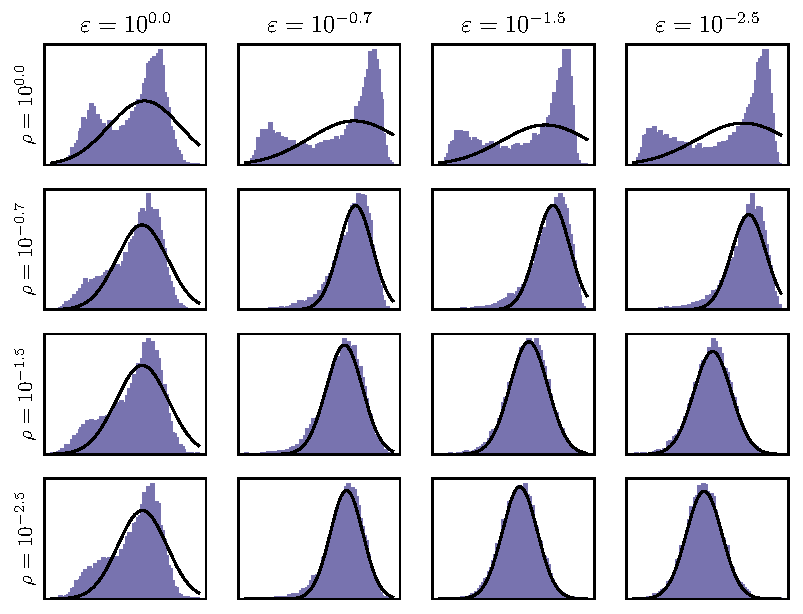
\includegraphics[width=\textwidth]{chp04_paper_numerics/figures/sine/selected_hists.pdf}
		\caption{Histograms of stochastic samples of \cref{eqn:sine_sde}, subject to the Gaussian initial condition \cref{eqn:num_gauss_init}, for varying initial uncertainty scale \(\rho\) and ongoing uncertainty scale \(\epsilon\).
			The distribution of the corresponding solution \cref{eqn:num_linear_sol} to the linearised equation is overlaid in black.}
		\label{fig:sine_hists}
	\end{center}
\end{figure}

In \Cref{fig:sine_hists}, we show histograms of \(N = 10000\) samples of the solution to nonlinear SDE \cref{eqn:sine_sde} and the corresponding probability density function of the linearised solution \cref{eqn:num_linear_sol}, for different combinations of \(\epsilon\) and \(\rho\).
Even when the ongoing noise is small, the nonlinearity of the drift term means that a large initial uncertainty results in a non-Gaussian distribution.
However, in situations where both the initial and ongoing uncertainties are small, the Gaussian solution to the linearised equation provides a reasonable approximation.
In the limit of both small initial (\(\rho \to 0\)) and small ongoing (\(\epsilon \to 0\)) uncertainty (towards the bottom right), we see that the distribution of the samples approach the Gaussian density of the linearisation solution, matching the understanding that the linearisation approximation is ``reasonable'' for small noise regimes.

Since the drift term is nonlinear and the noise is additive in \cref{eqn:sine_sde}, the bound predicted by \Cref{thm:main} has the form
\[
	\avg{\norm{y_t^{(\epsilon)} - l_t^{(\epsilon)}}^r} \leq D_1\!\left(r,t, K_{\nabla u}, K_\sigma\right)\epsilon^{2r} + M_{2r}D_2\!\left(r,t, K_{\nabla u}\right)\rho^{2r}.
\]
where we have taken \(K_{\nabla\nabla u} = 1\) and \(K_{\nabla\sigma} = 0\).
To numerically validate this bound under the Gaussian initial condition \cref{eqn:num_gauss_init}, define for \(r \geq 1\) the error measure
\begin{equation}
	E_r\!\left(\epsilon, \rho\right) \coloneqq \frac{1}{N}\sum_{i=1}^N{\norm{\hat{y}_{i}^{(\epsilon)} - \hat{l}_i^{(\epsilon)}}^r},
	\label{eqn:strong_err_mc_estimate}
\end{equation}
which is a Monte-Carlo estimator of the right-hand side of \cref{eqn:main_ineq}, where \(\hat{y}_1^{(\epsilon)},\dotsc, \hat{y}_N^{(\epsilon)}\) and \(\hat{l}_1^{(\epsilon)},\dotsc, \hat{l}_N^{(\epsilon)}\) are \(N\) numerical samples of the solutions to SDE \cref{eqn:sde_y} and the linearisation \cref{eqn:linear_sde_inform} respectively.

We directly validate the \emph{form} of the error bound (as a function of \(\epsilon\) and \(\rho\)) in \Cref{fig:sine_delta_eps_lines}, by computing \(E_1\) using samples for each pair of \(\epsilon\) and \(\rho\) values.
In \Cref{fig:sine_eps_lines}, we demonstrate the relationship between \(E_1\) and the ongoing uncertainty \(\epsilon\) for several different fixed values of \(\rho\), each corresponding to a different colour.
A least squares estimate of a line of best fit of the form \(E_1 = \beta_0 + \beta_1 \epsilon^2 \), for fixed coefficients \(\beta_0\) and \(\beta_1\), is fitted to the observed errors (in untransformed space) to verify the scaling of our bound in \Cref{thm:main}.
We see that the line of best fit accurately matches the observed values of \(E_1\), verifying that \(E_1\) is in fact scaling with \(\epsilon^2\) as predicted.
\Cref{fig:sine_delta_lines} provides a similar demonstration between \(E_1\) and the initial uncertainty \(\rho\), where now each colour corresponds to a different fixed value of \(\epsilon\).
We again fit lines of the form \(E_1 = \beta_0 + \beta_1 \rho^2\) to verify the scaling of the bound, and see that the lines match the observed values of \(E_2\).
Thus, we have also validated that \(E_1\) scales with \(\rho^2\), as expected from \Cref{thm:main}.

\begin{figure}
	\begin{center}
		\begin{subfigure}{\textwidth}
			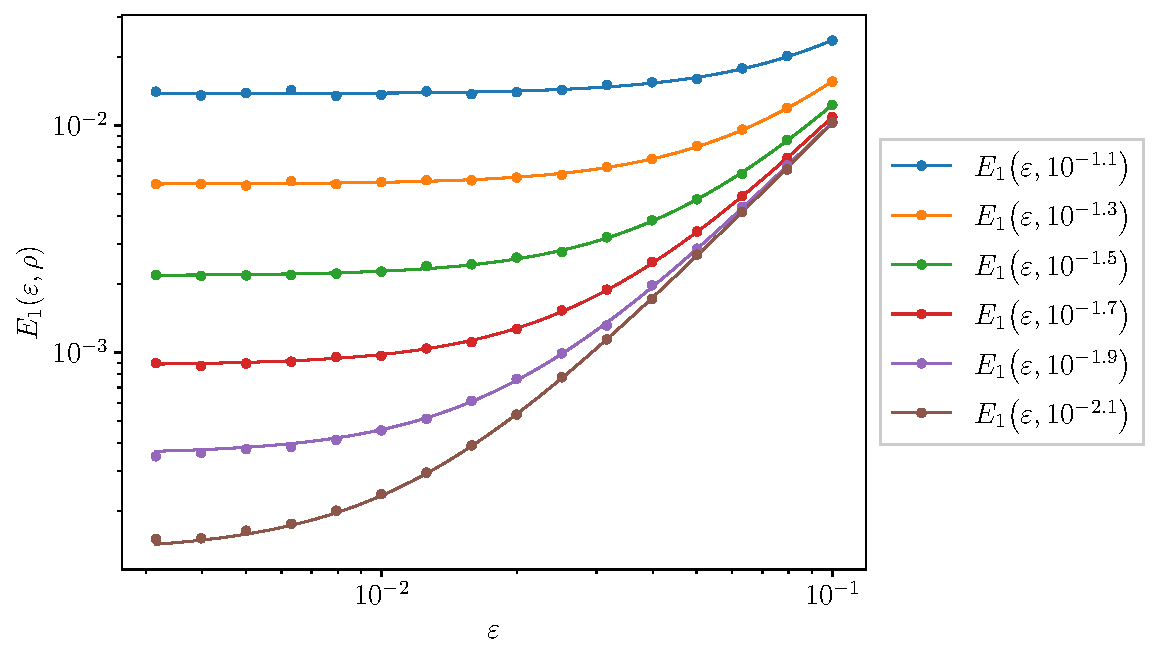
\includegraphics[width=\textwidth]{chp04_paper_numerics/figures/sine/str_err_eps_r_1.0_log.pdf}
			\caption{Estimates of the strong error (with \(r = 1\)) in linearising \cref{eqn:sine_sde} with \cref{eqn:sine_linear}, for varying ongoing uncertainty parameter \(\epsilon\).
				Each colour corresponds to a different value of the initial uncertainty parameter \(\rho\).
				A (least squares) line of best fit of the form \(\beta_0 + \beta_1 \epsilon^2\) is included in the corresponding colour.}
			\label{fig:sine_eps_lines}
		\end{subfigure}
		\begin{subfigure}{\textwidth}
			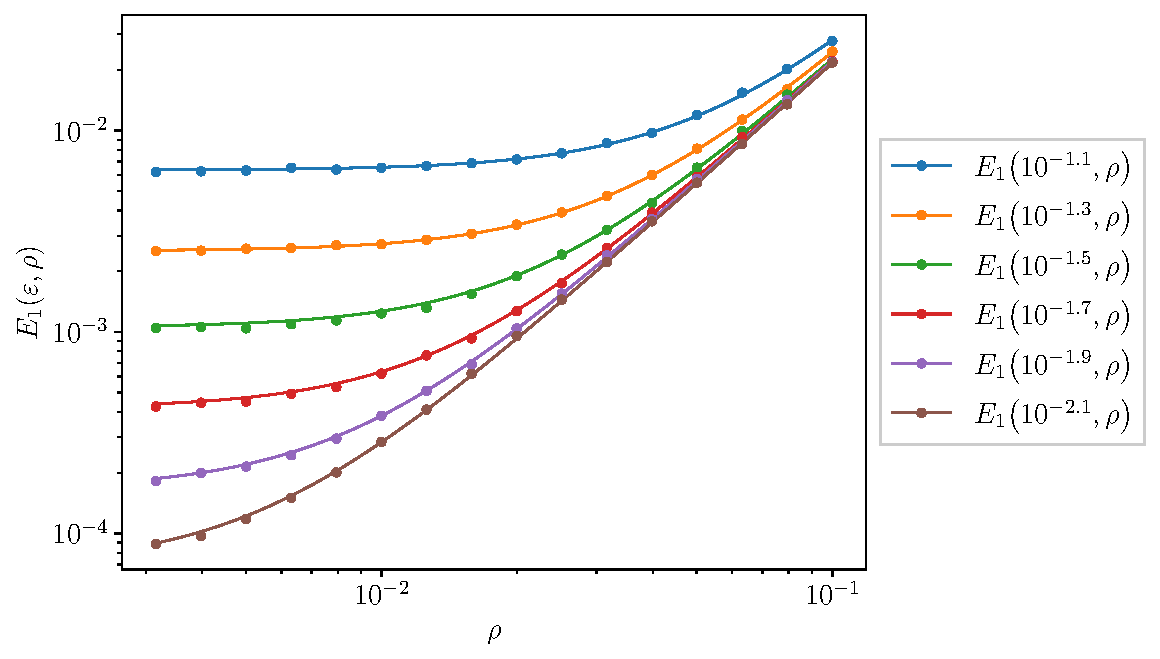
\includegraphics[width=\textwidth]{chp04_paper_numerics/figures/sine/str_err_rho_r_1.0_log.pdf}
			\caption{Estimates of the strong error (with \(r = 1\)) for varying initial uncertainty parameter \(\rho\).
				Each colour corresponds to a different value of the ongoing uncertainty parameter \(\epsilon\).
				A (least squares) line of best fit of the form \(\beta_0 + \beta_1 \rho^2\) is included in the corresponding colour.}
			\label{fig:sine_delta_lines}
		\end{subfigure}
		\caption{Validation of the theoretical bound predicted by \Cref{thm:main}, when \(r = 1\), on numerical realisations of the solution to the 1D example \cref{eqn:sine_sde}.}
		\label{fig:sine_delta_eps_lines}
	\end{center}
\end{figure}

\subsection{Linear dynamics, multiplicative noise}\label{sec:numerics_multiplicative}
Now consider the following SDE with multiplicative noise in 1D;
\begin{equation}
	\dif y_t^{(\epsilon)} = \frac12 y_t^{(\epsilon)}\dif t + \varepsilon \cos\!\left(y_t^{(\epsilon)}\right) \dif W_t.
	\label{eqn:1d_mult}
\end{equation}
The corresponding deterministic system is linear and has solution
\begin{equation}
	F_0^t\!\left(x_0\right) = \exp\!\left(\frac{t}{2}\right) x_0,
	\label{eqn:1d_mult_det_sol}
\end{equation}
with additional details provided in the supplementary materials.
As with the previous example in \Cref{sec:numerics_nonlinear}, we take the Gaussian initial condition \cref{eqn:num_gauss_init} with variance \(\rho^2\) and linearised \cref{eqn:1d_mult} about the initial mean \(\mu\).
The linearised equation is then
\begin{equation}
	\dif l_t^{(\epsilon)} = \frac12 l_t^{(\epsilon)}\dif t + \epsilon \cos\!\left(\exp\left(\frac{t}{2}\right)\mu\right) \dif W_t, \quad l_0^{(\epsilon)} \sim \Gauss{\mu, \rho^2},
	\label{eqn:1d_mult_linear}
\end{equation}
with Gaussian solution \cref{eqn:num_linear_sol}.
We take the initial point \(\mu = 2\) and consider the solutions at time \(t = 1\).
To generate numerical realisations of the solutions to \cref{eqn:1d_mult} and \cref{eqn:1d_mult_linear} with the same realisations of \(W_t\), we use the same set-up as in the previous example.

In \Cref{fig:sine_hists}, we show histograms of \(N = 10000\) samples of the multiplicative noise SDE \cref{eqn:1d_mult} and the corresponding probability density function of the linearised solution, for different combinations of \(\epsilon\) and \(\rho\).
We again see that in the limit of both small initial and small ongoing uncertainty (towards the bottom right), we see that the distribution of the samples approach the Gaussian density of the linearisation solution.

\begin{figure}
	\begin{center}
		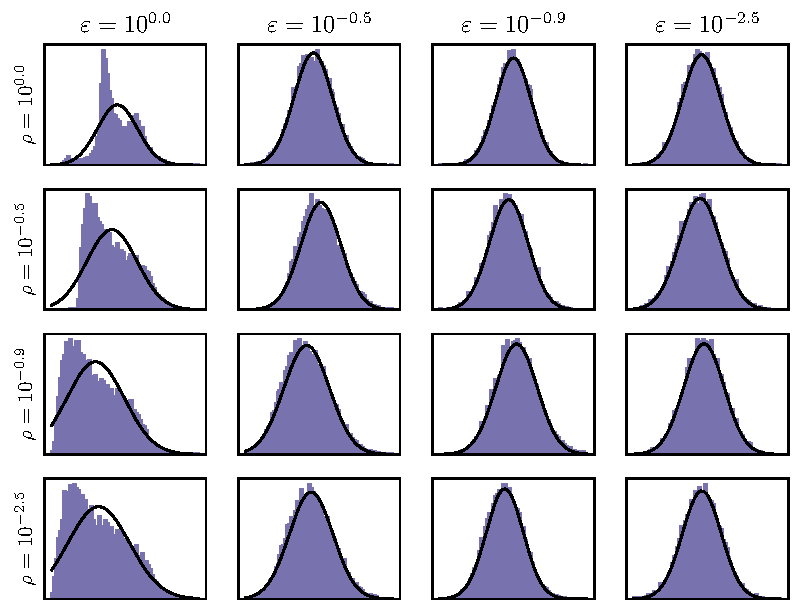
\includegraphics[width=\textwidth]{chp04_paper_numerics/figures/multiplicative/selected_hists.pdf}
		\caption{The same arrangement as \Cref{fig:sine_hists}, but for the 1D multiplicative noise SDE \cref{eqn:1d_mult}.}
		\label{fig:1d_mult_hists}
	\end{center}
\end{figure}

Since the drift term is linear and the noise multiplicative in \cref{eqn:1d_mult}, the bound predicted by \Cref{thm:main} has the form
\[
	\avg{\norm{y_t^{(\epsilon)} - l_t^{(\epsilon)}}^r} \leq D_1\!\left(r,t, K_{\nabla u}, K_\sigma\right)\epsilon^{2r} + M_{r}D_3\!\left(r,t, K_{\nabla u}\right)\epsilon^r\rho^{r},
\]
where we have \(K_{\nabla\nabla u} = 0\) and \(K_{\nabla\sigma} = 1\).
In \Cref{fig:multiplicative_delta_eps_lines}, we again validate the form of this bound (for \(r = 1\); results for additional values of \(r\) are provided in the supplementary material) by approximating the left-hand side with \(E_1\) computed from realisations of the solution to \cref{eqn:1d_mult} and the linearisation \cref{eqn:1d_mult_linear}.
For each fixed value of the initial uncertainty \(\rho\), in \Cref{fig:multiplicative_eps_lines}, we fit a line of best fit of the form \(\beta_1 \epsilon + \beta_2 \epsilon^2\) to validate that the strong error scales as predicted.
Similarly, in \Cref{fig:multiplicative_eps_lines} we fit a line of best fit of the form \(\beta_0 + \beta_1 \rho\) and confirm that the linearisation error follows this scaling.

\begin{figure}
	\begin{center}
		\begin{subfigure}{\textwidth}
			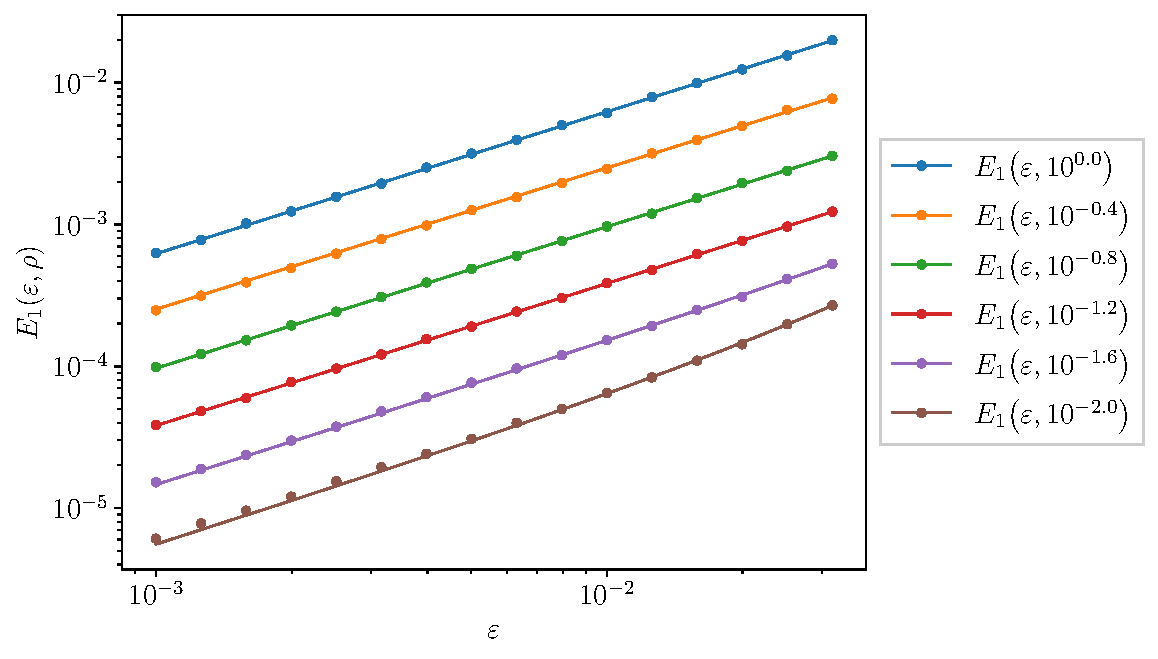
\includegraphics[width=\textwidth]{chp04_paper_numerics/figures/multiplicative/str_err_eps_r_1.0_log.pdf}
			\caption{Estimates of the strong order (with \(r = 1\)) for varying ongoing uncertainty parameter \(\epsilon\).
				Each colour corresponds to a different value of the initial uncertainty parameter \(\rho\).
				A (least squares) line of best fit of the form \(\beta_1 \epsilon + \beta_2 \epsilon^2\) is included in the corresponding colour.}
			\label{fig:multiplicative_eps_lines}
		\end{subfigure}
		\begin{subfigure}{\textwidth}
			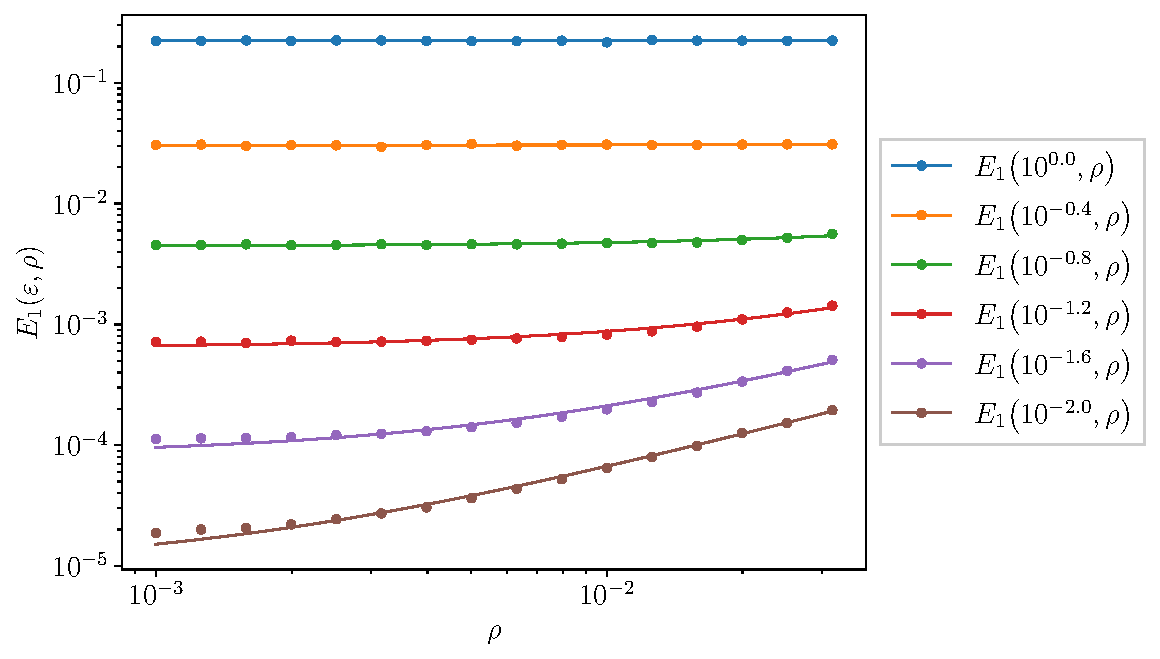
\includegraphics[width=\textwidth]{chp04_paper_numerics/figures/multiplicative/str_err_rho_r_1.0_log.pdf}
			\caption{Estimates of the strong order (with \(r = 1\)) for varying initial uncertainty parameter \(\rho\).
				Each colour corresponds to a different value of the ongoing uncertainty parameter \(\epsilon\).
				A (least squares) line of best fit of the form \(\beta_0 + \beta_1 \rho\) is included in the corresponding colour.}
			\label{fig:multiplicative_delta_lines}
		\end{subfigure}
		\caption{Validation of the theoretical bound predicted by \Cref{thm:main}, when \(r = 1\), on numerical realisations of the solution to the 1D example \cref{eqn:1d_mult}.}
		\label{fig:multiplicative_delta_eps_lines}
	\end{center}
\end{figure}

\subsection{Fixed initial condition}\label{sec:numerics_2d}
In this example, we consider a two-dimensional model and a fixed initial condition, to validate the results presented in \Cref{sec:theory_fixed}.
Following the example in Chapter 5 of \citet{SamelsonWiggins_2006_LagrangianTransportGeophysical}, we consider an unsteady meandering jet in two dimensions, which may serve as an idealised model of geophysical Rossby waves \citep{Pierrehumbert_1991_ChaoticMixingTracer}.
The velocity field for \(y \equiv \left(y_1, y_2\right)^{\T}\) is given by
\begin{equation}
	u\!\left(y, t\right) = \begin{bmatrix}
		c - A\sin\!\left(Ky_1\right)\cos\!\left(y_2\right) + \oldepsilon_{\mathrm{mj}} l_1\sin\!\left(k_1\left(y_1 - c_1 t\right)\right)\cos\!\left(l_1 y_2\right) \\
		AK\cos\!\left(Ky_1\right)\sin\!\left(y_2\right) + \oldepsilon_{\mathrm{mj}} k_1\cos\!\left(k_1\left(y_1 - c_1t\right)\right)\sin\!\left(l_1 y_2\right)
	\end{bmatrix}.
	\label{eqn:jet_ex}
\end{equation}
The velocity field describes a kinematic travelling wave with deterministic oscillatory perturbations in a co-moving frame.
Here, \(A\) is the amplitude and \(c\) is the phase speed of the primary wave, and \(K\) is the wavenumber in the \(y_1\)-direction.
The oscillatory perturbation has amplitude \(\oldepsilon_{\mathrm{mj}}\), phase speed \(c_1\) (in the co-moving frame), and wavenumbers \(k_1\) and \(l_1\) in the \(y_1\)- and \(y_2\)-directions respectively.
Throughout, we take the parameter values \(c = 0.5\), \(A = 1\), \(K = 4\), \(l_1 = 2\), \(k_1 = 1\), \(c_1 = \pi\), and \(\oldepsilon_{\mathrm{mj}} = 0.3\).
For these values, the flow consists of a meandering jet with vortex structures within the meanders, and a chaotic zone which influences the fluid transfer between the jet and the vortices.

We introduce multiplicative noise by considering stochastic perturbations to the phase speed \(c\) and the primary amplitude \(A\), which we model with the respective components of a \(2\)-dimensional Wiener process \(W_t = \left(W_t^{(1)}, W_t^{(2)}\right)^{\T}\).
Then, we specify the diffusion term as
\begin{equation}
	\sigma\!\left(y,t\right) = \begin{bmatrix}
		1 & \sin\!\left(Ky_1\right)\cos\!\left(y_2\right)  \\
		0 & K\cos\!\left(Ky_1\right)\sin\!\left(y_2\right)
	\end{bmatrix}.
	\label{eqn:jet_ex_sigma}
\end{equation}


We consider the fixed initial condition \(x_0 = \left(0, 1\right)\) and the prediction of the model at time \(t = 1\).
We then consider a linearisation of the SDE about the deterministic trajectory \(F_0^t\!\left(x_0\right)\), where \(F_0^t\) is the deterministic flow map corresponding to the vector field \cref{eqn:jet_ex}.
To compute the Gaussian distribution \cref{eqn:linear_gauss_sol} of the linearised solution, we again solve \cref{eqn:pi_ode} numerically with initial condition \(\Sigma_0^t\!\left(x_0\right) = O\).
Specifically, \cref{eqn:pi_ode} is solved jointly with the deterministic state equation \cref{eqn:ode_det} using the hybrid method proposed by \citet{Mazzoni_2008_ComputationalAspectsContinuous}.
This hybrid method combines a Taylor-Heun approximation with a Gauss-Legendre one and ensures that the numerical solution of the covariance equation is symmetric and positive semi-definite while maintaining both accuracy and computational efficiency.


\Cref{fig:y_hists} shows the resulting simulations of \(y_t^{(\epsilon)}\) for four different values of \(\epsilon\).
The realisations are binned as a histogram and bin counts are normalised, to provide an empirical estimate of the probability density function of \(y_t^{(\epsilon)}\).
Superimposed (in solid black) are the first, second and third standard-deviation contours of the probability density function of the Gaussian distribution that solves the linearised equation.
The first three standard-deviation levels of the \(2\times 2\) sample covariance matrix of the realisations of \(y_t^{(\epsilon)}\), are also overlaid (in dashed blue).
As \(\epsilon\) decreases towards \(0\), the samples increasingly resemble a Gaussian distribution, and both the mean and covariance coincide with the corresponding limits.

\begin{figure}
	\begin{center}
		\begin{subfigure}{0.49\textwidth}
			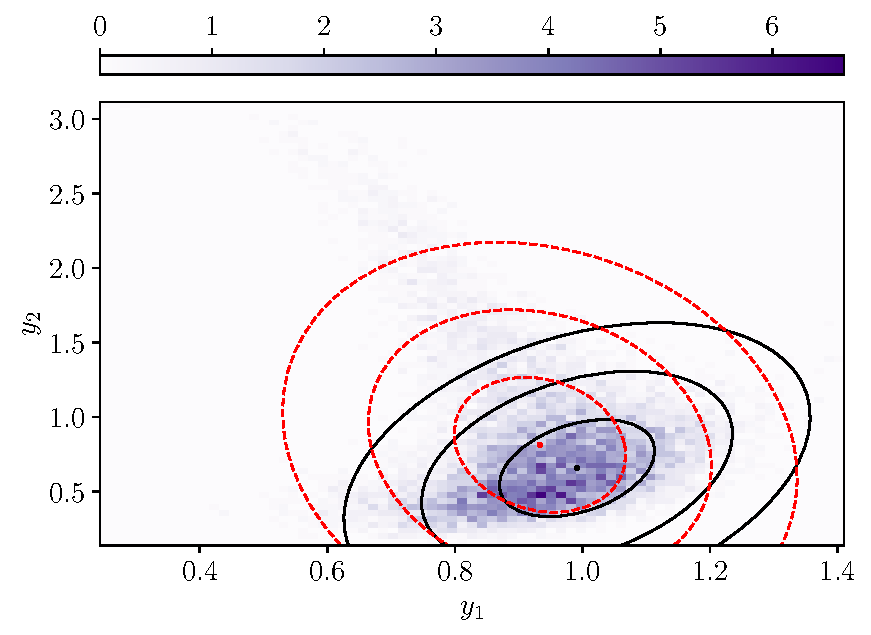
\includegraphics[width=\textwidth]{chp04_paper_numerics/figures/rossby/hist_0.1.pdf}
			\caption{\(\epsilon = 10^{-1}\)}
			\label{fig:y_hists_a}
		\end{subfigure}
		\begin{subfigure}{0.49\textwidth}
			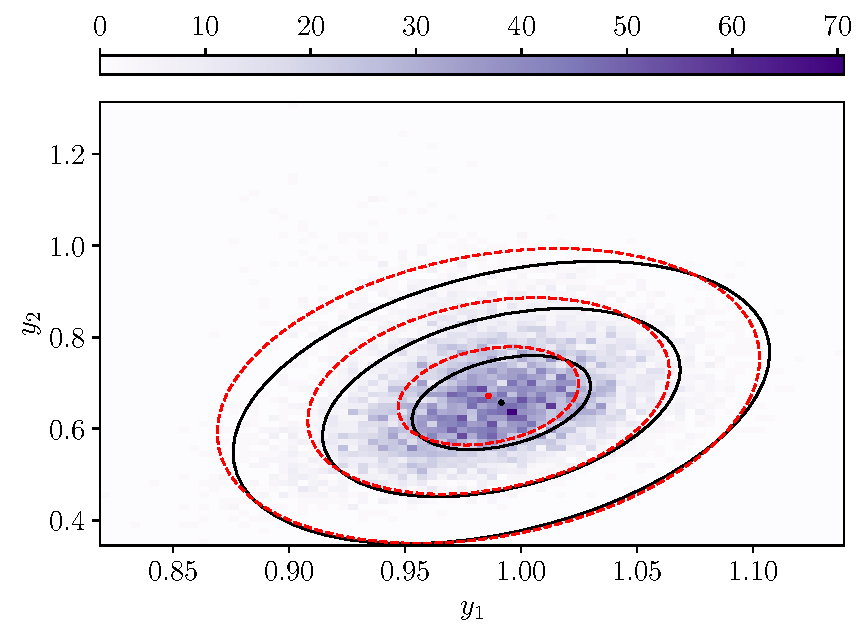
\includegraphics[width=\textwidth]{chp04_paper_numerics/figures/rossby/hist_0.03162277660168379.pdf}
			\caption{\(\epsilon = 10^{-1.5}\)}
			\label{fig:y_hists_b}
		\end{subfigure}
		\begin{subfigure}{0.49\textwidth}
			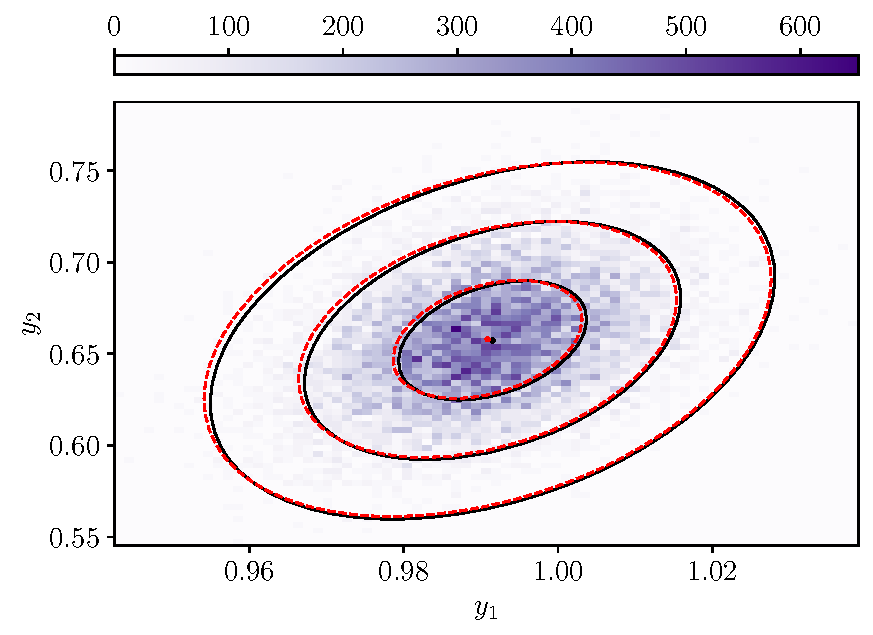
\includegraphics[width=\textwidth]{chp04_paper_numerics/figures/rossby/hist_0.010000000000000002.pdf}
			\caption{\(\epsilon = 10^{-2}\)}
			\label{fig:y_hists_c}
		\end{subfigure}
		\begin{subfigure}{0.49\textwidth}
			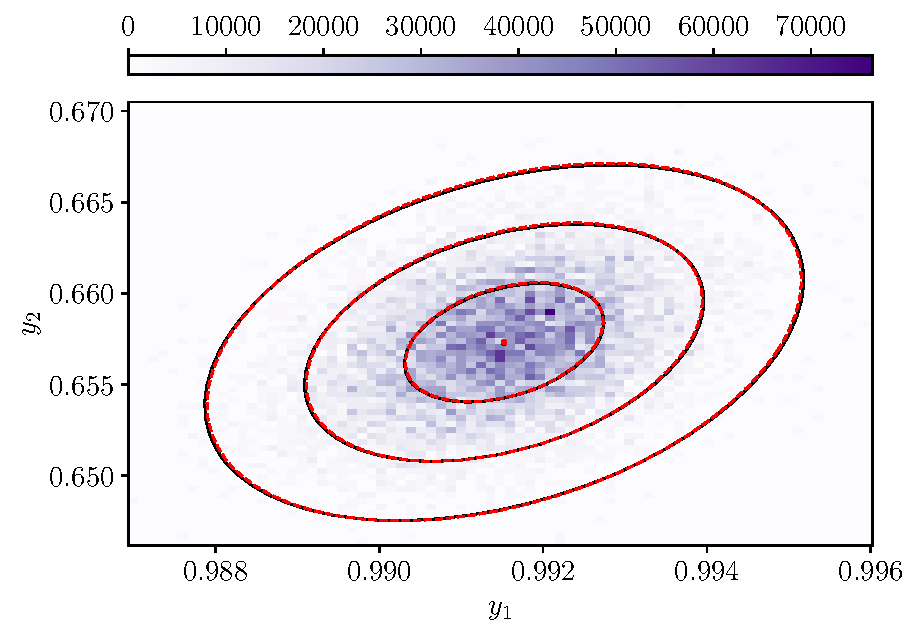
\includegraphics[width=\textwidth]{chp04_paper_numerics/figures/rossby/hist_0.001.pdf}
			\caption{\(\epsilon = 10^{-3}\)}
			\label{fig:y_hists_d}
		\end{subfigure}
		\caption{Histograms of \(y_t^{(\epsilon)}\) from direct simulation of the SDE with drift \cref{eqn:jet_ex} and diffusivity \cref{eqn:jet_ex_sigma} subject to the fixed initial condition, for four different \(\epsilon\) values.
		Overlaid in black are contours of the Gaussian solution \cref{eqn:linear_gauss_sol} of the linearised SDE \cref{eqn:linear_sde_inform}, which correspond to the first three standard deviation levels centred at the mean \(F_0^t(x)\).
		In dashed blue are corresponding contours computed from the sample covariance matrix of the realisations.
		}
		\label{fig:y_hists}
	\end{center}
\end{figure}

For a fixed initial condition, \cref{eqn:main_ineq} predicts that the expected distance between the original SDE solution and that of a linearisation satisfies
\[
	\avg{\norm{y_t^{(\epsilon)} - l_t^{(\epsilon)}}^r} \leq \left(K_{\nabla\nabla u} + K_{\nabla\sigma}\right)D_1\!\left(r,t, K_{\nabla u}, K_\sigma\right)\epsilon^{2r}.
\]
To numerically estimate the left-hand side of \cref{eqn:main_ineq}, we again use a Monte-Carlo estimator;
\[
	E_r\!\left(\epsilon\right) \coloneqq \frac{1}{N}\sum_{i=1}^N{\norm{\hat{y}_i^{(\epsilon)} - \hat{l}_i^{(\epsilon)}}^r}.
\]
For \(r = 1,2,3,4\), \(E_r\!\left(\epsilon\right)\) is shown (in a logarithmic scale) for decreasing values of \(\epsilon\) in \Cref{fig:gamma_z_valid}.
\Cref{thm:main} predicts that \(\log_{10}\left(E_r\!\left(\epsilon\right)\right)\) should decay linearly with a slope greater than \(2r\) as \(\epsilon\) decreases to zero.
The least squares lines of best fit for each value of \(r\) in \Cref{fig:gamma_z_valid} show this behaviour, and are therefore consistent with \Cref{thm:main}.

\begin{figure}
	\begin{center}
		\begin{subfigure}{0.49\textwidth}
			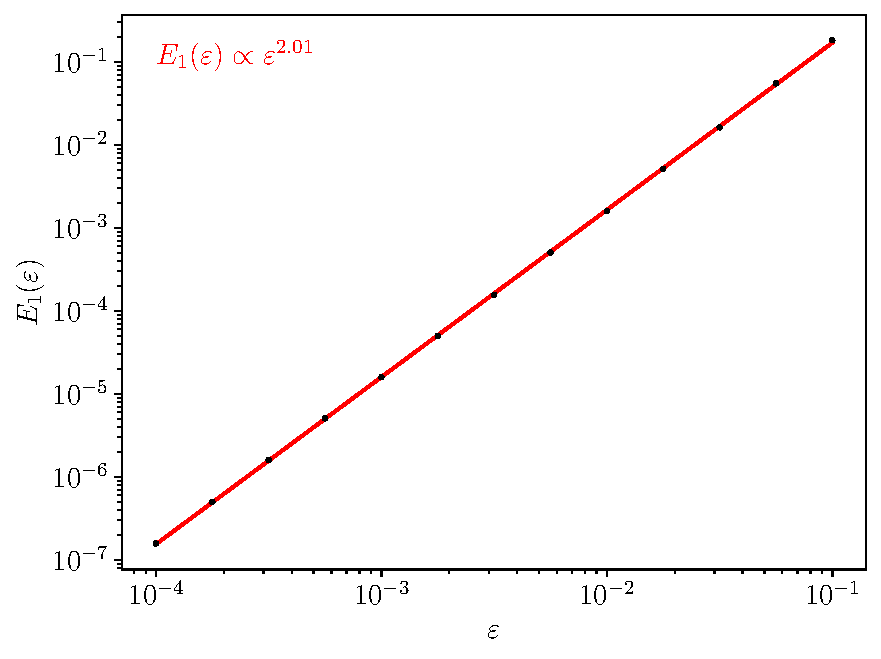
\includegraphics[width=\textwidth]{chp04_paper_numerics/figures/rossby/str_err_r_1.0.pdf}
			\caption{\(r = 1\) (mean)}
			\label{fig:gamma_z_valid_1}
		\end{subfigure}
		\begin{subfigure}{0.49\textwidth}
			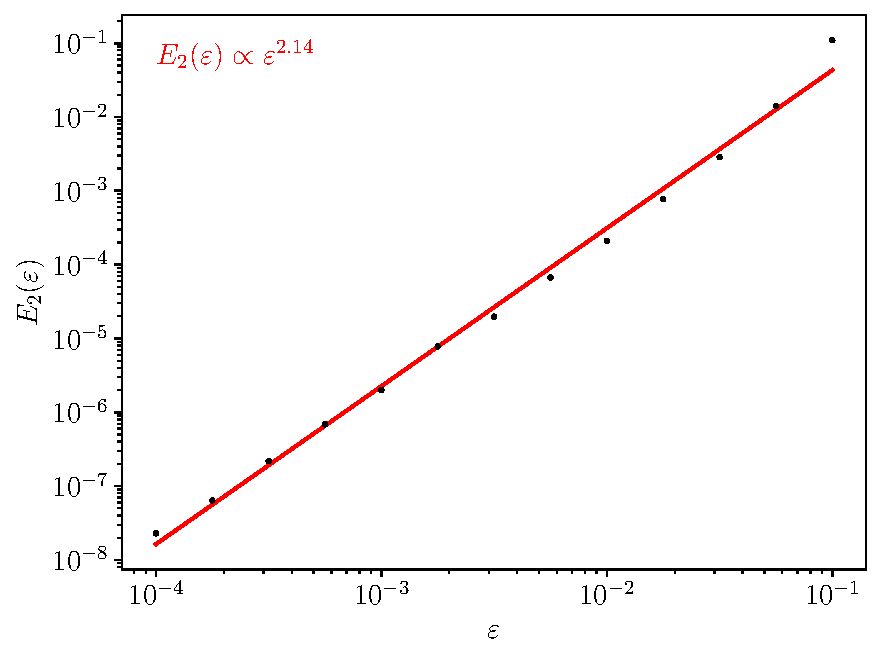
\includegraphics[width=\textwidth]{chp04_paper_numerics/figures/rossby/str_err_r_2.0.pdf}
			\caption{\(r = 2\) (variance)}
			\label{fig:gamma_z_valid_2}
		\end{subfigure}
		\begin{subfigure}{0.49\textwidth}
			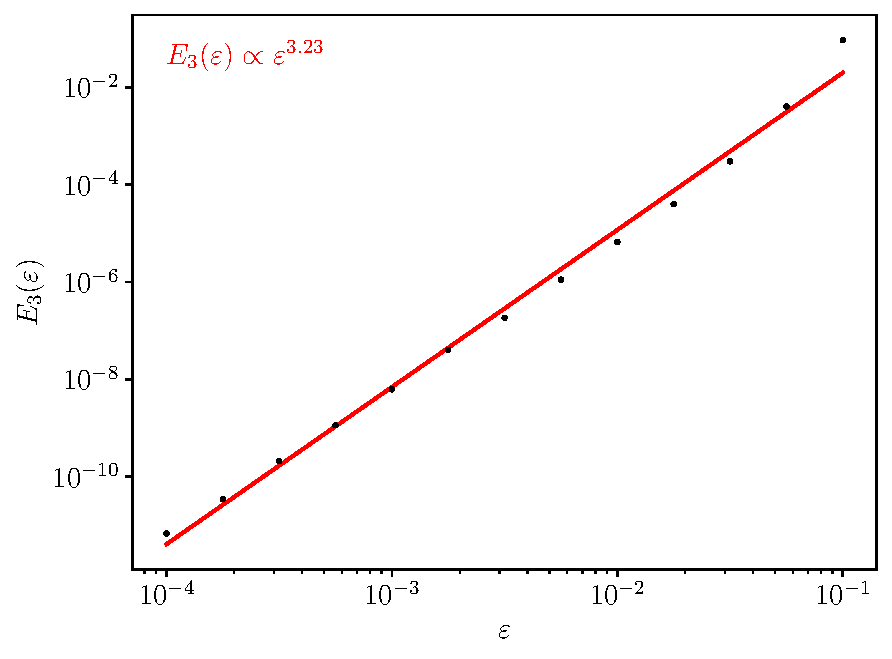
\includegraphics[width=\textwidth]{chp04_paper_numerics/figures/rossby/str_err_r_3.0.pdf}
			\caption{\(r = 3\) (skewness)}
			\label{fig:gamma_z_valid_3}
		\end{subfigure}
		\begin{subfigure}{0.49\textwidth}
			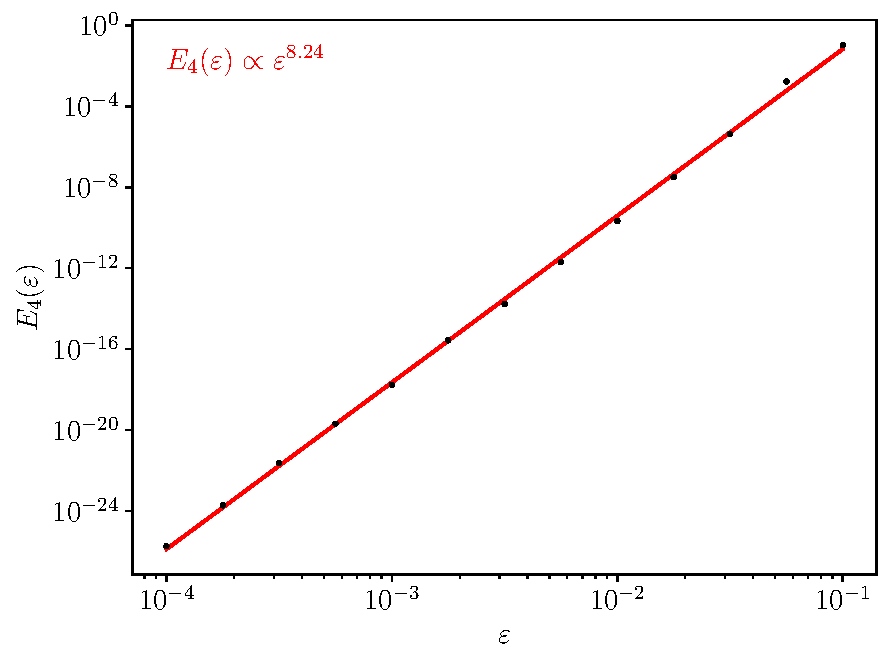
\includegraphics[width=\textwidth]{chp04_paper_numerics/figures/rossby/str_err_r_4.0.pdf}
			\caption{\(r = 4\) (kurtosis)}
			\label{fig:gamma_z_valid_4}
		\end{subfigure}

		\caption{Validation of \Cref{thm:main}, by plotting the sample \(r\)th raw moment distance (the error metric \(E_r(\epsilon)\)) between \(10000\) realisations of the meandering jet SDE and a corresponding linearisation, for decreasing values of \(\epsilon\).
			A line of best fit (in red) is placed on each, and the resulting slope indicated.}
		\label{fig:gamma_z_valid}
	\end{center}
\end{figure}


\section{Computing stochastic sensitivity} \label{sec:comput_s2}
In this section, we illustrate the computability of stochastic sensitivity as described in \Cref{thm:s2_calculation}.

\subsection{In 2-dimensions}\label{sec:compute_s2_2d}

\begin{figure}
	\begin{center}
		\begin{subfigure}{\textwidth}
			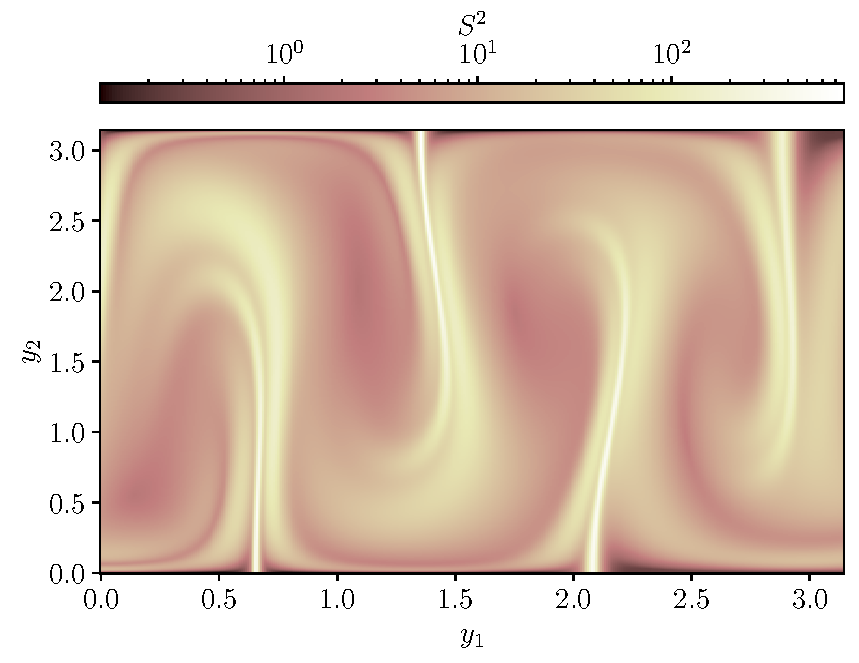
\includegraphics[width=0.49\textwidth]{chp04_paper_numerics/figures/rossby/S2_zero_0.3}
			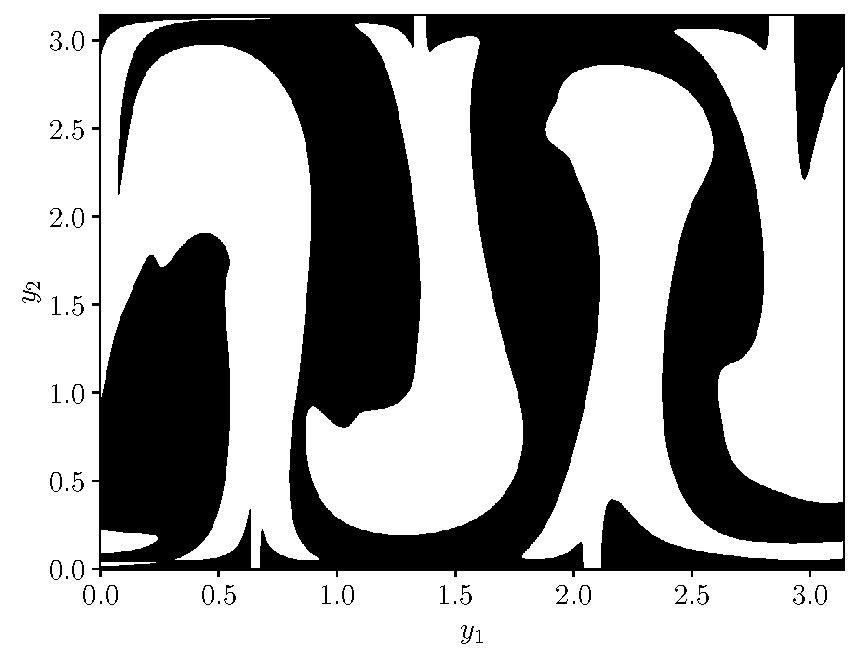
\includegraphics[width=0.49\textwidth]{chp04_paper_numerics/figures/rossby/S2_robust_0.3}
			\caption{\(\oldepsilon_{\mathrm{mj}} = 0.3\)}
			\label{fig:s2_field_0.3}
		\end{subfigure}
		\begin{subfigure}{\textwidth}
			\includegraphics[width=0.49\textwidth]{chp04_paper_numerics/figures/rossby/s2_zero_1.0}
			\includegraphics[width=0.49\textwidth]{chp04_paper_numerics/figures/rossby/s2_robust_1.0}
			\caption{\(\oldepsilon_{\mathrm{mj}} = 1.0\)}
			\label{fig:s2_field_1.0}
		\end{subfigure}
		\caption{(Left) The \(S^2\) field of the meandering jet flow \cref{eqn:jet_ex} over the time interval \([0,1]\), for two different sets of parameters with qualitatively different behaviour.
			The \(S^2\) value for each initial condition is computed directly as the operator norm of the covariance matrix \(\Sigma_0^1\!\left(x_0\right)\), as per \cref{eqn:s2_calculation}.
			(Right) Robust sets extracted from the stochastic sensitivity fields, by taking the initial conditions with a stochastic sensitivity value about a threshold of \(10\).}
		\label{fig:ex_jet_s2_field}
	\end{center}
\end{figure}

We again consider the meandering jet \cref{eqn:jet_ex} with multiplicative noise described by \cref{eqn:jet_ex_sigma}.
We take the same choice of parameters as in \cref{sec:numerics_2d}, except for the perturbation amplitude \(\oldepsilon_{\mathrm{mj}}\) which is varied to obtain qualitatively different behaviour in the system.
For each initial condition in a \(400 \times 400\) uniform grid on \(\left[0, \pi\right] \times \left[0, \pi\right]\), the \(S^2\) value is calculated using \cref{eqn:s2_calculation}.
\Cref{fig:ex_jet_s2_field} shows the resulting \(S^2\) field from time \(0\) to \(t = 1\), for two different values of \(\oldepsilon_{\mathrm{mj}}\).
We also extract robust sets from each stochastic sensitivity field, by highlighting in cyan on the right side of \Cref{fig:ex_jet_s2_field} those initial conditions with a stochastic sensitivity value less than the specified threshold of 10.
When \(\oldepsilon_{\mathrm{mj}} = 0.3\) (\Cref{fig:s2_field_0.3}), the \(S^2\) field is largest in the elongated gyre regions outside of the meandering jet, where the flow exhibits chaotic behaviour \citep{Pierrehumbert_1991_ChaoticMixingTracer} and we accordingly expect larger uncertainty due to the model dynamics.
As a region of small \(S^2\) value, the meandering jet emerges as a robust set, consisting of initial points whose eventual fate is significantly more certain than in other regions.
When \(\oldepsilon_{\mathrm{mj}} = 1.0\) (\Cref{fig:s2_field_1.0}), the deterministic flow is dominated by oscillatory perturbation, which further increases the chaotic nature of the solving trajectories and the boundaries between the gyres and the meandering jet are no longer distinguishable \citep{Crocker_2021_LagrangianCoherentData}.
Rotational eddies begin to dominate the flow and we see this reflected in the stochastic sensitivity field in \Cref{fig:s2_field_1.0}: the eddies exhibit a smaller stochastic sensitivity, as even under stochasticity trajectories are inclined to remain within them.
The resulting robust sets highlight these eddies.\lb{Don't love this analysis, but almost there. Reconsider on next read through.}

% \begin{figure}
% 	\begin{center}
% 		\begin{subfigure}{0.49\textwidth}
% 			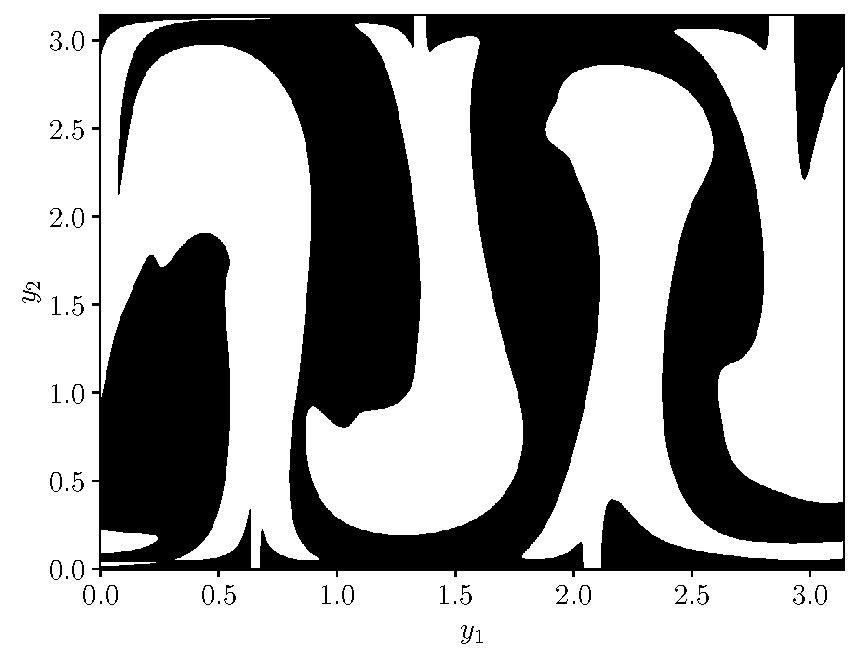
\includegraphics[width=\textwidth]{chp04_paper_numerics/figures/rossby/S2_robust_0.3.pdf}
% 			\caption{\(\oldepsilon_{\mathrm{mj}} = 0.3\), \(R = 10\)}
% 		\end{subfigure}
% 		\begin{subfigure}{0.49\textwidth}
% 			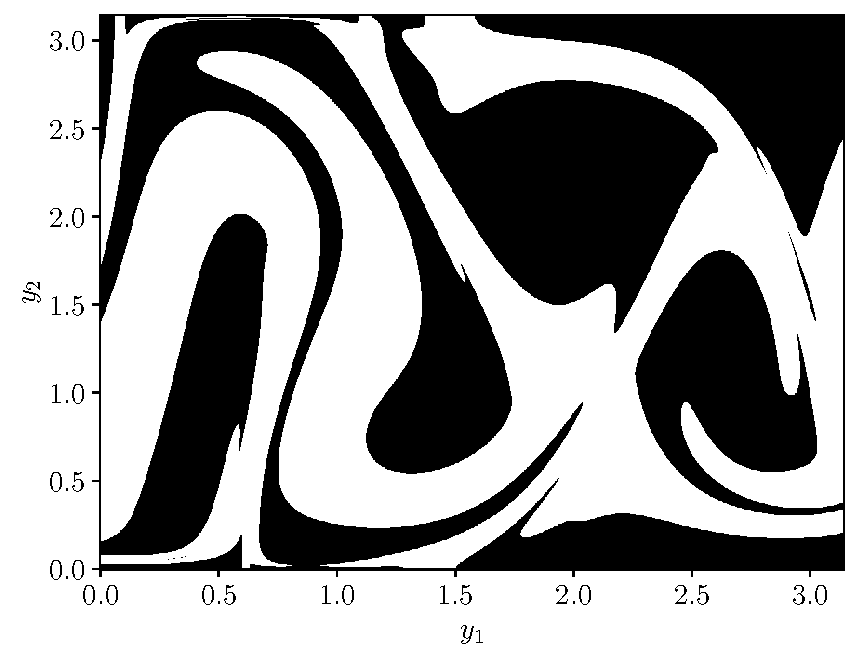
\includegraphics[width=\textwidth]{chp04_paper_numerics/figures/rossby/S2_robust_1.0.pdf}
% 			\caption{\(\oldepsilon_{\mathrm{mj}} = 1.0\), \(R = 10\)}
% 		\end{subfigure}
% 		\caption{Robust sets extracted from the stochastic sensitivity fields in \Cref{fig:ex_jet_s2_field}, by taking the initial conditions with a stochastic sensitivity value above a specified threshold \(R\). }
% \td{Use cyan for robust sets, to be consistent with later results.}
% 		\label{fig:ex_jet_robust}
% 	\end{center}
% \end{figure}

% The stochastic sensitivity field can highlight Lagrangian coherent structures within the flow, by identifying regions of the flow with a relatively small uncertainty, as measured by a \emph{single} number for each initial condition.
% Subsets of the spatial domain corresponding to coherent structures can be extracted, e.g.\ by taking a threshold on \(S^2\) as described in the original work \citep{Balasuriya_2020_StochasticSensitivityComputable}; further examples of coherent structure extraction with stochastic sensitivity on both toy models and real data can be found in \citet{Balasuriya_2020_StochasticSensitivityComputable} and \citet{BadzaEtAl_2023_HowSensitiveAre}.
% Here, we demonstrate the extraction of coherent structures in \Cref{fig:ex_jet_robust} using a threshold of \(R\).
% The resulting subsets of the domain in cyan reflect our conclusions from the stochastic sensitivity field itself; when \(\epsilon_{\mathrm{mj}} = 0.3\) the meandering jet



% \begin{figure}
% 	\begin{center}
% 		\begin{subfigure}{0.49\textwidth}
% 			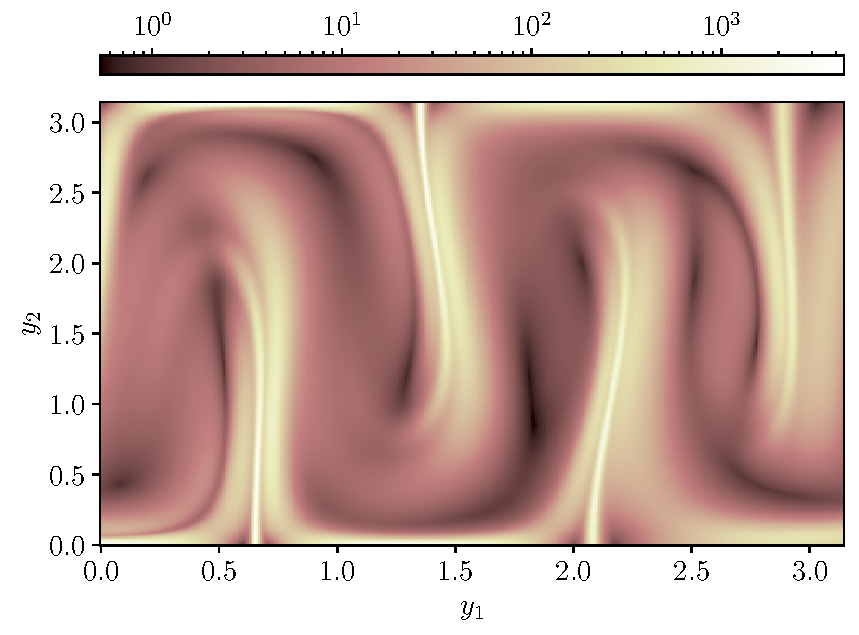
\includegraphics[width=\textwidth]{chp04_paper_numerics/figures/rossby/ftle_0.3.pdf}
% 			\caption{\(\oldepsilon_{\mathrm{mj}} = 0.3\)}
% 		\end{subfigure}
% 		\begin{subfigure}{0.49\textwidth}
% 			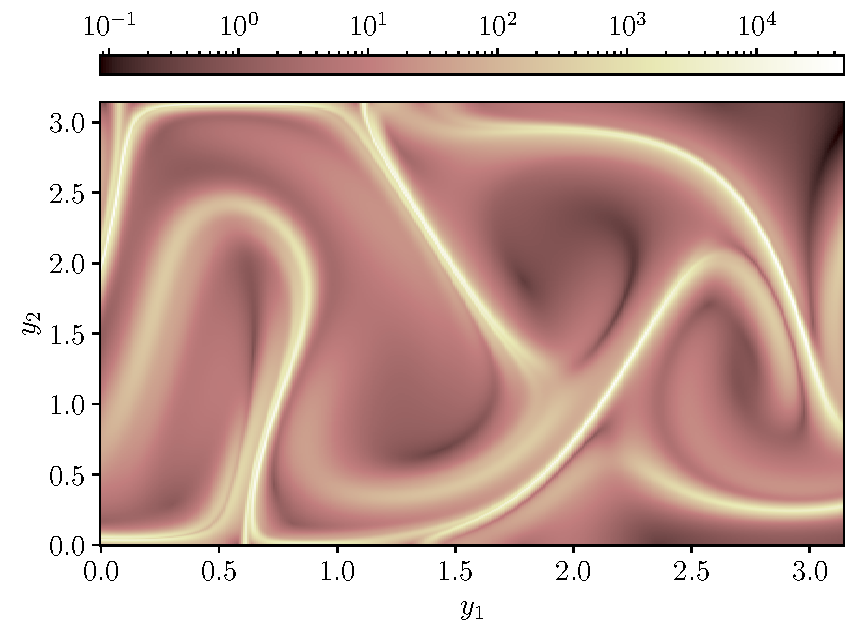
\includegraphics[width=\textwidth]{chp04_paper_numerics/figures/rossby/ftle_1.0.pdf}
% 			\caption{\(\oldepsilon_{\mathrm{mj}} = 1.0\)}
% 		\end{subfigure}
% 		\caption{The finite-time Lyapunov exponent field of the meandering jet flow \cref{eqn:jet_ex} over the time \([0,1]\), for two different values of \(\oldepsilon_{\mathrm{mj}}\).
% 			These fields should be compared with the corresponding stochastic sensitivity fields in \Cref{fig:ex_jet_s2_field}.}
% 	\end{center}
% 	\label{fig:ex_jet_ftle}
% \end{figure}



% In this example, the stochastic sensitivity and FTLE fields show strong similarities, supporting the claims in \Cref{sec:ftle_s2_connection} that stochastic sensitivity can be considered a generalisation of the FTLE.
% The two fields are quantifying different aspects of the flow, however, and so can show differences; such examples are available in \citet{Balasuriya_2020_StochasticSensitivityComputable} (see Figure 3.7) and \citet{BadzaEtAl_2023_HowSensitiveAre} (compare Figures 1 and 5, and Figures 11 and 15).

% To highlight the differences between the stochastic sensitivity field and the finite-time Lyapunov exponent, here we provide a brief and contrived example in which multiplicative noise has a substantial impact on the dynamical behaviour of the system.
% Following the example of \citet{BalasuriyaGottwald_2018_EstimatingStableUnstable}, consider the two-dimensional velocity field
% \begin{equation*}
% 	u\!\left(y, t\right) = \begin{bmatrix}
% 		-4y_1 + y_1^2 \\
% 		3y_2 - y_2^3
% 	\end{bmatrix},
% \end{equation*}
% To introduce multiplicative noise, we take the diffusivity
% \[
% 	\sigma\!\left(y,t\right) = \begin{bmatrix}
% 		1       & 0                                       \\
% 		y_2 - 1 & 3\sin\!\left(2\pi y_1\right)e^{-0.8y_1}
% 	\end{bmatrix},
% \]
% which in particular ensures a non-trivial spatial dependence along the stable manifold of interest.





% \begin{figure}
% 	\begin{center}
% 		\begin{subfigure}{0.49\textwidth}
% 			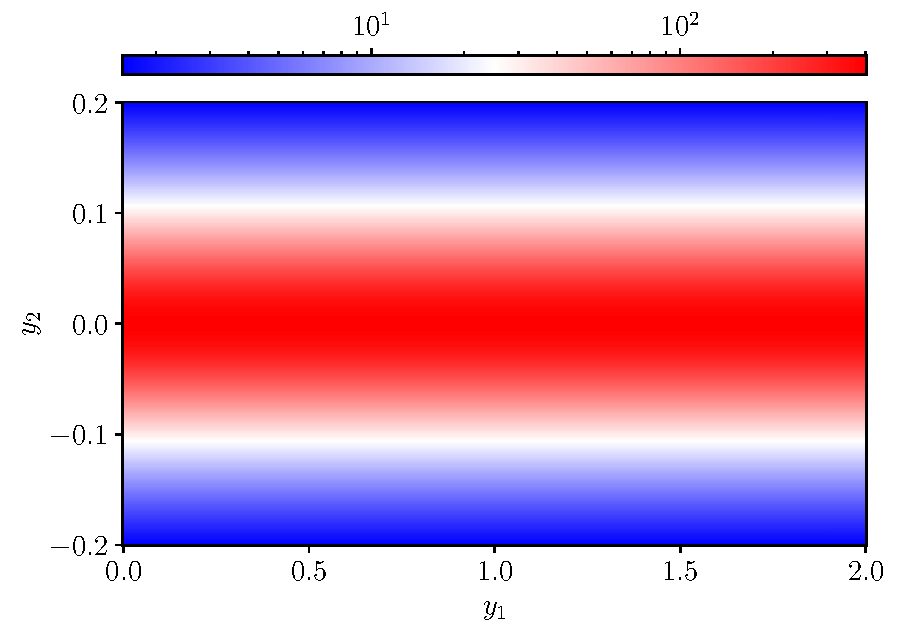
\includegraphics[width=\textwidth]{chp04_paper_numerics/figures/unstable/ftle.pdf}
% 			\caption{FTLE}
% 			\label{fig:s2_ftle_ftle}
% 		\end{subfigure}
% 		\begin{subfigure}{0.49\textwidth}
% 			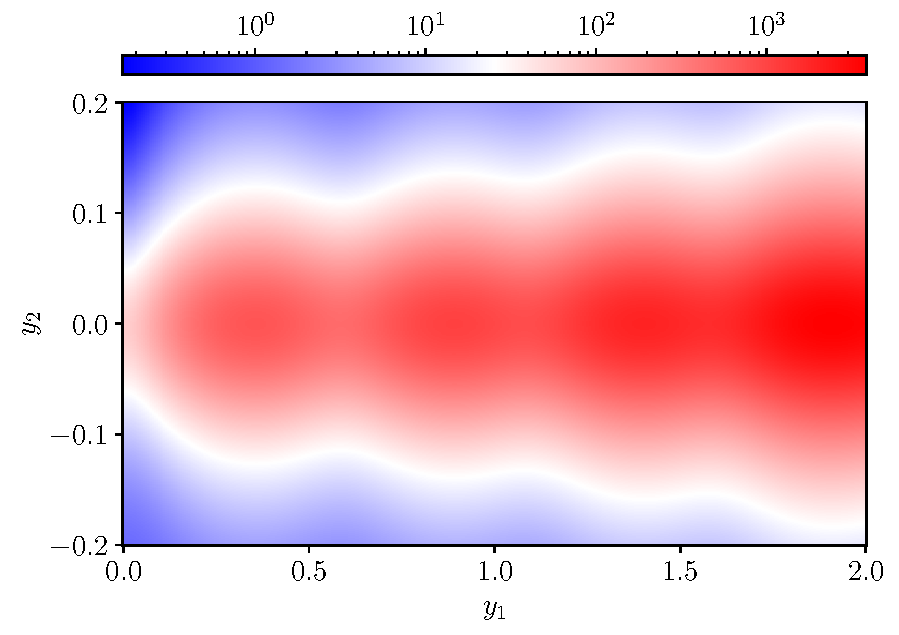
\includegraphics[width=\textwidth]{chp04_paper_numerics/figures/unstable/S2_zero.pdf}
% 			\caption{\(S^2\) with fixed initial condition.}
% 			\label{fig:s2_ftle_ftle}
% 		\end{subfigure}		\begin{subfigure}{0.49\textwidth}
% 			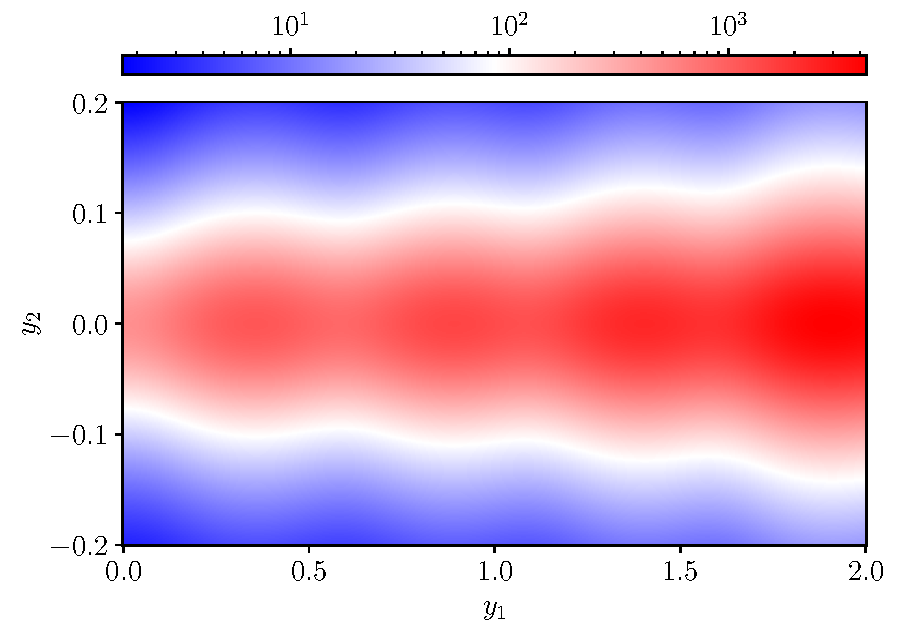
\includegraphics[width=\textwidth]{chp04_paper_numerics/figures/unstable/S2_I.pdf}
% 			\caption{\(S^2\) with standard Gaussian initial condition.}
% 			\label{fig:s2_ftle_ftle}
% 		\end{subfigure}
% 		\caption{The stochastic sensitivity and FTLE-type stretching fields for the two-dimensional}
% 		\label{fig:}
% 	\end{center}
% \end{figure}



%To briefly demonstrate that the stochastic sensitivity field and the resulting robust sets are in fact accounting for uncertainty, we consider a simpler, contrived example.
%We again take the velocity field \eqref{eqn:jet_ex} describing the meandering jet, but now assume that the ongoing stochasticity is 1-dimensional, i.e. \(m = 1\) in the notation of \Cref{ch:linear_theory}, and only acts on the \(y_1\)-component.
%That is, we are considering the stochastic model
%\[
%	\dif \begin{bmatrix}
%		y_1 \\ y_2
%	\end{bmatrix} = u\!\left(\begin{bmatrix}
%			y_1 \\ y_2
%		\end{bmatrix}, t\right)\dif t + \epsilon \begin{bmatrix}
%		S y_1 \\  0
%	\end{bmatrix} \dif W_t
%\]
%where \(W_t\) is a one-dimensional Wiener process, and \(S\) is a large constant.
%Intuitively, one would expect that the large uncertainty in the \(y_1\)-direction will result in a `smearing out' of trajectories in that direction and therefore a loss of coherence of the jet structure
%We illustrate this by computing the stochastic sensitivity field, and plotting this in \Cref{fig:jet_ex_y1_only} alongside the finite-time Lyapunov field over the same spatiotemporal region.

%\begin{figure}
%	\begin{center}
%		%
%		\begin{subfigure}{0.49\textwidth}
%			\caption{}
%		\end{subfigure}
%		\begin{subfigure}{0.49\textwidth}
%			\caption{}
%		\end{subfigure}
%		\caption{}
%		\label{fig:jet_ex_y1_only}
%	\end{center}
%\end{figure}


%This was a contrived example, but demonstrates that the stochastic sensitivity field provides further insight into the qualitative behaviour of

%Moreover, this simple example demonstrates the claim in \Cref{sec:theory_s2} that the stochastic sensitivity field can be considered a generalisation of the finite-time Lyapunov exponent, in that features of the latter are captured while additionally accounting for ongoing uncertainties.

\subsection{In 3-dimensions}\label{sec:comput_s2_3d}
In \Cref{def:ss_Rn}, we have provided a new definition for stochastic sensitivity in arbitrary dimensions, whereas previously the definition and computation were limited to only two.
This is the second main contribution of this thesis and so we shall demonstrate this extension on an example toy-model in three-dimensions.
Consider the Gromeka-Arnold-Beltrami-Childress flow \citep{DombreEtAl_1986_ChaoticStreamlinesABC}:
\begin{equation}\label{eqn:gabc}
	u\!\left(y\right) = \begin{bmatrix}
		A\sin\!\left(y_3\right) + C\cos\!\left(y_2\right) \\
		B\sin\!\left(y_1\right) + A\cos\!\left(y_3\right) \\
		C\sin\!\left(y_2\right) + B\cos\!\left(y_1\right)
	\end{bmatrix},
\end{equation}
where \(A, B, C > 0\) are constants.
The flow arises as an exact solution to Euler's equation and is often used as a testbed for Lagrangian analysis in 3-dimensions \citep[e.g.]{NelsonJacobs_2016_HighorderVisualizationThreedimensional,BruntonRowley_2010_FastComputationFinitetime,Haller_2001_DistinguishedMaterialSurfaces,SulmanEtAl_2013_LeavingFlatlandDiagnostics}.
We take the parameters \(A = \sqrt{3}\), \(B = \sqrt{2}\), and \(C = 1\), which are values known to result in chaos \citep{DombreEtAl_1986_ChaoticStreamlinesABC}.
The flow is spatially periodic in \([0,2\pi] \times [0,2\pi] \times [0,2\pi]\) and consists of intersecting vortex tubes.

\begin{figure}
	\centering
	\begin{subfigure}[t]{0.49\textwidth}
		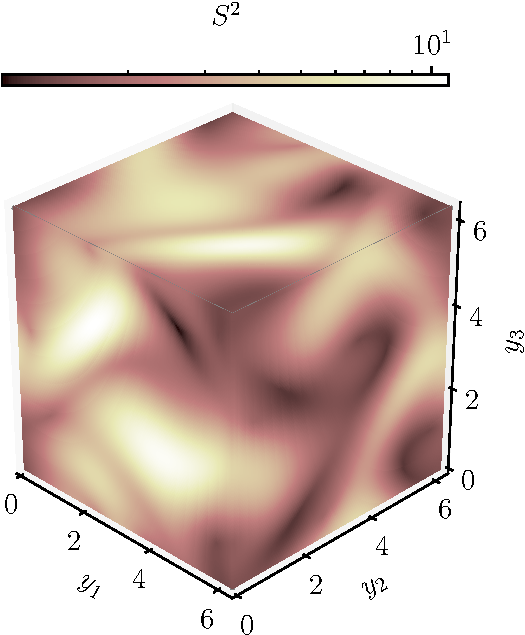
\includegraphics[width=\textwidth]{chp04_paper_numerics/figures/gabc/S2_box_1.0_cropped}
		% 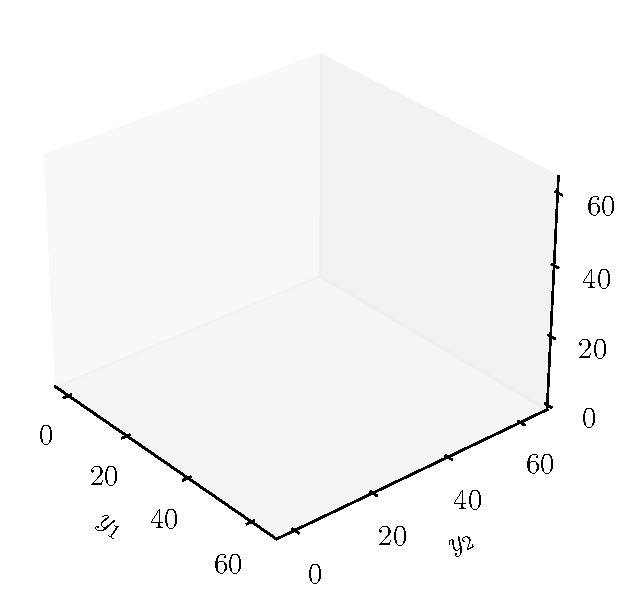
\includegraphics[width=0.49\textwidth]{chp04_paper_numerics/figures/gabc/robust_box_1}
		\caption{\(t = 1\)}
		\label{fig:gabc_S2_1}
	\end{subfigure}
	\begin{subfigure}[t]{0.49\textwidth}
		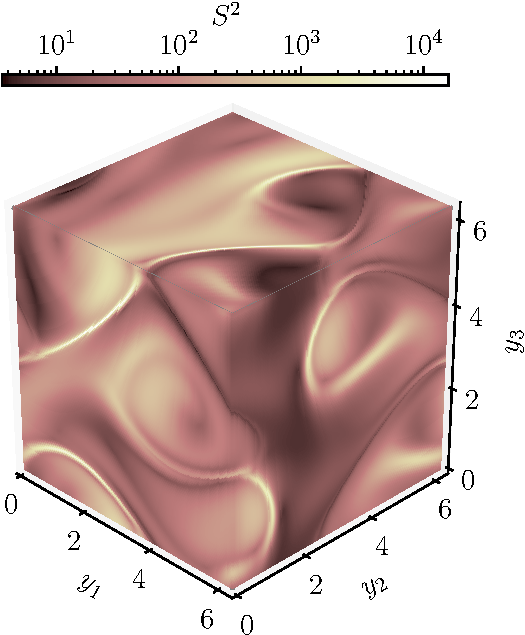
\includegraphics[width=\textwidth]{chp04_paper_numerics/figures/gabc/S2_box_3.0_cropped}
		% 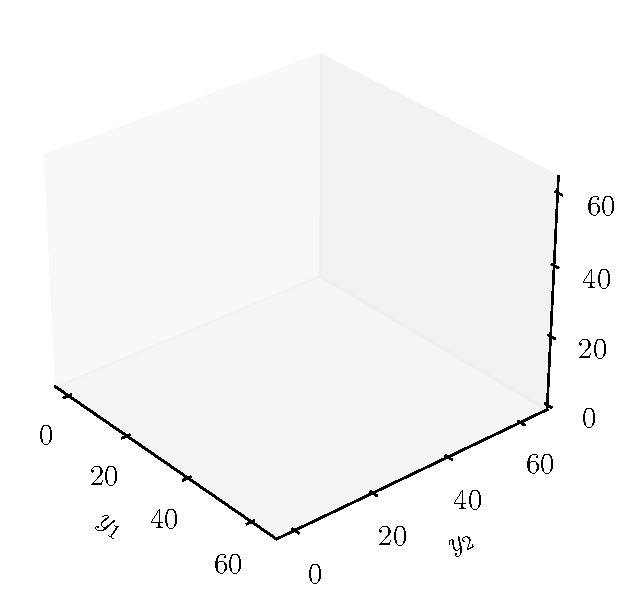
\includegraphics[width=0.49\textwidth]{chp04_paper_numerics/figures/gabc/robust_box_1}
		\caption{\(t = 3\)}
		\label{fig:gabc_S2_3}
	\end{subfigure}
	\caption{The stochastic sensitivity field for the GABC flow \cref{eqn:gabc} with identity diffusion, over the time interval \([0,t]\).}%, and robust sets (right) extracted with a threshold of \(R = 0.8\).}
	\label{fig:gabc_S2}
\end{figure}

To introduce 3-dimensional noise to the system, we set \(\sigma \equiv I\), the \(3 \times 3\) identity matrix, and compute stochastic sensitivity for a \(200\times 200\) grid of initial conditions on each face of the cube \([0,2\pi] \times [0,2\pi] \times [0,2\pi]\).
The spatial periodicity and symmetry of the dynamics means that these three faces are sufficient to describe the entire structure of the field within the region \citep{DombreEtAl_1986_ChaoticStreamlinesABC}.
As with the two-dimensional example, for each initial condition we compute the \(3 \times 3\) covariance matrix using the Mazzoni method.
The stochastic sensitivity value is then computed by taking the operator norm of this covariance matrix.
\Cref{fig:gabc_S2} plots the stochastic sensitivity on the three faces of the cube, at two different times.
At \(t = 1\) (\Cref{fig:gabc_S2_1}), the vortex structures are highlighted by the stochastic sensitivity field, in that these regions have a higher uncertainty due to the ??
\td{Interpret - looks like the vortex structures are hilighted by the field?}
When \(t = 3\) (\Cref{fig:gabc_S2_3}), the flow is domainated by chaotic mixing, but we nonetheless see structures highlighted by the stochastic sensitivity...!!!
In fact, these narrow ridge-like structures correspond to the unstable manifolds within the flow \citep{DombreEtAl_1986_ChaoticStreamlinesABC}: the repelling nature of these regions results in a `larger' stochasticity.

\section{Numerical validation and applications}\label{sec:numerics}

This section will validate the theory presented in \Cref{sec:theory}.
Following the example in Chapter 5 of \cite{SamelsonWiggins_2006_LagrangianTransportGeophysical}, we consider an unsteady meandering jet in two dimensions, which may serve as an idealised model of geophysical Rossby waves.
The velocity field for \(y \equiv \left(y_1, y_2\right)\) is given by \cite{SamelsonWiggins_2006_LagrangianTransportGeophysical}
\begin{equation}
	u\left(y, t\right) = \begin{bmatrix}
		c - A\sin\left(Ky_1\right)\cos\left(y_2\right) + \oldepsilon_{\mathrm{mj}} l_1\sin\left(k_1\left(y_1 - c_1 t\right)\right)\cos\left(l_1 y_2\right) \\
		AK\cos\left(Ky_1\right)\sin\left(y_2\right) + \oldepsilon_{\mathrm{mj}} k_1\cos\left(k_1\left(y_1 - c_1t\right)\right)\sin\left(l_1 y_2\right)
	\end{bmatrix}.
 \label{eqn:jet_ex}
\end{equation}
The velocity field describes a kinematic travelling wave with deterministic oscillatory perturbations in a co-moving frame.
Here, \(A\) is the amplitude and \(c\) is the phase speed of the primary wave, and \(K\) is the wavenumber in the \(y_1\)-direction.
The oscillatory perturbation has amplitude \(\oldepsilon_{\mathrm{mj}}\), phase speed \(c_1\) (in the co-moving frame), and wavenumbers \(k_1\) and \(l_1\) in the \(y_1\)- and \(y_2\)-directions respectively.
Throughout, we take the parameter values \(c = 0.5\), \(A = 1\), \(K = 4\), \(l_1 = 2\), \(k_1 = 1\), \(c_1 = \pi\), and \(\oldepsilon_{\mathrm{mj}} = 0.3\).
For these values, the flow consists of a meandering jet with vortex structures within the meanders, and a chaotic zone
which influences the fluid transfer between the jet and the vortices. 
All necessary flow map data is obtained by directly solving \eqref{eqn:ode_det} numerically, with the standard Euler scheme.
The flow map gradients required for computing the covariance matrix with \eqref{eqn:sigma_calc} are calculated via a star-grid finite-difference approximation, using a spatial resolution of \(0.001\). 

All simulations in this section were generated using the Julia programming language \cite{BezansonEtAl_2017_JuliaFreshApproach}, with implementations of the ordinary and stochastic differential equation solvers provided by the DifferentialEquations.jl package \cite{RackauckasNie_2017_DifferentialEquationsJlPerformant}.
All figures were created using the Makie.jl package \cite{DanischKrumbiegel_2021_MakieJlFlexible}.
The code is available as  \href{https://github.com/liamblake/explicit-gaussian-characterisation-uncertainty}{open source}\footnote{at \url{https://github.com/liamblake/explicit-gaussian-characterisation-uncertainty}.}.
%\sab{I don't think you need to put these codes in the supplementary materials if they are available open-source.}


\subsection{Validation of \Cref{thm:main}}
This section will validate the bound in \Cref{thm:main} directly, and illustrate the convergence of the SDE solution towards the expected Gaussian distribution described in \Cref{thm:gauss_dist}.
For each value of \(\epsilon\) considered, we use the Euler-Maruyama method \cite{KloedenPlaten_1992_NumericalSolutionStochastic} to generate \(N = 10000\) independent realisations of the solutions to \eqref{eqn:sde_y} and \eqref{eqn:limit_sde}.
A step size of \(\delta t = 10^{-4}\) is used to ensure that numerical error does not dominate over the theoretical predictions.
These solution samples are generated with the \emph{same} realisations of the Wiener process increments \(W_{t + \delta t} - W_t \sim \mathcal{N}\left(0, \delta t I_n\right)\).
We consider the initial condition \(x = \left(0, 1\right)\) and the prediction of the model at time \(t = 1\).
For each realisation of \(y_t^{(\epsilon)}\), a corresponding realisation of the scaled deviation \(z_t^{(\epsilon)}(x)\) is computed.
In the following, let \(\hat{z}_1^{(\epsilon)},\hdots, \hat{z}_N^{(\epsilon)}\) and \(\hat{z}_1,\hdots, \hat{z}_N\) denote the \(N\) realisations of \(z_t^{\left(\epsilon\right)}(x)\) and \(z_t(x)\) respectively.

\Cref{fig:y_hists} shows the resulting simulations of \(y_t^{(\epsilon)}\) for four different values of \(\epsilon\).
The realisations are binned as a histogram and bin counts are normalised, to provide an empirical estimate of the probability density function of \(y_t^{(\epsilon)}\).
Superimposed (in solid black) are the first, second and third standard-deviation contours of the probability density function of the Gaussian approximation \eqref{eqn:y_t_gauss}.
The first three standard-deviation levels of the \(2\times 2\) sample covariance matrix of the realisations, are also overlaid (in dashed blue).
% If the observations were distributed according to a bivariate Gaussian distribution with that corresponding covariance matrix, then approximately \(86.47\%\) of the data lies within the first two bounds, and \(98.89\%\) within all three \cite{WangEtAl_2015_ConfidenceAnalysisStandard}.
As \(\epsilon\) decreases towards \(0\), the samples increasingly resemble a Gaussian distribution, and both the mean and covariance coincide with the corresponding limits.

\begin{figure}[htbp]
	\begin{center}
        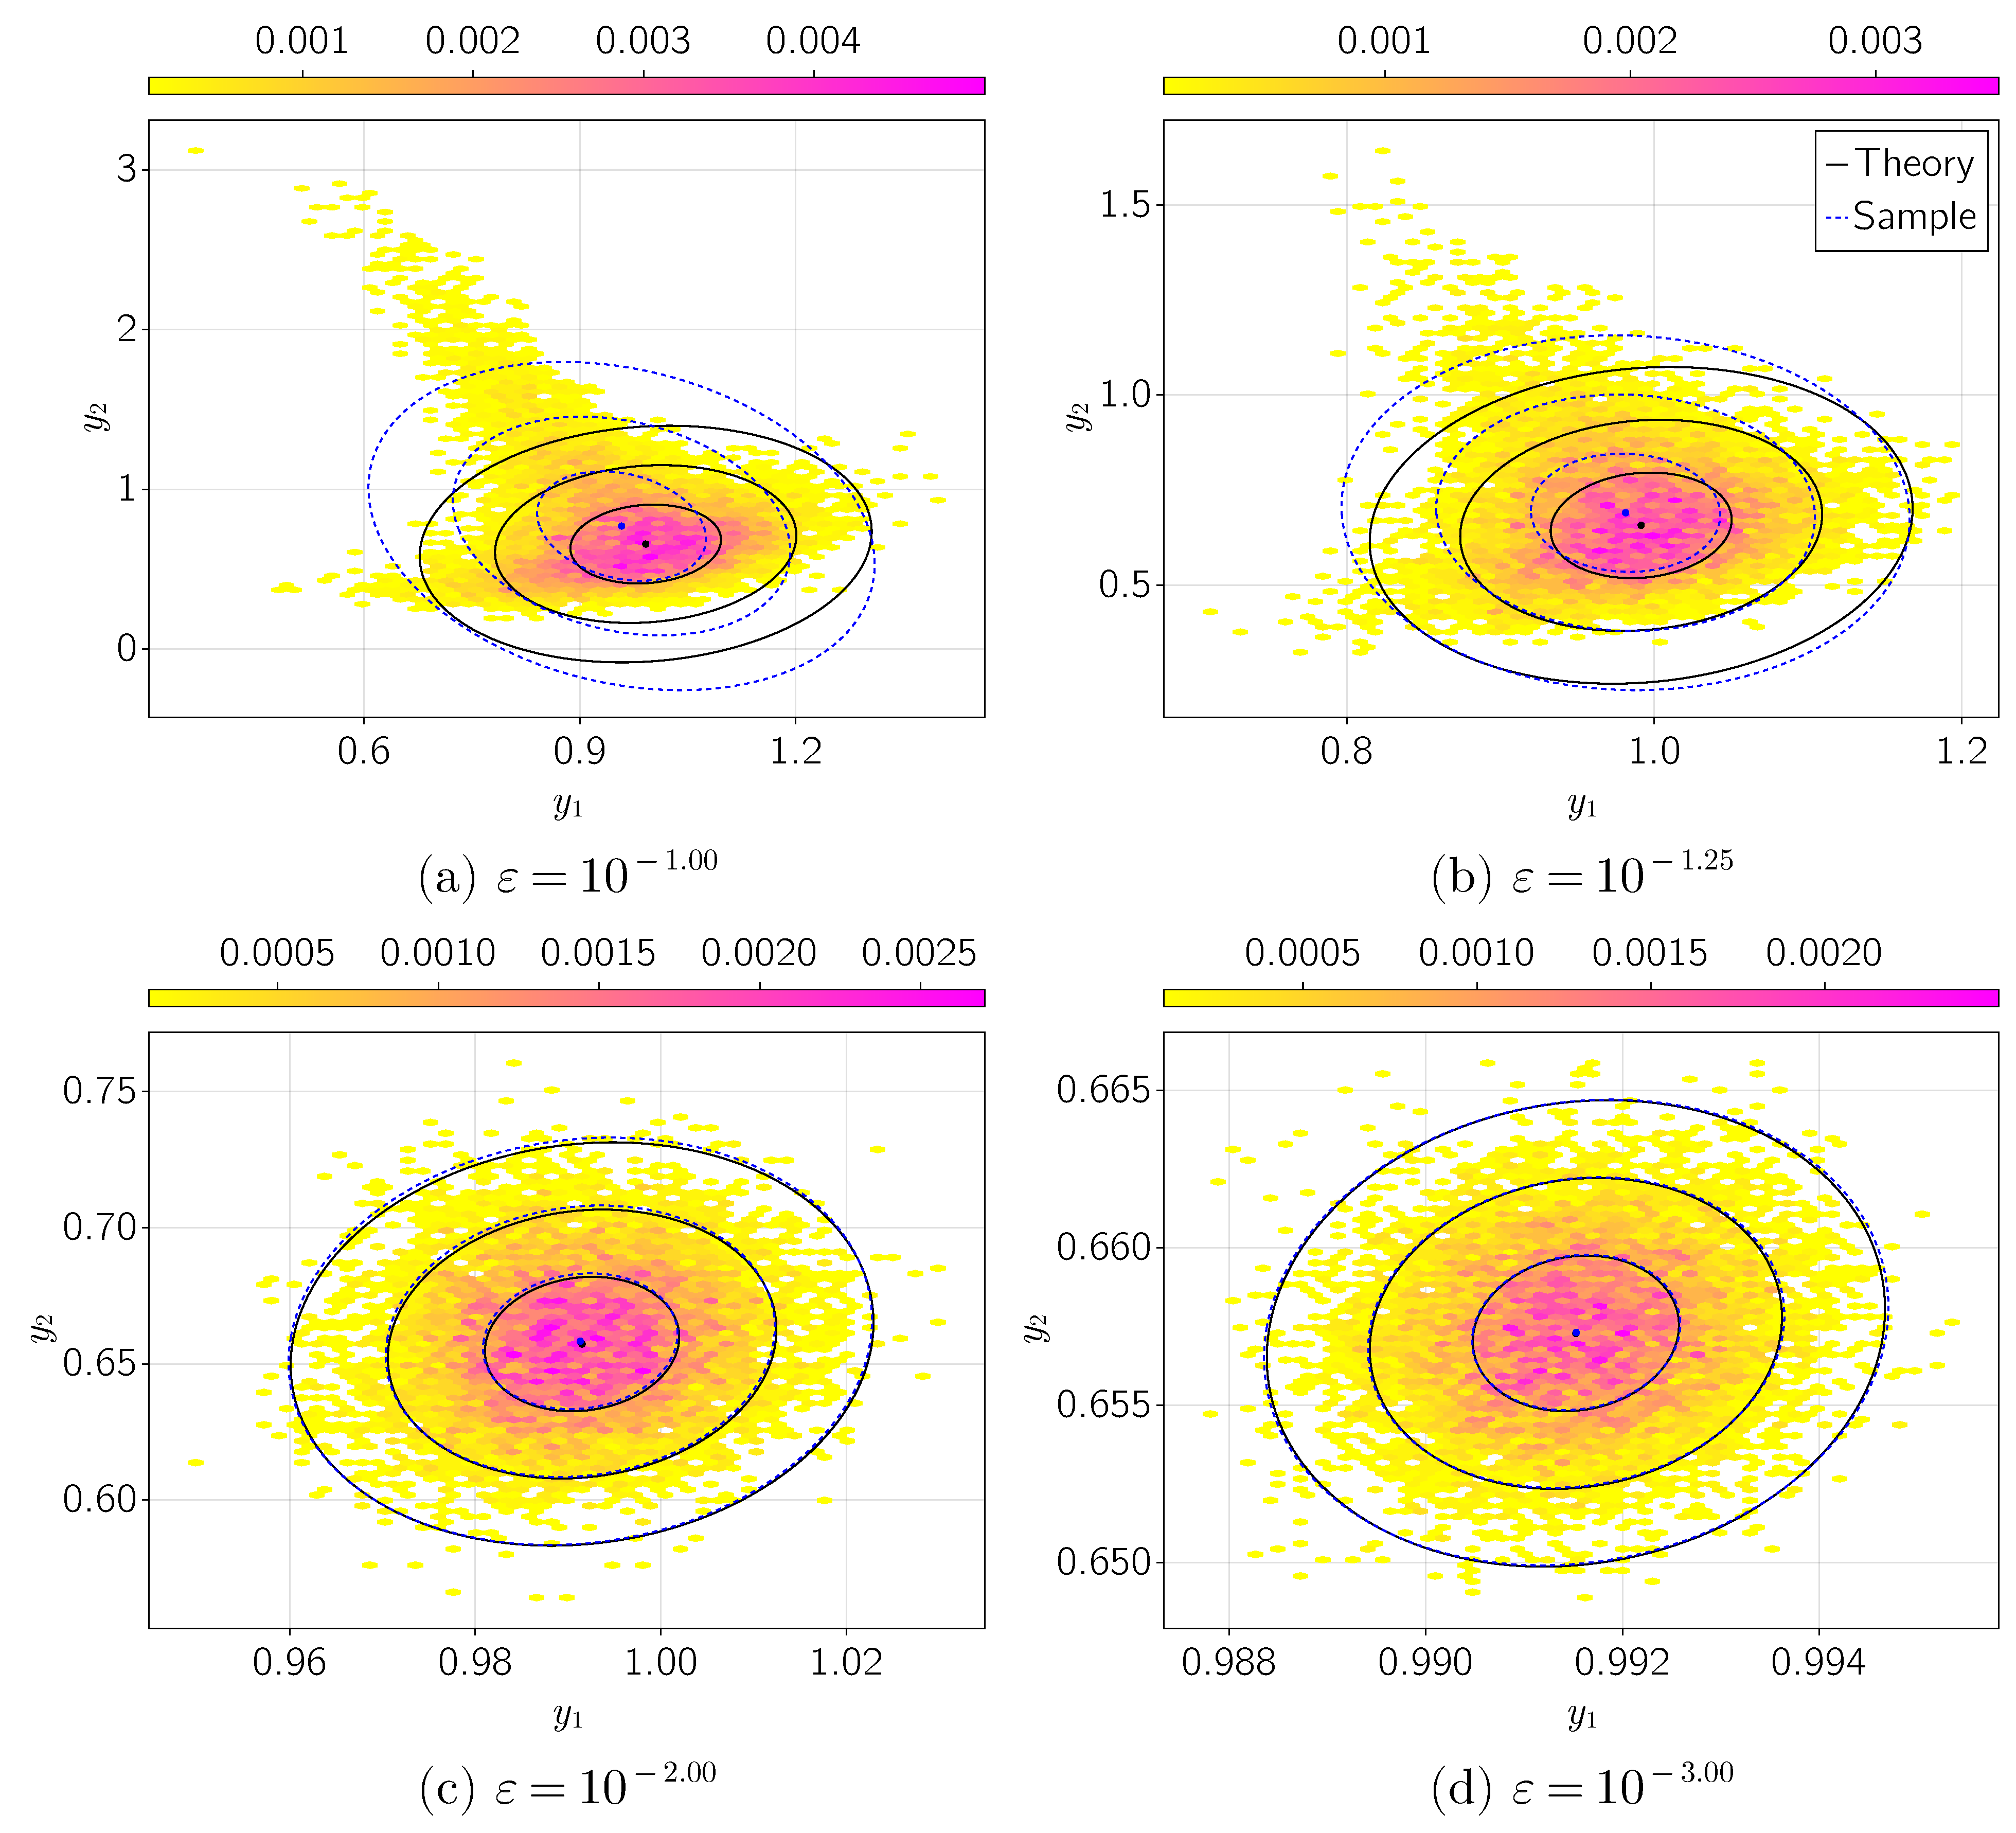
\includegraphics[width=\textwidth]{paper1_gaussian_limit/figures/y_histogram.pdf}       
				% \td{Increase size/clarity of points at centre of contours}
		\caption{Histograms of \(y_t^{(\epsilon)}\) from direct simulation of \eqref{eqn:sde_y}, for four different \(\epsilon\) values.
		Overlaid in black are contours of the Gaussian limit \eqref{eqn:y_t_gauss}, which correspond to the first three standard deviation levels centred at the limiting mean \(F_0^t(x)\).
        In dashed blue are corresponding contours computed from the sample covariance matrix of the realisations.
        }
		\label{fig:y_hists}
	\end{center}
\end{figure}

To directly validate \Cref{thm:main} for \(r \geq 1\), define the error metric
\[
	\Gamma_z^{\left(r\right)}\!\left(\epsilon\right) \coloneqq \frac{1}{N}\sum_{i = 1}^{N}{\norm{\hat{z}_{i}^{(\epsilon)} - \hat{z}_i}^r},
\]
which is an estimator of the right-hand side of \eqref{eqn:main_ineq}.
For \(r = 1,2,3,4\), \(\Gamma_z^{\left(r\right)}\!\left(\epsilon\right)\) is shown (in a logarithmic scale) for decreasing values of \(\epsilon\) in \Cref{fig:gamma_z_valid}.
\Cref{thm:main} predicts that \(\log_{10}\left(\Gamma_z^{\left(r\right)}\left(\epsilon\right)\right)\) should decay linearly with a slope greater than \(r\) as \(\epsilon\) decreases to zero.
The lines of best fit for each value of \(r\) in \Cref{fig:gamma_z_valid} show this behaviour, and are therefore consistent with \Cref{thm:main}.

\begin{figure}[htbp]
	\begin{center}
        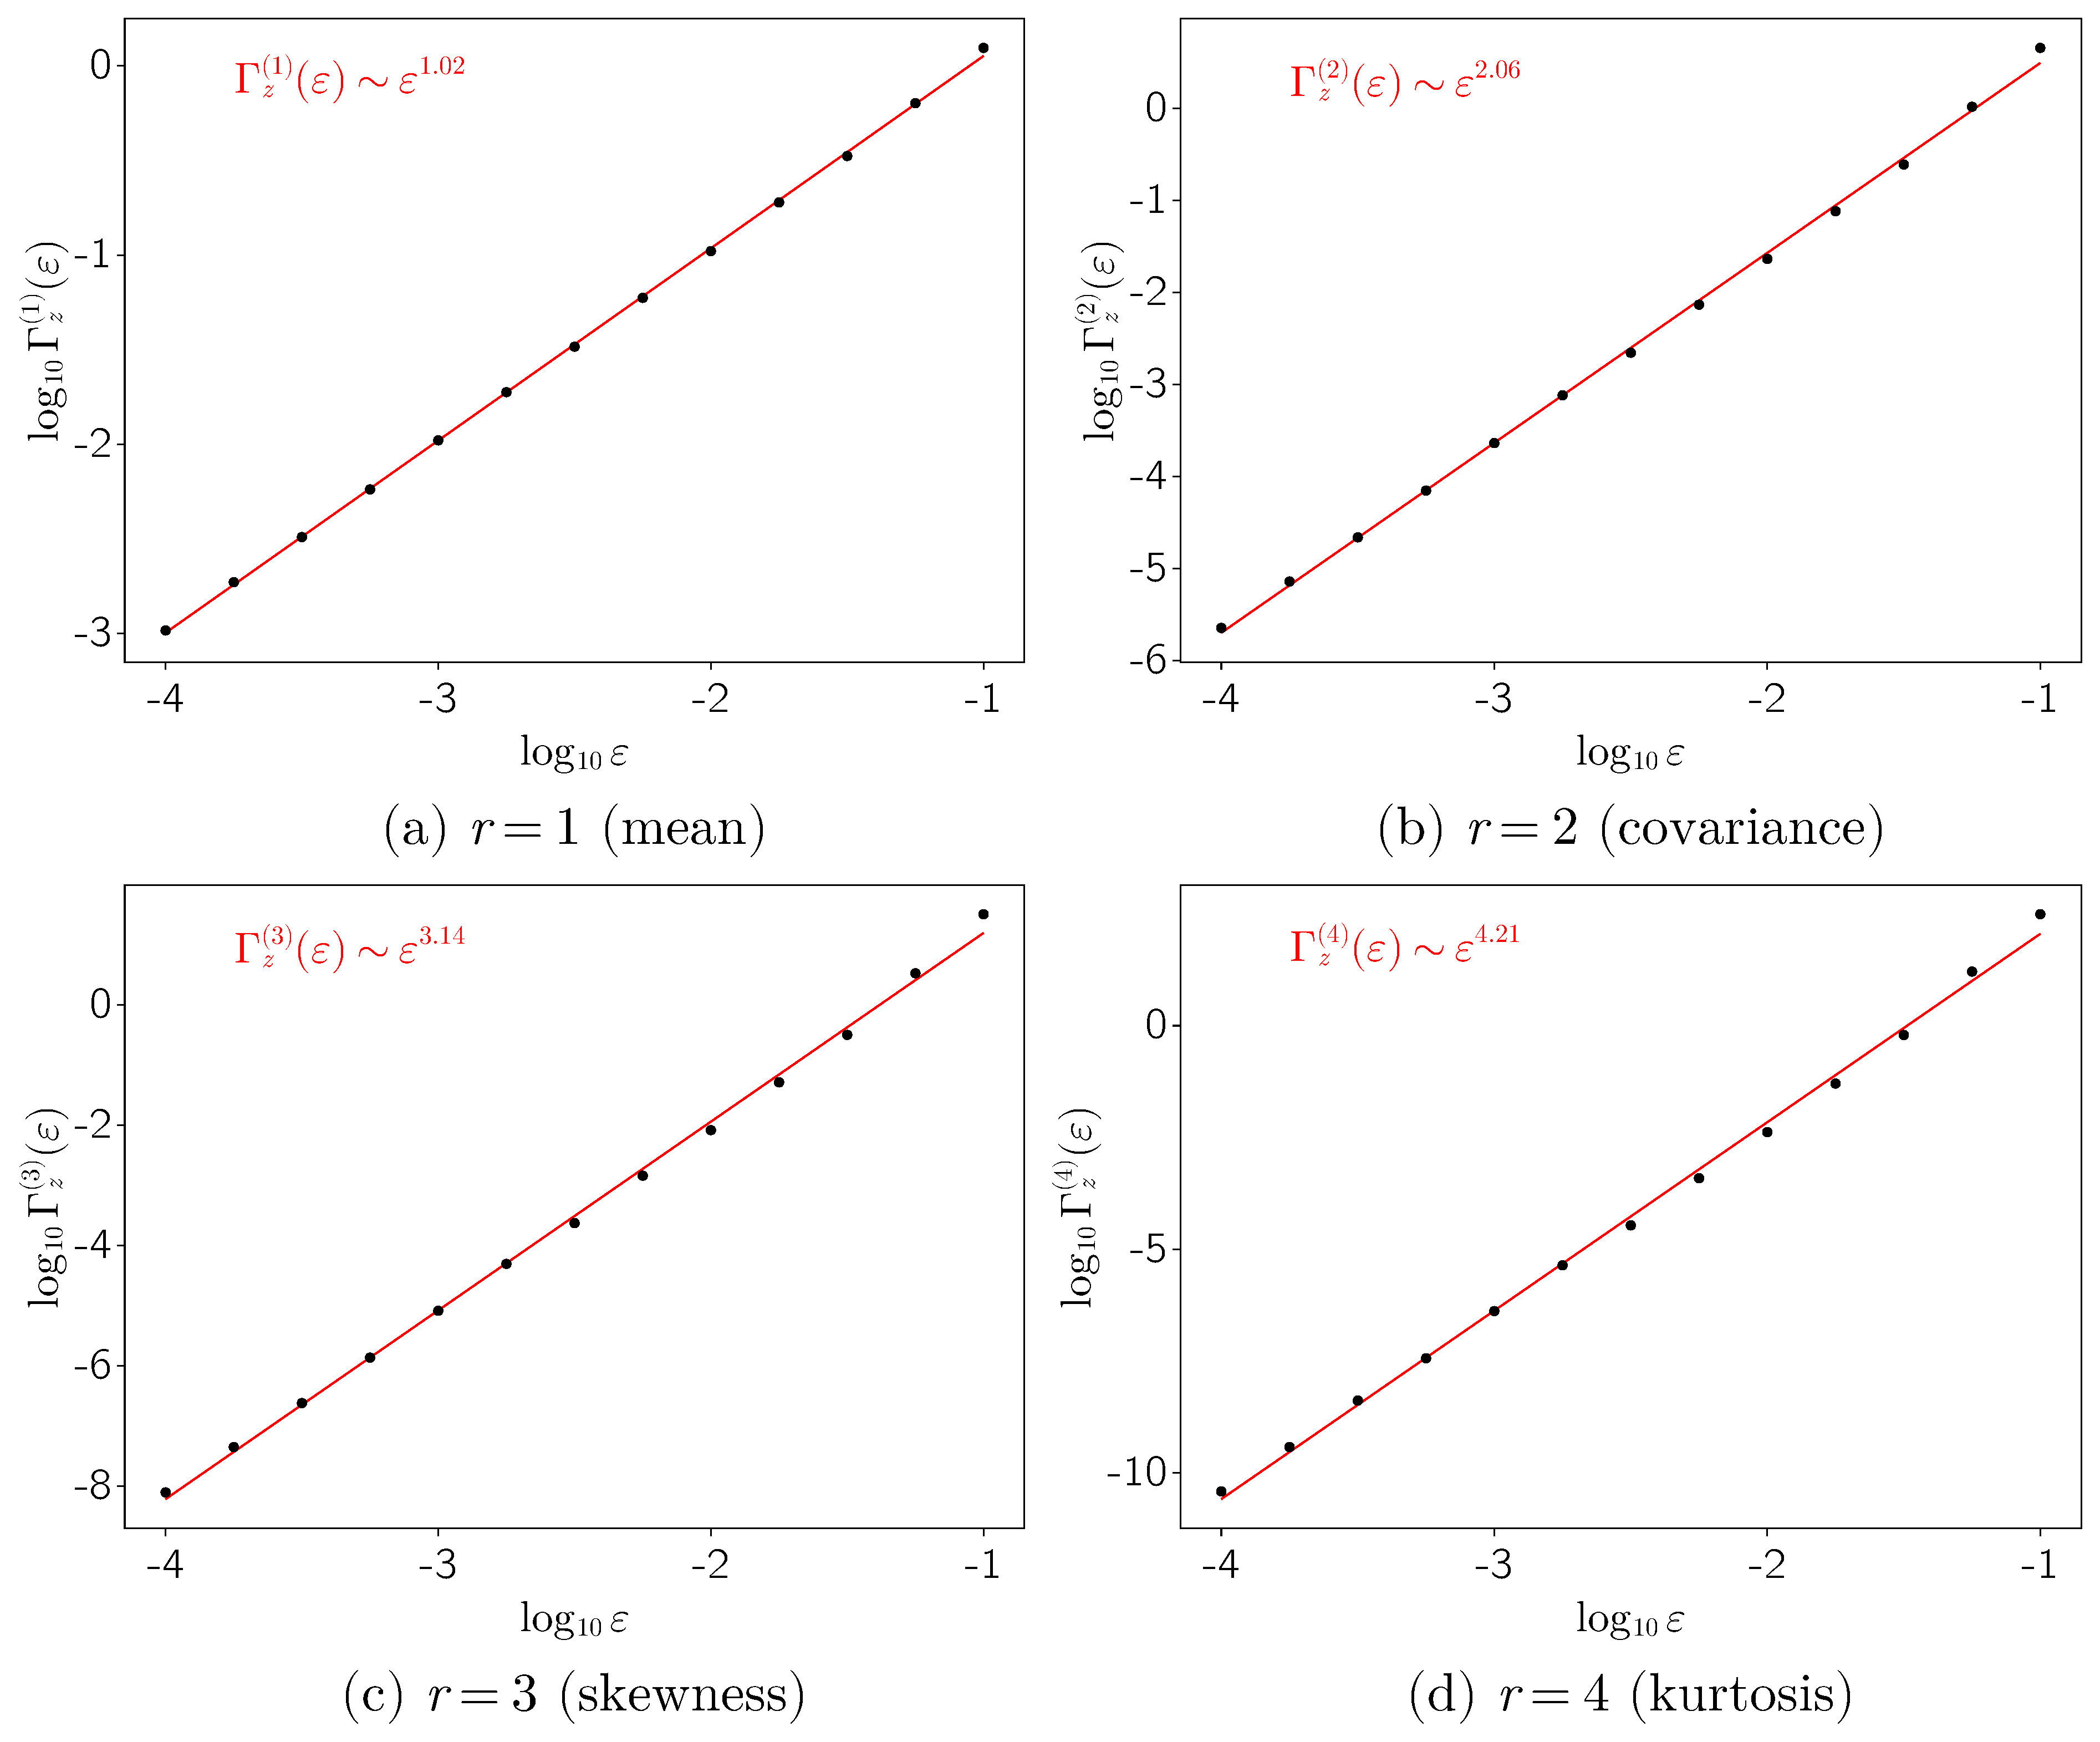
\includegraphics[width=\textwidth]{paper1_gaussian_limit/figures/z_diff.pdf}
		\caption{Validation of \Cref{thm:main}, by plotting the sample \(r\)th raw moment distance (the error metric \(\Gamma_z^{(r)}(\epsilon)\)) between \(10000\) realisations of \(z_t^{(\epsilon)}(x)\) and \(z_t(x)\), for decreasing values of \(\epsilon\).
        A line of best fit (in red) is placed on each, and the resulting slope indicated.}
		\label{fig:gamma_z_valid}
	\end{center}
\end{figure}


%%%%%%%%%%%%%%%%%%%%%%%%%%%%%%%%%%%%%

\subsection{The evolution of \(\Sigma(x,t)\) through time}
Here we shall illustrate that the limiting covariance matrix \(\Sigma\) captures the time-evolution of model uncertainty.
Consider the same meandering jet model in \eqref{eqn:jet_ex}, with the parameter values used in the previous subsection.
We fix the noise scale parameter at \(\epsilon = 0.03\) and consider the evolution of the stochastic solution to \eqref{eqn:sde_y} and the limiting Gaussian distribution \eqref{eqn:y_t_gauss} for times \(t\) in the interval \([0,1]\).
We also consider two different choices of the diffusion matrix \(\sigma\): the identity as before, and
\begin{align}
\label{eq:sigM}
\sigma_M(x) \coloneqq \begin{bmatrix}
       x_1 & 0.5 \\ 
       x_1 & 0.5\left(x_1 + x_2\right)
\end{bmatrix},
\end{align}
to include both multiplicative and non-diagonal noise which grow for larger values of the coordinates. 


\begin{figure}[htbp]
	\begin{center}
        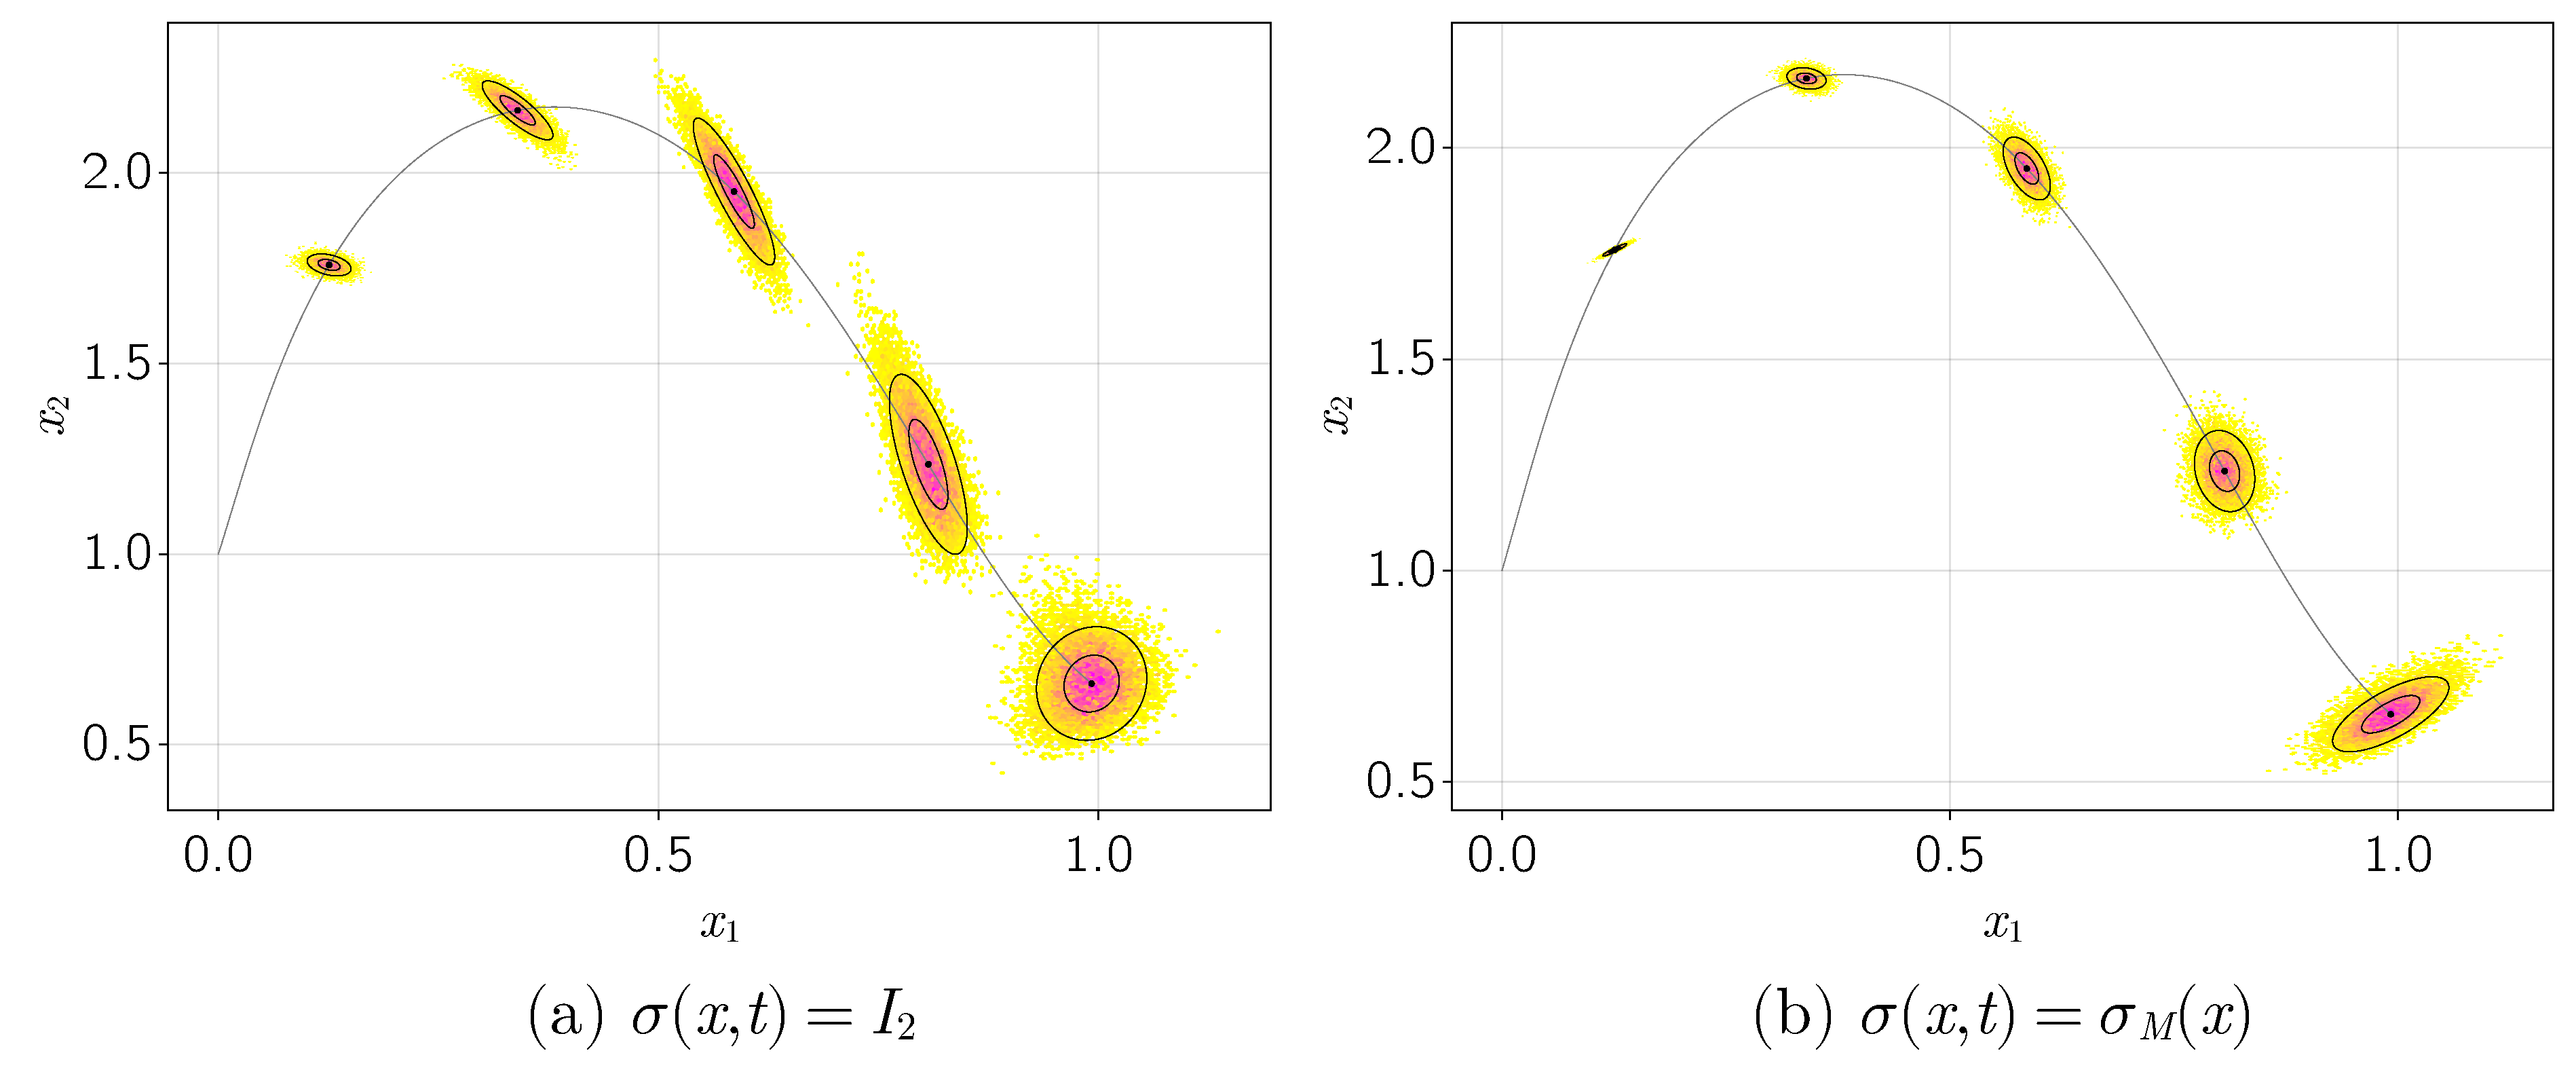
\includegraphics[width=\textwidth]{paper1_gaussian_limit/figures/through_time.pdf}
				\caption{Histograms of \(y_t^{(0.03)}\) for (from left to right) \(t = 0.2, 0.4, 0.6, 0.8, 1.0\), with the time-evolution of the deterministic trajectory in grey and contours of the limiting covariance matrix \eqref{eqn:sigma_calc} for each time. The right figure uses the diffusion matrix $\sigma_M(x)$ as defined in \eqref{eq:sigM}.}
        % (c,d) The time-evolution of \(S^2(x,t)\) and the operator norm of the sample covariance for stochastic simulations of \(y_t^{(0.3)}\) at each time.}
        \label{fig:time_evol}
  \end{center}
\end{figure}

\Cref{fig:time_evol} plots histograms of realisations of the solution to \eqref{eqn:sde_y} at several different times, evolving from the same initial condition \(x = \left(0, 1\right)\), and the time-evolution of the corresponding deterministic trajectory solving \eqref{eqn:ode_det}. 
Overlaid on each histogram are the contours of the limiting Gaussian distributions, computed entirely from covariance matrix \eqref{eqn:sigma_calc}.
Although each distribution is non-Gaussian, the evolution of the uncertainty distribution through time is captured by \(\Sigma\).
For examples, features of the error distributions, such as stretching and rotation, are reflected in \(\Sigma\).
This remains the case even when the noise is multiplicative with \(\sigma = \sigma_M\).
The computation of \(\Sigma\) circumvents the need for expensive Monte-Carlo simulation to draw conclusions about such evolution of uncertainty.


% \note{Removing \(S^2\) here - doesn't add much and saves space.}
% To further illustrate that the time-evolution of uncertainty is captured by the limiting covariance, we also consider the stochastic sensitivity values.
% As highlighted in \Cref{sec:theory_s2}, the operator norm of a covariance matrix provides a scalar measure of uncertainty, independent of the fluid flow context.
% We compute the operator norm of the sample covariance matrix of the realisations, to provide a scalar estimate of the true uncertainty, and plot this against time alongside the limiting \(S^2(x,t)\) values in \Cref{fig:time_evol}(c,d).
% The \(S^2(x,t)\) closely matches the corresponding sample values.

% The limiting covariance matrix \(\Sigma\) and the \(S^2\) measure can therefore capture the time-evolution of model uncertainty, even though these uncertainty distributions are non-Gaussian, without resorting to stochastic simulation.
% Even when the noise is multiplicative and non-diagonal, features such as stretching of the error distribution, and the direction of most uncertainty, are reflected in \(\Sigma\).

%%%%%%%%%%%%%%%%%%%%%%%%%%%%%%%%%%%%%

% \subsection{Stochastic sensitivity as a coherence measure}
% We will now demonstrate the computability of the stochastic sensitivity measures,
% not in detail as a tool for coherent structure extraction (other examples in 2D are provided by \cite{BadzaEtAl_2023_HowSensitiveAre,Balasuriya_2020_StochasticSensitivityComputable}) but to instead illustrate the operator norm computation in \eqref{eqn:s2_calculation}.
% %\sab{While you say that you want to establish consistency, how do you do it?  It's not clear you've computed it using the filthy formulas from the original, for comparison.  Perhaps it's better to just say that you've compared them (after all, the expressions are identical), and that this section demonstrates computability of this coherence measure?}

% \begin{figure}
% 	\begin{center}
% 		\includegraphics[width=\textwidth]{figures/s2_field_0.3.pdf}
% 		\caption{(Left) The logarithm of the \(S^2\) field, for the meandering jet flow over the time interval \([0,1]\), computed directly from the limiting covariance matrix \(\Sigma\left(x,1\right)\).
%  			The natural logarithm is taken to improve visibility of structures within the fields.
%  			(Right) Robust sets (in blue) extracted from the stochastic sensitivity field using a threshold value of 10.}
% 		\label{fig:s2_field}
% 	\end{center}
% \end{figure}

% We again consider the meandering jet \eqref{eqn:jet_ex} take \(\sigma \equiv I\) and consider initial conditions in the spatial domain \(\Omega_0 \coloneqq \left[0, \pi\right] \times \left[0, \pi\right]\).
% A grid of \(800 \times 800\) initial conditions is uniformly seeded in \(\Omega_0\).
% For each initial condition \(x\), the covariance matrix \(\Sigma(x,1)\) is computed with \eqref{eqn:sigma_calc}, and the corresponding \(S^2\) value is calculated by taking the operator norm.
% \Cref{fig:s2_field} shows the logarithm of the \(S^2\) field on \(\Omega_0\) from time \(0\) to \(t = 1\), 
% In a bid to extract ``coherent'' regions, we extract subsets of \(\Omega_0\) using the \(S^2\) field, by taking a threshold of $ 10 $.
% The \(S^2\) field is largest in the elongated gyre regions outside of the meandering jet, where the flow exhibits chaotic behaviour \cite{Pierrehumbert_1991_ChaoticMixingTracer} and we accordingly expect larger uncertainty due to the model dynamics.
% As a region of small \(S^2\) value, the meandering jet emerges as a coherent structure, consisting of initial points whose eventual fate is significantly more certain than in other regions. 


%%%%%%%%%%%%%%%%%%%%%%%%%%%%%%%%%%%%%%%%%%%%%%%%%%%%%%%%%%%
% \input{discussion}
\section{Discussion}\label{sec:paper1_appl}

This paper has contributed a rigorous justification, in terms of error bounds and a small-noise limit, for an easily computable linearisation approximation to the solution of nonlinear stochastic differential equations, as seen across diverse places in the literature \cite[e.g.]{Jazwinski_2014_StochasticProcessesFiltering, Sanz-AlonsoStuart_2017_GaussianApproximationsSmall, SarkkaSolin_2019_AppliedStochasticDifferential}.
The theory applies to fully non-autonomous SDEs with multiplicative noise. 
This result extends the convergence bound on the Kullback-Leibler divergence by Sanz-Alonso and Stuart \cite{Sanz-AlonsoStuart_2017_GaussianApproximationsSmall} to an explicit bound on the convergence of all moments of the difference between the exact SDE solution and the approximation, and further establishes the exact Gaussian distribution in the small-noise limit. While it is known that convergence of the KL divergence leads to convergence of the moments \cite{LuEtAl_2017_GaussianApproximationsProbability}, this manuscript provides the exact rate of that convergence.
Our bound is verified numerically by plotting the first four raw moments of the distance between the true noise-scaled solution and the linearised solution (see \Cref{fig:gamma_z_valid}). 
The results, plotted across three orders of magnitude of the small noise parameter, match our theoretical prediction exactly. 

In addition, we described a framework in which uncertainty in deterministic models can be ascribed without the need for expensive stochastic simulation, and purely from the deterministic solution dynamics.
We illustrated how the Gaussian limit reflects the time-evolution of uncertainty (see \Cref{fig:time_evol}), even when the true uncertainty distributions are themselves non-Gaussian.

A powerful advantage of this framework is that the diffusivity matrix \(\sigma\) is permitted to vary spatio-temporally, allowing for multiplicative noise.
Multiplicative noise is often ignored in practice, due to difficulties in working with analytically (see, for instance, the prior lack of rigourous justification of linearisations when the noise is multiplicative) and generating numerical realisations efficiently (e.g. the review in \cite{MoraEtAl_2017_StableNumericalScheme}).
It has also been shown that multiplicative noise on linear dynamics can model departures from Gaussianity observed in climate statistics \cite{SuraEtAl_2005_MultiplicativeNoiseNonGaussianity}, as opposed to nonlinear dynamics with only additive noise. 
The spatio-temporal dependence of \(\sigma\) can also capture experimental and observational considerations that are otherwise ignored in the deterministic model, such as cloud cover when using satellite measurements or nonuniform uncertain across the field of view of a camera.
% The multiplicative noise is captured by the Gaussian approximation by evaluating \(\sigma\) along the deterministic reference trajectory.
% The Gaussian uncertainties capture both the model dynamics, and any multiplicative or spatiotemporal dependence in the uncertainty, through specification of \(\sigma\).
We therefore present a highly flexible framework that can capture any prior knowledge of non-uniform uncertainty that arises from modelling or experimental considerations.

This paper also supplied theoretical and computational extension to the ``stochastic sensitivity'' tools introduced by Balasuriya \cite{Balasuriya_2020_StochasticSensitivityComputable}.
Stochastic sensitivity was hitherto derived as the variance of an unknown limiting distribution and could only be computed in two spatial dimensions: we established that stochastic sensitivity, in any number of dimensions, is computable as the operator norm of the covariance matrix of our limiting SDE. 
We have also established that the limiting distribution in question is Gaussian, which may provide insight into properties of stochastic sensitivity as a means of uncertainty quantification in any model (not just in the fluids context) where an $ n $-dimensional state variable evolves according to a ``best available" model.

The Gaussian approximation presented here arises as the leading order term in a power series expansion of the SDE solution in terms of the noise scale parameter \(\epsilon\) \cite{Blagoveshchenskii_1962_DiffusionProcessesDepending}.
A further extension would be to explore the higher-order terms in such an expansion, which could lead to a practical framework for constructing higher-order characterisations and approximations of the stochastic solution.
However, the higher-order terms are known to be individually non-Markovian, and satisfy non-linear SDEs for which the solution is not expected to be analytically available \cite{Blagoveshchenskii_1962_DiffusionProcessesDepending}.

In this paper, we have assumed throughout that the initial condition \(x\), from which both the stochastic differential equation and the deterministic flow map evolves from, is \emph{certain} (i.e. not a random quantity).
However, in practice there is uncertainty associated with the initial state which should also be accounted for.
The bound in \Cref{thm:main} is independent of the initial condition, suggesting that the required extension of the theoretical result is straightforward.
This extension will broaden our framework, allowing for uncertainties in \emph{both} the initial state and the time-evolution of the model to be characterised at once in a precise sense.

Similarly, we assume that the reference deterministic model \eqref{eqn:ode_det} for the evolution of the state variable is ``correct'' and known exactly, in that in the absence of any noise (i.e. \(\varepsilon = 0\)), the SDE model \eqref{eqn:sde_y} reduces to the deterministic \eqref{eqn:ode_det}. 
The Gaussian characterisation is computed from knowledge of either the driving vector field or the solution data itself, i.e. the flow map.
However, these components of the deterministic model may not be known exactly, e.g. from solving \eqref{eqn:ode_det} numerically, interpolation error, etc.
There is a need to extend the theory presented here to account for this case; to, for instance, establish a bound in the error between the SDE solution and the limiting Gaussian, as in \Cref{thm:main}, if the Gaussian distribution is constructed from an ``incorrect'' deterministic model.
Both of these theoretical extensions, to uncertain initial conditions and incorrect deterministic dynamics, are currently being pursued.


\subsection{Applications}

Here, we briefly discuss some anticipated applications of this work across a wide range of fields, including climate and ocean modelling, data assimilation and Lagrangian coherent structures.

This work fits in with recent interest in stochastic parameterisation as a means to account for unresolved subgrid effects in climate modelling \cite{BernerEtAl_2017_StochasticParameterizationNew,LeutbecherEtAl_2017_StochasticRepresentationsModel,Palmer_2019_StochasticWeatherClimate}. 
In particular, the recent review \cite{LeutbecherEtAl_2017_StochasticRepresentationsModel} concludes, ``The aim of current and future developments in stochastic representations of model uncertainty is to develop schemes that are computationally highly efficient and contribute only moderately to the overall computational cost...''.
This paper provides one method to convert a stochastic parameterisation (formulated as a SDE) to a computationally cheaper set of coupled ODEs for the mean and variance of an approximate Gaussian, together with a convergence proof and error estimates. 

To ascribe uncertainties directly onto the deterministic model, we assume that the diffusivity matrix \(\sigma\) is specified \textit{a priori}, to capture any known multiplicative noise effects.
There are methods for estimating \(\sigma\) directly from observed data, e.g. the Bayesian inference approach of \cite{YingEtAl_2019_BayesianInferenceOcean} or via statistical estimation as in \cite{CotterPavliotis_2009_EstimatingEddyDiffusivities}, which can be used in our framework.
In particular, \cite{YingEtAl_2019_BayesianInferenceOcean} relies upon computationally expensive numerical approximations to compute the likelihood of each trajectory, whereas from this paper we have a potentially more efficient computation, using the analytically available Gaussian limit.
Coupling these approaches with the approximation here could provide a complete and practical framework to characterise the uncertainty in the flow by efficiently estimating the (multiplicative) diffusion from observed trajectory data.

Data assimilation is a framework for improving uncertainties in predictions by combining model forecasts with observational data, accounting for error in both, and uncertainty quantification refers to the broader goal of capturing the uncertainty inherent in prediction \cite{BudhirajaEtAl_2019_AssimilatingDataModels,Jazwinski_2014_StochasticProcessesFiltering,LawEtAl_2015_DataAssimilationMathematical,ReichCotter_2015_ProbabilisticForecastingBayesian}.
The Gaussian limit here provides a characterisation of model uncertainty, and may therefore be useful in data assimilation and uncertainty quantification.
The linearisation of the stochastic differential equation \eqref{eqn:sde_y} used to construct the Gaussian approximation has been employed in data assimilation, e.g. in the continuous time continuous state-space extended Kalman filter \cite[\S 9]{Jazwinski_2014_StochasticProcessesFiltering}. The convergence analysis of this paper could contribute a new term, estimating the error due to linearisation, to the \emph{forecast uncertainty} covariance matrix employed in these extended Kalman filters. 

% There are several methods for computing the flow map gradient directly from observed tracer data, in the context of calculating finite-time Lyapunov exponents (FTLEs) \cite{Leung_2013_BackwardPhaseFlow, RabenEtAl_2013_ComputationFinitetimeLyapunov}.
% Another question would be whether the techniques of estimating the flow map gradient in the LCS literature can be coupled with a data assimilation scheme, by using the characterisation of the Gaussian approximation in terms of solely the flow map gradients.


% Speaking more generally, determining the structure of the model error 
% More complications arise if this model error is state (e.g. position) dependent, which is expected in many contexts \cite{Bishop_2019_DataAssimilationStrategies}.
% The work here presents a framework for computing a state-dependent model error covariance matrix entirely from the deterministic model dynamics.
% \td{Are we implicitly extending EKF to state-dependent covariances?}

% As an alternative, there are recent DA approaches that directly use coherent structures \cite{MacleanEtAl_2017_CoherentStructureApproach, Schlueter-KuckDabiri_2019_ModelParameterEstimation}, for which stochastic sensitivity could be applied to use coherent structures that reflect model certainty.

Stochastic sensitivity provides a novel method for extracting Lagrangian coherent structures (LCSs) \cite{BalasuriyaEtAl_2018_GeneralizedLagrangianCoherent, HadjighasemEtAl_2017_CriticalComparisonLagrangian} from fluid flow, by considering regions with uncertainty (as measured by the stochastic sensitivity field) below a prescribed threshold. 
Whereas the original formulation in \cite{Balasuriya_2020_StochasticSensitivityComputable} was restricted to two-dimensional flows, here we have an extension of the LCS extraction scheme to arbitrary dimensions. 

% LCS extraction has recently been used as a means of dimension reduction in data assimilation schemes \cite{MacleanEtAl_2017_CoherentStructureApproach,MorzfeldEtAl_2018_FeaturebasedDataAssimilation,Schlueter-KuckDabiri_2019_ModelParameterEstimation}.
% Through stochastic sensitivity, we have a method for extracting coherent regions that directly reflect model uncertainty, and so may be applicable in these DA schemes.

Moreover, most traditional LCS measures are completely deterministic measures, not accounting for any uncertainty in the driving velocity field, and the sensitivity of these methods to such uncertainty has not been investigated in detail. 
The robustness of several LCS methods to stochastic noise has recently been explored in \cite{BadzaEtAl_2023_HowSensitiveAre}, but via stochastic simulation and summary statistics. 
In this paper we have presented a theoretical result for characterising Lagrangian trajectory uncertainty, which can be used to perform a purely theoretical analysis of such sensitivity in LCS computations.
An initial study into the impact of uncertainty of one such method -- the finite-time Lyapunov exponent -- has already been performed using stochastic sensitivity \cite{Balasuriya_2020_UncertaintyFinitetimeLyapunov}, albeit in only two-dimensions and without knowledge that the limiting distribution is Gaussian.

